\documentclass[
fontsize=10pt,
font-family=lmodern,
languages={american,french}, % 'british' ou 'american' (pas 'english' !)
main-language=american,
load-style=dg,
title-font-family=sans-serif,
header-style=chapter-section,
bibliography-style=dg,
setspace=single
]{mines-albi-these}

\usepackage{pdflscape}
\usepackage[ruled,lined]{algorithm2e}

% les glossaires (index et nomenclature)
\makeglossaries
% ------------------------------------------------------------
% déclaration des acronymes (pour l'index)
% ------------------------------------------------------------

\newacronym{IMT}{IMT}{Institut Mines-Télécom : depuis 2017, intégration
  dans un seul institut des écoles de télécom et de la plupart des
  écoles des mines, sous la tutelle du ministère de l’Économie et des
  Finances.}

%%% Local Variables:
%%% mode: latex
%%% TeX-master: "../ma-these"
%%% End:

% ------------------------------------------------------------
% déclaration des symboles (pour la nomenclature)
% ------------------------------------------------------------

\newsymbolentry{sigma}{
  type=greek letter,
  sort={sigma},
  name={$\sigma$},
  description={Tension superficielle},
  unit={\si{\N\per\m}},
}

\newsymbolentry{Scap}{
  type=alphanumeric,
  sort={Scap},
  name={\ensuremath{S_{cap}}},
  description={Surface de la section du capillaire},
  unit={\si{\square\m}},
}

%%% Local Variables:
%%% mode: latex
%%% TeX-master: "../ma-these"
%%% End:


% pour la couverture
\usepackage{mines-albi-these-frontpage}

% une source de références bibliographiques
\addbibresource{bibliographie/ma-biblio.bib}

% la méta-information (dans le PDF et éventuellement sur la couverture)
\author{Julien Coche}
\title{Design of a social media processing system for crisis response: extraction, management, and delivery of relevant information for decision-makers.}
\date{14 février 2021} % date prévue de soutenance

\begin{document}

%----------------------------------------
\frontmatter


\makefrontpage{
  %% ----------------------------------------
  %% bandeau (à supprimer en version finale
  label=Not the final version of the document,
  %% ----------------------------------------
  %% thèse délivrée par
  granted by=imt mines albi,
  %% ----------------------------------------
  %% unité de recherche (utilisée les valeurs prédéfinies si possible)
  new research unit={mon labo}{LRSC -- Laboratoire de Recherche Super Chouette},
  research unit=mon labo,
  %% ----------------------------------------
  %% école doctorale (utilisée les valeurs prédéfinies si possible)
  new phd school={ednew}{EDNew : une nouvelle école doctorale},
  phd school=ednew,
  %% ----------------------------------------
  %% l'auteur (à décommenter si différent de la méta-information)
  % full name={Prénom Nom},
  %% ----------------------------------------
  %% la date de soutenance prévue (à décommenter si différent de la méta-information)
  % date={1\up{er} décembre 2099},
  %% ----------------------------------------
  %% le titre (à décommenter si différent de la méta-information)
  % title={Un titre très long qui donne envie de lire toute la thèse},
  %%  ----------------------------------------
  %% la (co)direction de thèse
  supervision labels={Direction de thèse :}{Codirection de thèse :}, % {singulier}{pluriel}
  supervisor/.list={
      {M\up{me} Prénom Nom, Professeur, Mines Albi, \small{Albi}},
      {M. Prénom Nom, Professeur, Université XXXX, \small{Xxxx}}
    },
  %% ----------------------------------------  
  %% les membres du jury (le président n'est connu qu'après la soutenance) sans la direction
  jury/.list={
      {M\up{me} Prénom Nom, Professeur, Université du XXXX, \small{XXXX} \textit{(Président)}},
      {M. Prénom Nom, Professeur, Université du XXXX, \small{XXXX} \textit{(Rapporteur)}},
      {M. Prénom Nom, Professeur, Université du Temps Libre, \small{XXXX} \textit{(Rapporteur)}},
      {M\up{lle} Prénom Nom, Maître assistant, Mines Albi, \small{Albi} \textit{(Examinateur)}},
      {M. Prénom Nom, Maître assistant, Mines Albi, \small{Albi} \textit{(Invité)}}
    },
}

%%% Local Variables:
%%% mode: latex
%%% TeX-master: "../ma-these"
%%% End:


\summary

% \chapter*{Remerciements}

Les gens de l'école qui m'ont aide dans toutes mes démarches et ont incroyablement simplifie
mon travail.
Je pense à Séverine du service des doctorants, dont l'aide à souvent été critique.
Les assistantes du centre Génie Industriel

Caroline Rizza, pour avoir gérer le projet MACIV, ainsi que tous les autres acteurs, qui
ont permis les nombreuses rencontres et les nombreux retours dont ce travail à amplement
bénéficié.

Matthieu et Xavier, pour leur support 

Bien évidemment, je ne remercierai jamais assez mon encadrement de thèse pour tout ce
qu'ils ont chacun apporté, au travers des inombrables conversations que l'on a pu avoir
ensemble.
Leurs encouragements ont été critiques à de nombreux moments de ce travail et à contribué
de manière importante à la qualité du résultat final.
Je voudrais ensuite remercier Andrea, qui a donne un virage inattendu à l'entierete de ce
travail. Tout d'abord en m'accueillant un an aux États-Unis, ce qui a donné une tout
autre dimension à mon travail. Mais elle a également contribué par l'environnement qu'elle
a construit autour de mes travaux, en les questionant de manière pertinente et en les
recentrant vers l'utilité de ces recherches pour les équipes de secours.
- Fred tous nos échanges sur nos idées, toujours plus ambitieuses.
- Aurelie pour ton soutien et des nombreuses conversations qui ont su guider ce travail
dans la bonne direction.


Mes amis
- Audrey et Guillaume
- Aurelie et Robin
- Eva
- Raphael
- Robin
- Manon \& Sinas
Vous avez définitivement donné une teinte bien plus colorée à cette expérience, au rythme
des nombreuses session de jeux et des nombreux repas que l'on a pu échanger ensemble.
Les nombreux moments que l'on a passé ensemble (café etc.)

Mes parents, ma sœur et ma famille en general qui m'ont supporte et encouragé tout au
long de ce voyage vers ces contrés bien lointaines.
Cette réussite .

%%% Local Variables:
%%% mode: latex
%%% TeX-master: "../ma-these"
%%% End:


%----------------------------------------
\mainmatter

\chapter*{Introduction}
At the time of writing, humanity is in the second year of the COVID-19 pandemic, at the dawn of the Omicron variant.
In its propagation, this virus has led the world in a crisis of a magnitude usually contained in History books.
All the world countries are currently facing a multifaceted crisis involving public health, social and economic issues.
However, suppose we detach ourselves from the current events.
In that case, we realize two points: (i) that crises and society are historically two partners in the same dance, and (ii) that despite the prevailing fear and uncertainty, society is still very much present.
In the heat of the moment, it isn't easy to perceive our societies' extraordinary resilience, regardless of the times.
This resilience is made possible by the individuals of the society who manage this crisis, each at their own level.

This event reminds everyone of the importance and difficulty of crisis management.
Crisis management is, above all, a matter of making decisions with uncertain information in an uncertain environment.
Facilitating the decision making process involves reducing the uncertainty associated with it.
Access to information is therefore key in these conditions.
This should ideally be delivered to the right person in an accessible format with as little ambiguity as possible.
Facilitating access to and processing information becomes a vital issue.
At the same time, accessing and processing information has never been easier.
The democratization of Social Media and the development of sensors that created the Internet of Things create an ever increasing volume of data waiting to be used.
At the same time, recent advances in Artificial Intelligence methods offers new opportunities to handle the data stream and deliver the expected information.
This observation leads to the following question:

\emph{How to automatically leverage information posted on social media during a crisis?}
From this questioning that directs the rest of this manuscript, three scientific questions are extracted:

\begin{enumerate}
    \item What information posted on social media is helpful for crisis response?
    \item How can we automatically collect this information?
    \item How to effectively deliver this information to the decision-makers in charge of the response?
\end{enumerate}

These questions were explored during the ANR MACIV project (Management of Citizens and Volunteers: the social media contribution in crises).
This project brought together different actors, both institutional (Direction Générale de la Sécurité Civile et de la Gestion des Crises, Préfecture de Police de Paris, Service Départemental d'Incendie et de Secours du Var),
associations (VISOV: Volontaires Internationaux en Soutien Opérationel Virtuel) and academics (Centre Génie Industriel - IMT Mines Albi and Institut Interdisciplinaire de l'Innovation - Télécom Paris).
This work also benefited from a welcome cultural diversity thanks to a one-year exchange in the United States at the College of Information Sciences and Technology of the Pennsylvania State University, which allowed us to observe and understand management issues in a context that is certainly familiar but nevertheless different.
All of these actors have contributed to the reflection and the results of this work.

The latter is organized into five parts.
The Figure~\ref{introduction:big-picture} outlines the organization by specifying the origin of the entries that allowed each contribution.
The first two parts provide the reader with an understanding of the context and the issues surrounding the topic discussed.
The following three parts break down the contribution of this dissertation into three parts: (i) characterization of the information need, (ii) automatic extraction of this need, and (iii) integration of this collection within an information system.

Chapter 1 presents the general context of crisis management, social media, and automated language processing.
A principal research question and three consecutive research questions are identified from this context.

Chapter 2 is a literature review of the research conducted around each research question in recent years.
This literature review feeds into the reflections conducted in the following three chapters.
Each chapter successively answers the research questions.

Chapter 3 identifies the actionable information available on social media for decision-makers when responding to an event.
This information is then organized into an information model used in the following chapters.

Once information that composes actionable information is identified and organized, Chapter 4 proposes an automatic extraction method.
This method relies on a semi-supervised machine learning model identifying actionable information in messages posted on social media.
The information present in the messages is then highlighted to facilitate the emergency staff's processing of the data stream.

Finally, Chapter 5 considers the processing of social media by the information system as a whole.
In particular, it highlights the crucial role of the information system in both data and information processing.
It argues that an information system containing machine learning models should be organized with two systems in mind: a data system and an information system.

The Conclusion summarizes the contributions and outlines the perspectives for future work.

\begin{figure}[ht]
    \centering
    \includegraphics[width=0.92\textwidth,keepaspectratio]{figures/chap-0/big-picture.pdf}
    \caption{Overall organisation of the document. The arrows indicate the contribution of each part on the others.}
    \label{introduction:big-picture}
\end{figure}

%%% Local Variables:
%%% mode: latex
%%% TeX-master: "../ma-these"
%%% End:


\chapter{Context and problematic}

\section{Crisis management domain}
\subsection{A definition?}
Defining the concept of crisis provides a hint of the challenges that lie within this domain.
Although the term is widely adopted in everyday language, it is paradoxically difficult to provide a precise and definitive scientific definition.
The term is used every day for both financial crashes and natural or humanitarian disasters.
Many researchers have tried to define this vague concept.
In 1994, \cite{lagadecGESTIONCRISES1994} identified numerous attempts of definitions.
Taxonomies such as the one proposed by \cite{rosenthalCrisisDecisionMakingNetherlands1986}, who, wishing a broader definition of "crisis", were interested in the different types of crises.
They then proposed the following taxonomy:
\begin{itemize}
    \item The "unimaginable" crisis, requiring that we really question the unthinkable (it does not appear very frequently).
    \item The "neglected" crisis.
    \item The "almost inevitable" crisis, in spite of a preventive action.
    \item The "compulsive" crisis, which results from inadequate management.
    \item The crisis sought by some, internal or external, actors.
    \item The crisis deeply desired, by all parties.
\end{itemize}
In an almost similar way, \cite{mitroffStructureManmadeOrganizational1988} proposed a classification of the crises according to intrinsic characteristics.
The authors use a 2D matrix to classify the different types of events.
One of the components opposes the origin of the event (internal or external) while the other axis opposes the "social" or "technical" aspects.
For instance, company bankruptcies are located in the internal/technical quadrant, terrorist attacks in the external/human quadrant or natural disasters in the external/technical quadrant.
Brief definitions have also been proposed to define the term itself.
\cite{hermannIssuesStudyInternational1972} proposed that "a crisis is a situation that threatens the essential goals of the decision-making units,
reduces the time available for decision making, and whose occurrence surprises those in charge".
More than a simple situation, \cite{rosenthalCrisisDecisionMakingNetherlands1986} will prefer to insist on the notion of crucial decision making.
Thus, "A crisis is a serious threat affecting the basic structures or the fundamental values and norms of a social system,
which - in a situation of high pressure and high uncertainty - requires crucial decisions to be made."
But crises are also periods of uncertainty and disarray of organizations, where rules and processes are blurred.
\cite{lagadecGESTIONCRISES1994} somewhat abandoned the notion of succinctness by proposing a more ambitious definition through a higher level viewpoint.
Thus a crisis is "a situation where multiple organizations, facing critical problems, subjected to strong external pressures, bitter internal tensions, are suddenly and for a long time projected on the front of the scene;
all this in a society of mass communication, that is to say "live", with the assurance of being on the front page of the radio news.

From the definitions given above, one can see the difficulty of defining the concept of crisis, as it is so diverse.
Crisis situations, although they appear to be a constant in our societies, seem to be out of reach due to the lack of regularity in the concept.
In the end, crises seem to be the demons living in the dark face of our societies.
Invisible and seemingly out of reach, we are only witnesses of their sudden and brutal irruptions in the visible phase of our world.
In fact, these irruptions invariably result in an eruption of chaos.
This metaphorical representation translates my personall vision of what a crisis is and the inherent complexity of the definition of this concept.
But while describing those "demons" seems an incredibly difficult endeavour, the irruptions themselves and their consequences possess common points.
Theses common points are the caracteristics discussed in the following.

\subsection{Some caracteristics of a crisis}
It now appears that a quantifiable and fixed definition of the concept of crisis is difficult to achieve.
However if the concept of crisis remains vague, the effects and consequences are real and quantifiable.
Victims, material damages, environmental destructions and other more or less reversible consequences are tangible and known by all.
A first characteristic that can be extracted from the previous definitions is the emergence of chaos that creates a brutal rupture.
Crises are thus to be distinguished from incidents, which are difficulties for which preventive measures allow to keep the situation under control.
In the absence of a definition, having an overview of the multi-dimensional consequences of crises is an important step in building an adequate representation of the concept.
The literature is rich in numerous efforts to inventory the manifestations of crises.
Many authors, sharing the observation that it is difficult to define the phenomenon, even propose to define crises based on their consequences.
Thus, for \cite{milburnManagementCrisis1972}, only an event that meets certain criteria would be eligible for the title of crisis.
The characteristics they evoke are :
\begin{itemize}
    \item Threat to assets identified as essential by managers.
    \item Need for quick decisions.
    \item Relatively short time frame for response.
    \item Lack of emergency measures available, since it is an unforeseen situation.
    \item Need for innovation in solving the problem, due to the absence of a pre-existing system.
    \item Information overload.
    \item Ambiguity.
    \item Increase in the number and importance of requirements.
    \item Internal conflicts in the organization.
    \item Considerable fatigue.
\end{itemize}
This approach is discussed by \cite{rosenthalCrisisDecisionMakingNetherlands1986}.
The latter put forward the problem of defining where to stop taking into account the effects of the crisis.
They consider that the previous list of limits does not sufficiently take into account all the facets of the crisis and in particular the opportunities that are created by such an event.
However, this first attempt to identify the characteristics of the crisis allows to identify certain characteristics.
In a similar approach, \cite{finkCrisisManagementPlanning1986} define crises as situations that expose to risks.
Among the risks that identify we find the risk of :
\begin{itemize}
    \item Escalate;
    \item Attract significant media and administrative attention;
    \item Affect the normal operation of the company;
    \item Call into question the public image of the firm and its leaders;
    \item Reach the very foundations of the organization.
\end{itemize}
In the light of the two previous authors, \cite{lagadecGESTIONCRISES1994} summarizes theses caracteristics through three main caracteristics:
\begin{itemize}
    \item Surge: A crisis is a tsunami. Information, issues, external actors involved, media attention etc.
          Regular processing capacities are overwhelmed as everything is tenfold.
    \item Disruption: The universe in which the organisation/system was is falling appart. Allies are disengaging. New, unusual actors (and most ofen, unwanted) appear.
          An overall ambiguity is cast onto the system hit.
    \item Breakdown: The systems is falling appart. The regularity is not anymore. All reference points both internal and external are disappearing.
          All the decisions are "no-win" for the organization.
\end{itemize}
These caracteristics are provided using a high level point of view and encapsulate a lot of concepts.
But they provide valuable information to create a big picture of what a crisis is.
In a different fashion, \cite{fertierInterpretationAutomatiqueDonnees2018a} proposed caracteristics that pave the way to a quantification of crisis events:
\begin{itemize}
    \item L'étendue géographique de l'événement.
    \item La durée (temps entre la premiere et derniere consequence, repliques comprises).
    \item La \emph{gravité} de l'événement (mineur/majeur). Échelle établie en fonction du nombre de victimes et ou des dégats matériels.
    \item La \emph{complexité} de l'événement, suivant le nombre de dimensions concernés par l'événement, le nombre de couches et de répliques de la crise.
\end{itemize}
These criteria can be used as metrics to rank different events according to the impact they had.
This laundry list of caracteristics built over time highlight the diversity of consequences following a crisis event.
Caracterizing such events definitely benefit from a multidisciplinary approach, as a different view points lead to a different picture of the phenomenon of crisis.
Now it is our time to create yet another list of caracteristics to frame the definition of crisis.
The goal is to build a common mental representation (Figure 1) and vocabulary of crises with the reader, and use it in the rest of the document.

During nominal times, the \emph{population} lives in an \emph{environment} in which exist \emph{systems} composed of valuable \emph{assets} managed by \emph{organizations}.
Usually, when one studies crisis, the point of view of a view or of an organization is taken.
The environment refers here to everything that is outside of the system or organization of interest.
The close environment can be composed of other assets part of other systems or organizations.
It can be others companies, other cities, other countries etc.
In the environment there are systems and their associated organizations that are impacted.
The part of the population that suffers from the event are considered as the \emph{victims} of the event.
Among all theses systems, there is one of particular interest when a crisis happens: the crisis management system, which is in charge of the response to the event.
At crisis time, the organization in charge of crisis management creates a \emph{crisis cell}.
The United Nations Department of Humanitarian Affairs defines a crisis cell as "a facility officially designated for the direction and coordination of all actions in the response phase of a crisis".
The crisis cell is composed of \emph{operators} that gather, filter and share incoming information to the \emph{decision makers}.
The decision makers make \emph{decisions}, some of which are instructions to the \emph{response teams}.
A crisis has an effect on all the elements of the framework created above.
Using the created framework, one can see how the different characteristics mentioned above are positioned.

\subsubsection{The environment}
The first concept is the concept of environment.
The environment represents an area.
When an event hits, the environment can be splitted in two parts.
A part that is impacted by the event (the crisis environment) and the part that is not.
There are different kind of crises, depending on the geographic scale of the event.
Some events can concern only a small industrial area, as in the case of water polution for instance, or have a worldwide scale, as in the case of the global pandemic that the world is facing at the time of writing this document.
Events with different scale involve actors accordingly.
A crisis can affects the environment in which systems and organizations exist in several ways.
But the main caracteristic effect is the sudden realization that the environment that decision makers were used to seems to have simply disappeared.
Infrastuctures, resources or actors that were supposed to be available are not anymore, or worst, their status are unknown to the decision makers.
Crises reshape the environment and consequently, the first steps taken once the organization realised that they lost control of the situation, is to figure out what this new environment looks like.
But not only the environment of the system is reshape, but the system itself is too.

\subsubsection{The system}
A system consists of: i) an organization in charge of the system and ii) issues that it considers important.
In fact, a crisis affects a system if and only if the system's stakes are threatened.
As an example, one can imagine the differences between a volcanic eruption near a city versus a volcanic eruption in a desert.
The former would be a dramatic event while the later would probably modify a few air traffic lanes.

Crises often result from the combination of different factors.
The organization in charge of the systems is supposed to protect the known vulnerabilities of the system and prepare for the unknown ones.
A crisis can emerged from a stressing event on one of those vulnerabilities.
To illustrate those interactions, \cite{benabenCollaborativeSystemsCrisis2014} propose a framework which illustrates the relation between the different concepts Figure~\ref{context:fred-framework}.
The consequences are, according to the previous authors, the result of an event on risks (which we call here vulnerabilities).
These risks are in their turn the result of dangers on stakes.
\begin{figure}
    \centering
    \includegraphics[width=\textwidth]{figures/fred-consequences-framework.pdf}
    \caption{Crisis causality chain from \cite{benabenCollaborativeSystemsCrisis2014}}
    \label{context:fred-framework}
\end{figure}
Each consequence can in turn become a danger or an event that endangers the system.
\cite{fertierInterpretationAutomatiqueDonnees2018a} puts forward this phenomenon through what it names "the cascade effect".
The crisis is self-feeding with the dynamism explained before and drags the system in its fall.
The best known industrial example is undoubtedly the Chernobyl nuclear disaster.
The cascade effect also joins the "surge" evoked by \cite{lagadecGESTIONCRISES1994}, which is based on numerous testimonies of people who were involved in the crisis management.

In the end, a complete disruption of the system occurs.
Normal operation is no longer possible. The existing processes are no longer valid.
The historical partners are no longer available while unusual actors appear.

The consequence of this disruption is the increase in complexity of the operations.
Additional precautions are required for each decision and intervention that follows.
Every action that was once trivial becomes uncertain.
Most of the usual signals have disappeared and the remaining ones are ambiguous.
At the same time, the information requirements for each decision explode.
The intact parts of the system freeze into inaction.

\subsubsection{The organization}
The organization is the group of individuals that compose and manage a system.
The employees of a company, the first responders, all of them compose the organization with respect to a hierarchy between the different members of the organization.

The organization during the crisis is in charge of responding to the event.
It must protect the system and especially the assets.
In this sense, the organization can prioritize the value of the assets.

The activation of the response depends on how long it takes the organization to realize that the event is there.
There may be a lag time between the first effect of the crisis and the activation of the response.
By the time the response is activated, the crisis has already impacted a significant part of the system and its state is therefore altered.
This change in the state of the system plunges the organization into uncertainty and doubt.
The system is no longer in a known state.
The situational awareness has changed and there is an urgent need to re-establish a coherent vision for further response operations.
The situational awareness of an organization and its impact on the response are further developed in chapter 2 of this manuscript.
Then begins the reclamation of information for the organization.
From this point on, every decision made is crucial, to protect the stakes.
But with the loss of knowledge about the state of the system, every decision comes with a lot of uncertainty.

To reduce uncertainty, the organization will seek to know the state of the system.
It therefore requires reports on all aspects of the system.
The organization is successively drowned under two consecutive waves.
The first one concerns the feedback of information on the different dysfunctions and limitations that have appeared.
The second wave is about reporting on the state of the environment and the system as a result of the need to regain visibility for decision making.
This reporting may be partially automatic for automated systems and if the sensors have not been influenced by the crisis.
For emergency services (911, firemen), this feedback is essentially done via the response units deployed and the calls of the impacted people.
Similarly, external services (meteorological, specialized...) can also provide external data to help the organization make decisions.
However, the organization is rarely prepared to handle so much information and the organization becomes overwhelmed.

In addition to this, the initial information feedback is scattered and therefore ambiguous.
The context in which each piece of information fits is absent or limited.
The situation faced by the organization can be illustrated with a puzzle.
However, we do not know the final outcome of the puzzle and the pieces are provided to us one after the other, in no particular order.
We are also forced to place the pieces of the puzzle (i.e. make decisions) without having the following pieces.
Under these conditions, it is only possible to complete the puzzle when enough pieces are provided.
To imagine the psychological consequences of such a way of completing the puzzle makes it obvious why we don't do puzzles in this way.

In addition to these internal difficulties, there is also the external pressure.
The event inevitably attracts the attention of regulators, higher authorities and the media.
The organization, sometimes unknown until then, finds itself under the spotlight.
Its past is scrutinized, looking for previous mistakes that may have led (or not) to the current event.
Its leaders and their decisions are dissected and the inconsistencies are highlighted as soon as possible in order to feed the headlines.
Thus, in addition to the physical impact of the crisis, the trust and the image of the organization is also weakened.

\subsubsection{The decision makers}
The decision makers are the people with responsibility in the organization.
Most of the organizations are hierarchical.
In fact, there is also a hierarchy of decision makers.
The decisions of some individuals thus take precedence over those made by their subordinates.
Of course, at the time of a crisis, this phenomenon increases tenfold, adding to the already existing confusion.

Moreover, all the decisions look like "no-win" for the organization.
The problems pile up without them having time to solve any of them.
The knowledge of the whole they are in charge of has suddenly disappeared as well as the assurance it gave them.
Their perception is distorted, as much as their assumptions, and each new decision is a disappointment that slowly leads them to realize that there are no more good decisions, only fewer bad ones.
Of course, all this is done in a hurry, created by the influx of requests and reports.
Decision making is further complicated by the fact that the usual processes and safeguards they used to rely on potentially no longer exist or have become irrelevant.
Improvisation and innovation, once feared, is now required with the realization that inaction will be as, if not more, costly than action.
The stress on the organization is hitting decision makers hard.
Under the urgency, stress and fatigue, every decision becomes a battle to be fought in this war that the crisis has created.

This first part of the chapter presents my vision of the crisis and what it implies.
This vision will drive the manuscript, including the structure of the different concepts affected by crisis - the environment, the system, the organization and the decision makers.
The reminder of this section develops how organizations deal with these situations.

\subsection{Crisis Management}
Crises are not a question of "if" but of "when".
This inevitability implies an upstream reflection on the part of organizations and a consideration of this problem within the systems.
These practices are called crisis management.

Wikipedia defines crisis management as "the set of organizational modes, techniques and means that allow an organization to prevent,
prepare for and respond with the occurrence of a crisis, and then to draw lessons from the event to improve procedures and structures
with a forward-looking vision" (Wikipedia, 2021).
This definition perfectly highlights two main characteristics of crisis management.
First, crisis management is more a broad spectrum methodological toolbox than a set of recipes to be applied in case of an event.
Secondly, it takes into account the different temporal phases of the crisis.
In the following, we detail these two aspects.

\subsubsection{The crisis management cycle}
The crisis management literature identifies four major phases.
These phases are most often represented in the form of a cycle.
The cycle illustrates the inevitability that we mentioned earlier. (put the references).
The 4 phases are :
\begin{itemize}
    \item Prevention : phase aiming at preventing the appearance or reducing the effect of an emergency situation.
          This phase consists of identifying potential hazards that threaten system vulnerabilities and appropriate measures.
    \item Preparedness: Measures that facilitate the response to the disaster. It involves ensuring that resources are available and deployable, that response personnel are trained, and that the potentially impacted organization is psychologically prepared.
    \item Response: corresponds to the activation of measures "is engaged from the beginning of a major event, to take cognizance of the situation, go to resources, make decisions
          and follow up on actions in progress".
    \item Recovery: Phases that follow the response to the crisis. It corresponds to the repair/reconstruction of the parts of the system impacted by the event.
          This stage is often accompanied by an analysis of the risks associated with the repairs, in order to avoid creating a replica of the crisis.
\end{itemize}
In this cycle, only one transition between two phases is clear: the one between preparation and response.
This transition occurs when the organization acknowledges the event and goes into crisis management.
The other transitions correspond more to a duration where two phases coexist.
The prevention phase, however, leads to some debate.
\cite{benabenCollaborative2014} argue that the prevention phase is, in fact, common to the whole cycle.
Even during the response and the recovery, the organization observes prevention measures to prevent cascading effects.
If prevention is common to the whole cycle, the cycle can be simplified with only three phases in crisis management: the preparation (before the event), the response (during the event), the recovery (after the event).

Also, it is possible to see beyond the cyclic representation.
Today's world is complex, tense and deeply interconnected. % Reference?
As a result, large organizations or countries possess a large surface vulnerable to potential disruptive events.
Then, instability and crisis management somehow become the norm.
Small and large incidents trigger responses from the organization.
However, these events are concurrent to each others and each one is at a specific phase of the cycle.
Consequently, looking at the global picture, these organizations are dealing with multiple crises at the same time.
Similarly, large crisis situations are often not dealt at the global level directly.
A local firefighters station will not deal with a hurricane by itself for example, but rather will take care of smaller, local events that are the direct consequences of the hurricane.
Here again, the hurricane triggers the response phase in the cycle, but one could zoom into this phase and see that there are in fact many smaller and concurrent cycles happening at the same time.
The cycle representation of crisis management do not account to the scale nor the complexity of events, but it is a good enough abstraction to represent the different times in an event.

\subsubsection{Stakes in Crisis Management}
As said before, crises threaten stakes of a system.
Crisis management is the tool used to oppose crises and composes one of the systems present during a crisis situation.
This system has its own stakes during an event.
Therefore, the crisis management system faces issues, that difare different accordingly to the phase of crisis management in which the system is at a given time.
Numerous authors from the information systems domain have studied these different issues and identified stakes.

During the response phase, \cite[.~12--18]{fertierInterpretationAutomatiqueDonnees2018a} identifies 5 stakes for the organization:
\begin{itemize}
    \item The collaboration between internal and external stakeholders.
    \item The situational awareness~\footnote{Chapter 2 of this manuscript is devoted to the meaning of "situational awareness" for an information system. For this reason we will not go into further detail here.} associated with the environement and the system.
    \item The data obtained during the event from different sources.
    \item The information acquired from the previous data.
    \item The system in charge of data and information processing.
\end{itemize}

\cite{batardIntegrerContributionsCitoyennes2021} also identifies two of the previous stakes as the overarching stakes in responding to a crisis situation:
\begin{itemize}
    \item The knowledge of the situation
    \item Coordination of the various actors
\end{itemize}
From these two main stakes, the author then proposes four axes to protect those.

First, the management of the multiplicity of data sources.
Organizations in charge of crisis management are already used to taking into account several data sources.
Feedback from the field from the staff allocated to the response as well as phone calls from victims or witnesses of the event are commonly used.
However, new sources are emerging such as the Internet of Things and the various sensors that can provide interesting records regarding certain events.
The rapid and global development of social media is also a potentially interesting source of data \cite{meierStrengtheningHumanitarianInformation2013}.
The opportunities offered by this data source are detailed in section 1.2.3.

Secondly, the automatic interpretation of these data to extract relevant information.
This information is then delivered in an adapted way to the decision makers \cite{luokkalaDevelopingInformationSystems2014,vandewalleImprovingSituationAwareness2016}.

Thirdly, the management of information systems adapted to the crisis management context.
This information system is supported by an IT system, whose role is to facilitate the response.
This facilitation is enabled by delegating some of the tasks necessary to i) restore situational awareness and ii) coordinate actors to the IT system \cite{benabenManagementCollaborativeBehavior2015}.

Fourth, the information system and the computer system must be adaptable.
This strong constraint results from the nature of crisis situations.
A crisis management system must therefore be able to detect changes in the situation and react to them in an adapted manner \cite{barthe-delanoeEventdrivenAgilityInteroperability2014,charlesModelDefineAssess2010}.

These previous analyses, strongly oriented towards information systems, highlight key stakes during crisis management.
\begin{enumerate}
    \item An understanding of the current situation and state of the environement.
    \item The coordination of the actors, that needs to be fluid and orchestrated accordingly to the event.
    \item A system for collecting and organizing the available data.
    \item A system for managing the information extracted from the data, adapted to the context of crisis management and its users needs.
\end{enumerate}

This analysis allows us to succinctly summarize the needs of the actors during crisis management.
Thus, the organization responsible for crisis management must first restore its knowledge of the situation using the data available to it.
Secondly, it must manage the information obtained from these data in order to best coordinate its response with its internal and external actors.

\subsection{Tools for crisis management}
The previous section identified 2 main stackes from the information system point of view: the coordination of the actors and the restoration, then management, of the situational awareness.
The protection of these stakes by the system is of the utmost importance to allow an adequate response.
Tools and practives have been developed to help organizations in charge of crisis response to address those issues.

\subsubsection{Organizational modes}
The organization of the response is one of the components of the preparation phase.
During this phase, the different future actors of the response agree on the roles of each and their responsibilities during the future event.
For instance, in the response phase, the system dealing with the response uses a hierarchical organization, layered with crisis cells.
A crisis cell is a facility officially designated for the direction and coordination of all actions in the response phase of a crisis.
They bring together the decision makers of the organization who implement and direct the various actors to respond to the crisis.
Thus, the crisis units must have a high-level vision of the event, but also be close to the actors of the response they are managing.
Large-scale crises (mobilizing many actors or a large territory, for example) will undoubtedly lead to the creation of a hierarchy of crisis units.
While the "low-level" crisis units orchestrate the response, a "higher-level" crisis unit is responsible for transmitting information between the "low-level" crisis units and coordinating their responses.
In France, this hierarchy is composed of 5 levels:
\begin{itemize}
    \item European
    \item National
    \item Zonal
    \item Departemental
    \item County
\end{itemize}
Each of the crisis cells set up has its own specificities, depending on the actors who compose it.
However, all are constrained by the same need for collaboration \cite{benabenAIFrameworkMetamodel2020,comfortCrisisManagementHindsight2007} and information \cite{comfortCrisisManagementHindsight2007,endsleyTheorySituationAwareness1995}.
It is precisely the role of the information system to manage and exchange situation-specific information between the different actors.

\subsubsection{Techniques ans means}
The organization mentioned above is only effective if the actors coordinate their actions.
This coordination requires the communication of information available to the different actors.
The organization's information system is in charge of this aspect.

Wikipedia \cite{InformationSystem2021} proposes the following definition of information system.
"An information system (IS) is a formal, sociotechnical, organizational system designed to collect, process, store, and distribute information.
From a sociotechnical perspective, information systems are composed by four components: task, people, structure (or roles), and technology.
Information systems can be defined as an integration of components for collection, storage and processing of data of which the data is used
to provide information, contribute to knowledge as well as digital products that facilitate decision making."
This definition mixes the definition provided by \cite{oharaManagingThreeLevels1999,piccoliInformationSystemsManagers2019,zwassInformationSystemDefinition}.
Thus, the organization's information system is the cornerstone of information management within the organization.
It can be digitalized or not, depending on the needs and practices of the organization, as it reflects how the information is processed in the physical organization.
The information system is an abstract concept that encompasses many aspects of the organization.
The development and maintenance of the information system is performed during the preparation phase.
During this phase, hardware and software must be deployed, tested and used for training to ensure smooth operation during the response.
The hardware aspects are outside the scope of this manuscript, which is mainly interested in the software and social part of the information system Figure~\ref{context:information-system}.
\begin{figure}
    \centering
    \includegraphics[width=\textwidth]{figures/information-system.pdf}
    \caption{Representation of a crisis information systems and its interaction with the different members of the organization}
    \label{context:information-system}
\end{figure}
The role of an information system is, according to the definition, to collect, process, store and distribute information.
The information system is thus fed by data sources.
In France, \cite{morelEtudePriseDecision2010} indicate that fire department services mainly receive their data from three sources:
\begin{itemize}
    \item The calls that victims make from emergency numbers.
    \item The crews deployed to respond to the crisis.
    \item Other organizations involved in crisis management.
\end{itemize}
The rest of the manuscript assumes that these data are common in most of the emergency services activated during the response to an event.

The previous part detailed the way crisis cells are organized in crisis response, and the hierarchy built to scale decision making with the size of the event.
Each actor of this hierarchy come with its own, internal information system.
However, to enable the coordination between all the different actors, information has to flow between each of them.
Yet, two challenges arise.
First, the actors have to share a common vocabulary in order to communicate.
Secondly, the information system has to be designed to allow the communication.

The distribution of information is often hampered by misunderstandings between the different actors.
The latter often have different skills, responsibilities and roles.
Each actor therefore builds his own vocabulary, his own terminology to designate the elements in his field of action.
If this facilitates daily operations, during an event, it complicates the collaboration and communication between the actors \cite{opachMapbasedInterfacesCommon2020}.
The preparation phase is therefore an opportunity to identify the actors who will potentially be brought to collaborate during an event, and to bring them together so that they are familiar with each other's culture.

Common format and representations of the information between all the actors is needed to build a common understanding of the situation.
From a technical point of view, the different actors can decide to set up a "Commission Operational Picture (COP)".
According to \cite{UnitNIMSCommunications}, a COP is "A representation that is established and maintained by collecting, collating, synthesizing and disseminating information among the different participants.
It allows the different actors to have access to the same information regarding the availability and location of resources and the status of different requests for assistance".
Thils representation is often cartographic, allowing the geographic component of an information to be easily represented.
Geographic information is also information that is equivocal among all actors.
The COP is therefore a tool that allows to initiate and build a dialogue between the different actors of the response.
It is also the visible face of the information system.
The COP benefits from all the advantages that the rest of the information system provides.
The COP can be automatically fed with the above mentioned data.
Thanks to this data, the information system can then produce useful information for the decision makers, and make it available automatically on the COP \cite{fertierInterpretationAutomatiqueDonnees2018a}.
One of the problems currently faced by COPs is their inability to communicate with each other most of the time, due to mutually exclusive software, which does not offer the possibility of dialogues between them \cite{opachMapbasedInterfacesCommon2020}.
\begin{figure}[h]
    \centering
    \includegraphics[width=\textwidth]{figures/rio.pdf}
    \caption{Cartographic display of the R-IOSuite software in a flood scenario in France\protect\footnotemark}
    \label{context:cop}
\end{figure}
\footnotetext{https://research-gi.mines-albi.fr/display/RIOSUITE/Welcome}
Finally, the COP is an asset for building and maintaining adequate and shared situational awareness among all actors.
As we saw earlier, the restitution of situational awareness is one of the challenges of crisis management, as is the coordination between the different actors.
The COP is an asset because it is a tool that allows both issues to be addressed simultaneously.

Crisis management is a challenging domain.
By nature, crises events are uncertain and hard to define.
Yet, patterns emerged from this uncertainty especially when it comes to information management.
Regardless of the event, decision makers are in dire need of information about the impact of the event on their system and organization.
Tools and methodologies have then been developped to assist the decisions makers from the different organizations in coordinating and understanding the situation.
Research and developement around digital tools to support information management takes place in the crisis informatic domain \cite{palenCrisisInformaticsHumancentered2020}.
One of those tools is the Common Operational Picture.
The COP is a map shared between the different actors, with common, but also specific information, displayed.
This representation is the visual face of a common information system used by all the actors.
However, the COP comes with its one challenge, as each individual information system have to be able to share information with the common one.
Also, the different actors have to agree on common representations and terminologies that will be used by the COP.

\section{Social media}
\subsection{What are social media?}
In the previous chapter, we identified the informational needs of decision makers during crisis events.
At the same time, and somewhat paradoxically, our societies have never had so many means and platforms to exchange information.
Among these platforms, social media have recently appeared.
Social media are Internet platforms that appeared during the Web 2.0 era.
The term Web 2.0 was developed between 2003 and 2007, by T. O'Reilly.
This terminology was initially born to revive the economy of the Web after the explosion of the dot.com bubble formed during the development of Web 1.0 consisting mainly of web portals.
Web 2.0 reflects the development of the community web and is organized around platforms that allow their users to connect with each other in order to co-create and share content \cite{oreillyWhatWebDesign2007b}.
Social media fits into this definition.
\cite{kaplanUsersWorldUnite2010a} identify 6 types of social media: blogs and micro-blogs (e.g. Twitter), social networking sites (e.g. Facebook), collaborative projects (e.g. Wikipedia), content communities (e.g. Youtube), virtual social worlds (e.g. Second Life) and virtual game worlds (e.g. World of Warcraft)

Social media are now essential websites and platforms that have up to one billion users in the case of Facebook.
Like the crises we mentioned earlier, it is difficult to grasp their full dimensions.
These platforms, often global, connect users from all over the world, forming a true digital double of our societies.
The multitude of cultures, communities, languages and codes that co-exist in a single place has no equivalent in the history of humanity.
The disproportionate size of these platforms is accompanied by opportunities and threats.
Social media are indeed a great gateway to the world, allowing to connect with an incredible number of people around the globe.
It is also an efficient way to share information and exchange with other users, through many formats.
If the majority of social media users are consumers of content, a significant portion of them also create content \cite{fuchsSocialMediaCritical2021}.
The creation of content on these platforms is thus their cornerstone, so much so that some of these platforms do not hesitate to pay their users who contribute, thus making a new profession emerge: content creator.

But with this opportunity to unite humanity in a few hubs on the Internet, comes many challenges.
Spreading false information, harassment campaigns against individuals or state disinformation, feeding political disengagement or addictions are some of the problems associated with social media.
If all these problems are not exclusive to these platforms, their dimensions and dynamics amplify them greatly.
The rest of this section draws the reader's attention to two components of interest in understanding social media, namely what is a social network and what is viral information.
Other keys to understanding may be of interest as well, but for the sake of brevity these will be the only two mentioned in this manuscript.

\subsection{Some social media caracteristics}
\subsubsection{On the Social Network}
Most people live in a community.
Family, friends, neighbors, colleagues, all of these circles form an individual's social network.
The social network is an integral part of one's life.
Some researchers have looked into the question of what the social network of different individuals could look like.
Obviously, a network is a graph, and this question has a strong link with mathematics.

It is therefore not surprising that the first interesting results come from a mathematician.
By being interested in random networks, \cite{erdosEvolutionRandomGraphs1960} discovers that each node of the network is on average separated from any other node by 6 intermediate nodes.
More surprisingly, this result is little affected by the size of the network.
It was not until a few years later that these results, which had until then been essentially theoretical, found a concrete application in the social sciences.
\cite{milgramSmallWorldProblem1967}, verified the validity of the previous results within a population of individuals.
Each node then becomes an individual and the edges are the relationships between the different individuals.
Their results obtained in this physical experiment validated the theoretical results on random networks.
This property is now known as the "six degrees of freedom".

\cite{wattsCollectiveDynamicsSmallworld1998} sought to deepen the understanding of the six degrees of freedom and discovered on this occasion the structure in small worlds of social networks.
So if people meet each other by chance as in Paul Erdös' model, the social network itself is rather composed of small communities, with many links between individuals
and very few links between communities.
This model is called "small world network", because, contrary to intuition, the majority of individuals in the network are connected by very few intermediaries, regardless of the distance between them or the community to which they belong.

Similarly, \cite{barabasiEmergenceScalingRandom1999} deepens Paul Erdös' random model by discovering another property of social networks.
Indeed, the random model predicts that the distribution of the number of friends among individuals must follow, by construction, a normal distribution.
However, this is not what they discover experimentally.
The distribution of the number of friends among individuals follows a power law.
This property thus forms a scale invariant network, where individuals connect preferentially to the most influential nodes.

In reality, both models have their properties verified.
We can therefore consider, as a first approximation, that the two models coexist.
Therefore, a social network can be described through three main properties:
\begin{itemize}
    \item Each individual can be linked with only a few intermediaries (6 on average), whatever the size of the network
    \item The network is structured in communities that are very connected to each other.
    \item The communities are connected by a few individuals who act as hubs.
\end{itemize}
These properties are illustrated on Figure~\ref{context:social-network}.
\begin{figure}
    \centering
    \includegraphics[width=\textwidth]{figures/network.pdf}
    \caption{Illustration of the combination of both social network models from \cite{wattsCollectiveDynamicsSmallworld1998} and \cite{barabasiEmergenceScalingRandom1999}.}
    \label{context:social-network}
\end{figure}

These properties are valid whether the social network is "real" or virtual - many of the experiments in the previous publications were obtained by studying social media.
Thus, social media can be seen as a multitude of communities, linked together by hubs (influencers).
Having the structure of social networks in mind allows us to better understand the propagation of information within a social network.
This brings us to the next section, and a topic familiar to all social media users: viral information.

\subsubsection{On Virality}
The propagation of information, true or false, within a community is experienced daily by everyone.
However, this characteristic of information sharing is exacerbated in the case of social media for two reasons.
First, social media brings together a large number of users in one place.
Second, they provide their users with a number of tools that aim to make information sharing much easier.
By construction, social media put information and content sharing at the center of their strategy.
However, in a social network, each user can easily reach any user in very few intermediaries, regardless of the size of the network.
Moreover, information can quickly reach a very large number of users if it is shared through network hubs.

This speed of dissemination is thus unusual, as are the results that such propagation can generate.
Research teams are therefore interested in understanding what is viral information and how this virality is characterized.
By studying chains of information propagation, they identify that the phenomenon of virality is quite rare.
Large content cascades are the exception, not the rule.
99\% of posts are reposted less than 10 times, while cascades of more than 1,000 reposts are created by 0.001\% of the posts.
Viral content is therefore rare, but when it goes, it is seen by a large number of users.

Recently, the notion of virality on social media have been widely associated with the term "fake news".
Fake news are a concern that grew with social media platforms themselves.
Particularly, in the 2016 US election context, the involvement of Russia in the process through disinformation campaigns~\footnote{https://www.judiciary.senate.gov/meetings/extremist-content-and-russian-disinformation-online-working-with-tech-to-find-solutions}
brought even more attention to that problematic.
\cite{lazerScienceFakeNews2018} define fake news as a "fabricated information that mimics news media content in form but not in organizational process or intent".
The authors warn about the stakes and threats posed by fake news on our societies and call for more efforts to understand these dynamics, which are still largely misunderstood.
Also, viral content cascades depend on the veracity of the content they propagate.
Thus, false information spreads faster, to more people, for longer with an essentially vertical structure (friends of friends relay the information).
On the contrary, real information spreads more slowly, to fewer people, with slower kinetics and an essentially horizontal structure (the information is essentially shared by the sender's followers).
Deriving from the previous results, \cite{vosoughiRumorGaugePredicting2017} built a system that assess the veracity of one piece of information, based on the way this information is propagated.
Their method achieves a classification score of 75~\% using only this simple feature.

Finally, the understanding of the propagation of information on social media remains largely marginal.
The call to link more independent research to the platforms of \cite{lazerScienceFakeNews2018} remains largely anecdotal, effectively hindering progress in this field.
In the following section, we explore, in light of the few elements presented so far on social media, the different opportunities for crisis management.

\subsection{Opportunities and threat posed by social media for crisis management}
The previous sections highlight the digital double role of the social media society.
These platforms offer a point of view never seen before

Important events have long had an imprint on the Internet.
In the aftermath of the September 11 attacks in New York, web pages for exchanging information about people were created \cite{palenCitizenCommunicationsCrisis2007}.
The relationship between crisis events and social media is now well established.
The case of the ditching of U.S. Airways Flight 1549 on the Hudson River in New York City in January 2009 is often used as an example of the impact that social media can have in important situations.
The information of the ditching had indeed been relayed on social media before all the traditional media \cite{murthyTwitter2018}.
Other studies have highlighted the reaction of social media during crisis situations, as in the case of tornadoes in the United States \cite{justinei.blanfordTweetingTornadoes2014}.

However, crisis management requires data and information to be able to achieve its objectives.
Social media appear as a potential source of information for emergency services \cite{tapiaSeekingTrustworthyTweet2011a}.
Moreover, where phone calls were the only link with the population, this digital twin of society offers a in real time overview of the conversations and feelings of the people who are affected by the event.
These platforms thus make available a wide variety of data, which can help emergency services.
As content creation platforms, users can use the wide range of tools at their disposal to share information about the ongoing event.
Texts, photos and videos can help crisis decision makers to better understand the event, even in places where they have no resources deployed.
Social media can also bring back information that may have been missed by other actors within the organization.
Finally, users of these platforms not directly impacted may decide to help the victims.
These volunteers, digital or not, could be mobilized to assist the emergency teams deployed on the scene of the event \cite{batardIntegrerContributionsCitoyennes2021}.

The full potential of social media is yet to be discovered.
However, these platforms come with challenges.
As mentioned in the previous section, fake news is a current problem with social media \cite{lazerScienceFakeNews2018,vosoughiSpreadTrueFalse2018,oshikawaSurveyNaturalLanguage2018}.
This phenomenon is also mentioned in crisis management and attracts some interest from the scientific community \cite{starbirdExaminingAlternativeMedia2017,sellMisinformationUSEbola2020}.
However, while misinformation and the sharing of false information is something we see on social media in crisis situations, it is not necessarily indicative of their uses alone.
\cite{bubendorffConstructionDisseminationInformation2021} indeed highlights the small amount of information involved and the self-correcting effect of the crowd, which ultimately reduces the impact of false information.
Despite this, emergency services remain cautious about the use of information from social media.
By focusing on the use of social media by the latter, \cite{tapiaGoodEnoughGood2014} also highlights their fears, which the authors believe are unfounded.
Because one of the main challenges of social media still lies in their relative novelty and the lack of understanding of their universe.

Social media are Internet platforms that provides content creation tools to their users, allowing them to generate and share data.
Altogether, Twitter, Facebook, Reddit, Instagram, Youtube and many others, have billions of users worlwide who share their everyday life, creations and feelings with their communities.
These digital twins of the society are ressourceful and possess valuable information for crisis management.
However, the dynamic of these platforms remain hard to understand for individuals and, in light of the recent controversies that have sprung, many are questioning their utility to ease crisis response.

\section{Natural Language Processing}
\subsection{On Natural Language Processing}
"Computational linguistics, also known as natural language processing (NLP), is the subfield of computer science concerned with using computational techniques to learn, understand, and produce human language content." \cite{hirschbergAdvancesNaturalLanguage2015}."
As "learn, understand, and produce human language content" is a broad objective, the field is subdivided into major tasks :
Some of these tasks are :
\begin{itemize}
    \item Language recognition
    \item Machine translation
    \item Sentiment analysis
    \item Question answering
    \item Text summarization
\end{itemize}
The rest of this section presents the concepts and terminologies used in NLP.

NLP is concerned with textual data.
There is no lack of such data, as this format is used extensively to share information on the Internet (wikis, emails, messages, etc.).
To a computer, text is a sequence of ASCII or UTF-8 entities, called \emph{characters} in the format of bytes (or eight bits).
A set of textual data is called a \emph{dataset} or a \emph{corpus} (both terms will be interchanged thoughout this manuscript).
Corpora are most of the time composed of two parts: the \emph{metadata} and the text itself.
The metadata provide the context in which the data exist (e.g. a timestamp, recipient, receiver etc.)
The text in the corpus can be \emph{tidy} or \emph{raw} and in the later case, will require a step of \emph{preprocessing}.
The characters in the sequence are grouped in units called \emph{tokens} during a process called \emph{tokenization}.
Tokenization depends on the language.
Western languages can split tokens using white-spaces or punctuation, but this way of splitting text can't be used for Japanase (that do not contain any space) or Turkish (as an agglomerative language) for instance.
Contiguous multitokens are called \emph{spans} and are used to represent high order tokens for specific tasks such as \emph{chunking} and \emph{named entity recognition}.
For instance, in the sentence "Bob scored a goal", we might want to extract the noun "Bob" and the verb "scored".
Named entity recognition aims at a similar objective, but with \emph{named entities}, a string mention of a real-world concept such as locations, organizations, persons etc.
All the unique tokens form the \emph{vocabulary} or \emph{lexicon} of the corpus and individuals are called \emph{types}.
These types can be either \emph{content words} or \emph{stopwords}, the later being mostly used for grammatical purpose rather than for conveing information.
Also, words have one or more meanings.
The \emph{senses} are all the meanings of a word.
The WordNet project intends to catalog the senses of the words in the English language \cite{millerWordNetLexicalDatabase1995}.
As of writing (2021/07/19), WordNet contains more than 150.000 words and their senses.

NLP is mainly achieved through 3 main approaches \cite{hirschbergAdvancesNaturalLanguage2015}:
\begin{itemize}
    \item Rule-based approach : rules are written to match certain tokens or groups of tokens
    \item The statistics-based approach : a statistical model is trained to recognize word distributions and find them in new entries.
    \item The deep neural network approach.
\end{itemize}
The revival of deep neural networks, driven by the explosion of available data volume and computational power, has found a place in NLP.
The ability of these models to build fine abstract components of the data patterns has allowed significant progress in NLP.
These advances are especially visible on the semantic part of the text.
Where once one relied mainly on the structure and syntax of the text, deep neural networks now allow us to add an important semantic component to the processing.

\subsection{NLP and Social Media: A natural match}
The section dedicated to social media highlighted how much these platforms provide tools to their users to create content.
This result in a huge amount of data created by the content creator for their communities.  % Add numbers here
These platforms embedded data type such as text, images and videos.
Also, all the content possess metadata that provide context at processing time and in turn, leverage a lot of opportunities.
A large portion of these data are textual data.
This amount of data can hardly be processed by human agents alone.
Thus, the need of an automatic processing method, such as NLP.

However, most of NLP methods and tools are developed using textual data from news article and book mostly written in english.
Social media data rarely look like this type of data, as they are more informal, conversational.
Messages on social media often use emoticons, non-standard spelling and abbreviations, making tokenization even more challenging.
As an example, tweets (messages publised on Twitter) can contain @handles, \#hashtags https:\/\/urls and smileys :-) that need to be processed.
Thus, the medium, or even the platform, can require a specific tokenizer.
The lack of grammar also complicates syntactic analyses.
Absence of punctuation also make detection of sentence boundaries challenging.

Social media are also a very noisy source of data.
Posts from users are mostly direct reports of their current thoughts.
Hence the use of "status" to mention social media posts, as users share with their community their instant feelings.
Messages are also more subjective compored to news articles, where the objectivity of the information matters.

Lot of reseach have been done to explore the possibilities of social media, in a wide variety of domains.
highlight in their fourth chapter different use case in several domains:
\begin{itemize}
    \item healthcare: tracking of depression, PTSD, schizophrenia, pharmaceutical side-effects or flu season
    \item financial: computation of socio-economic indicators based on the sentiment of the general population, tracking of financial communities advices
    \item political: predicting voting intentions
    \item media monitoring: tracking of news worldwide
    \item security and defense: pre identification of possible threats, tracking of incident reports
    \item etc.
\end{itemize}

Natural language processing provides valuable tools to who wants to process textual data.
More importantly, it allows to process automatically large amount of data and to make sense of it.
On the other hand, social media are platforms contain large amount of textual data posted by millions of users worldwide.
Processing this amount of data requires automatic processing.
Thus NLP and social are two domains that naturally fit together.

\section{At the crossing paths of the domains}
The previous sections described three domains: i) the crisis domain, ii) the social media domain and iii) the NLP domain.
Also, as presented earlier, these domains intersect.
Crisis management requires information to operate.
Social media produce data, which can be converted into information.
NLP tools provide ways to extract information from textual data.
Thus, there is an intersection between the different areas (Figure~\ref{context:venn-diagram-domains}).
\begin{figure}
    \centering
    \includegraphics[width=\textwidth]{figures/venn-diagram-domains.pdf}
    \caption{Intersection between the domains of Social Media, Crisis Management et Natural Language Processing and the positioning of the research presented in this manuscript.}
    \label{context:venn-diagram-domains}
\end{figure}

\cite{palenCitizenCommunicationsCrisis2007} highlighted in 2007 the role of information and communication technologies (ICT) in crisis response.
A few years later, social media were considered as an opportunity in crisis management \cite{viewegMicrobloggingTwoNatural2010a}.
This work started the social media branch of crisis informatic \cite{palenCrisisInformaticsHumancentered2020}.
NLP was then used to automatically retrieve information from the flow of social media data \cite{vermaNaturalLanguageProcessing2011a,carageaClassifyingTextMessages2011a}.
This allowed to scale the analysis to the high volume of content that social media have to offer.
Most of the early work was spent in ways to automatically identify crisis related text messages.
Since then, many efforts have been added to explore other opportunities, such as images.
Variations on different types of crises, on NLP techniques, and features used to represent the data were developed and used.
\cite{imranUsingAISocial2020} identifies several remaining challenges in the domain of social media in crisis informatic:

\begin{itemize}
    \item Crisis event detection
    \item Eyewitness detection
    \item Situational awareness
    \item Actionable information gathering
    \item Damage assessment
    \item Crisis communication
    \item Understanding public reaction
    \item Information veracity
\end{itemize}

All these challenges aim at extracting information from social media media.
They necessarily involve artificial intelligence to identify at scale the mentioned information.
However, as mentioned earlier, social media data are subjectives, fuzzy and prone to rumors.
At the same time, the outcome of NLP models is never 100\% accurate.
Thus, uncertainty is the norm among the information extracted from social media data.
Also, all these information, once created, need to be stored, managed and distributed, to provide
Thus, the following problematic:

\begin{center}
    \fbox{
        \begin{minipage}{0.75\textwidth}
            \centering
            \emph{Main problematic:}

            How to design an information system able to automatically manage and deliver relevant information extracted from social media data?
        \end{minipage}
    }
\end{center}

This main problematic is then decomposed in three sub problematics.

\subsection{Consecutives challenges to the main problematic}
Three consecutives challenges to the main problematic arise.
Firstly, the objective is to identify

\begin{center}
    \fbox{
        \begin{minipage}{0.75\textwidth}
            \centering
            \emph{Research question 1:}

            What information that can be obtained from social media is relevant to the decisiom makers in crisis response?
        \end{minipage}
    }
\end{center}

Secondly, once relevant information have been identified, one need to collect the data needed and
extract the information wanted. Thus, the second research question:

\begin{center}
    \fbox{
        \begin{minipage}{0.75\textwidth}
            \centering
            \emph{Research question 2:}

            How can these information be obtained, in the context of crisis informatic?
        \end{minipage}
    }
\end{center}

Thirdly, extracting information is not enough.
These information need to be managed, to deliver further value, and delivered.
Leading to the third research question:

\begin{center}
    \fbox{
        \begin{minipage}{0.75\textwidth}
            \centering
            \emph{Research question 3:}

            How are these information organised to deliver the value expected by decision makers?
        \end{minipage}
    }
\end{center}

\subsection{The MACIV project}
The MACIV project (Management of Citizens and Volunteers: the social media contribution in crisis situations)
was an opportunity to bring together multiple actors from different institutions around the problematic
of adoption of social media in crisis response.
The objective of the project was to understand the opportunity offered by volunteers in crisis management, especially in the social media space.
This project, funded by the Agence National de la Recherche (ANR), was composed of both
scientific actors — Télécom ParisTech, IMT Mines Albi and —,
institutional actors — Direction Générale de la Sécurité Civile et de la Gestion des Crises, Préfecture de Police de Paris, Service Départemental d'Incendie et de Secours du Var — and
associatives actors — the VISOV (Volontaires Internationaux en Soutien Opérationel Virtuel) association.
This collaboration was illustrated through three different, physical, exercices.

Along this project which took place in France, a significant part of the work presented in this dissertation if fed through a year long in the USA.
This visiting provided opportunities to meet several actors of the american emergency services that
provided interesting information and views that fueled the results presented later in this document.

\section{Structure of the document}
The purpose of this manuscript is to advance the issue of improving situational awareness and collaboration between actors during the response to a crisis event, which was one of the issue identified in the crisis management section.
Thus, adopting the point of view of decision makers, and in the scope of the information system, the main problematic is:

\emph{How to design an information system able to automatically manage and deliver relevant information extracted from social media data?}

The scope and consecutives research questions of this main problematic are illustrated in Figure~\ref{context:big-picture}.

\begin{landscape}
    \begin{figure}
        \includegraphics[width=\paperwidth,height=\paperheight,keepaspectratio]{figures/big-picture.pdf}
        \caption{Big picture of the manuscript.}
        \label{context:big-picture}
    \end{figure}
\end{landscape}
The next chapter, Chapter 2, is a literature review that explores the scope of each research questions.
Chapters 3 to 5 are the contributions associated with each research questions.

\begin{itemize}
    \item Chapter 3 narrows the scope of the information system designed by identifying its users and their information needs from an operational point of view.
    \item Chapter 4 describes an algorithm to identify the information needed, while maintaining the user in the information extraction process.
    \item Chapter 5 embeds all the previous contribution in a software architecture for a crisis information system, allowing to structure and build further information.
\end{itemize}

The final chapter, chapter 6, provide conclusion and discussions about this work.

%%% Local Variables:
%%% mode: latex
%%% TeX-master: "../ma-these"
%%% End:


\chapter{Literature review}

\section*{Introduction}
\subsection*{Methodology}
The approach adopted in this literature review is intermediate between a systematic approach and a survey of related works.
The justification for this singular approach is that many domains are presented, some containing several tens of thousands of articles.
For this reason, a systematic approach would be too cumbersome, while a survey would not reflect the richness of each field.

First, the scope of the literature review will be defined through research hypotheses.
Once these hypotheses are created, queries will be made on a bibliographic database.
The queries will be performed on Scopus~\footnote{https://www.scopus.com/}, which offers a larger number of references than the Web of Science and more tools for query design.

The results obtained will then be analyzed from several angles. First of all, the evolution of the volume of publications returned by the query, to attempt to represent the interest in the topic.
Secondly, an analysis of the keywords will be made through VOSviewer~\footnote{https://www.vosviewer.com/} "a software tool for constructing and visualizing bibliometric networks".
Especially VOSviewer allows to visualize bibliographic features such as the network of authors or of keywords.
The keywords used by the different articles fetched by the request provide valuable insights on the evolution of a given field, especially on its interdisciplinary aspect.
Finally, a review of some of the most influential articles from the query result will be discussed.
The influence criteria will be the number of citations.

This methodology aims to provide a sufficient understanding of the interest and evolution of the topics explored, as well as answers related to the subproblematics exposed.

\subsection*{Hypotheses}
This manuscript is limited in the scientific domain investigated.
Thus, the following working hypotheses will delimit the work presented.

\begin{itemize}
    \item 1. On social media data: social media data have a low ratio information/noise and are as trustworthy as phone calls. Clean, well-written textual data are then excluded.
    \item 2. On crisis management: the crisis management context is particular and this manuscript focuses on the response phase and its context.
    \item 3. On improving the decision making process: improving decision making means improving situational awareness and coordination among the various actors.
\end{itemize}

Having these hypotheses, the literature review presented in this chapter explores the context around the different problematics raised in the previous chapter.
As a reminder, the main problem of this manuscript is: \emph{How to design an information system able to automatically manage and deliver relevant information extracted from social media data during crisis response?}
This main problematic is decomposed among three sub problematics:

\begin{itemize}
    \item What information that can be obtained from social media is relevant to the decisiom makers in crisis response?
    \item How can these information be obtained, in the context of crisis informatic?
    \item How are these information organised to deliver the value expected by decision makers?
\end{itemize}

The first section of this chapter presents the work related to the main problematic and specially systems developped to automatically process social media during crisis response.
Then, the second section explores the first sub problematic and the different representations of information used by previous work.
Finally, the third section overlook social media processing by NLP in general to provide context for the second sub problematic.
As the last sub problematic is similar to the one of the main problematic, its literature review will be merge into the first section.

\section{Information systems for crisis response fed with social media data}
Chapter 1 identified the opportunities offered by social media to support crisis response.
Many researchers explored that opportunities and built systems and architecture to mine data and provide their insights to decision makers.
This first part of the literature review intends to highlight the systems built for this purpose.
The question that this parts aims to answer is: \emph{What are the existing social media processing system developped for crisis response over the years?}

To answer this question, the following request was made on the Scopus database.

\begin{itemize}
    \item SUBJAREA(comp)
    \item AND (TITLE-ABS-KEY({crisis management} or {crisis response} or contingency or {disaster response} or {disaster management}))
    \item AND (TITLE-ABS-KEY ({social media} or twitter))
    \item AND (TITLE-ABS-KEY(system and processing))
    \item AND ( EXCLUDE ( DOCTYPE,"re" ) OR EXCLUDE ( DOCTYPE,"cr" ) )
\end{itemize}

The request returns papers that:

\begin{itemize}
    \item Are in the computer science domain, as this domain contains both the AI and Information Systems domains.
    \item Are centered around crises|disasters management|response or contingency plans.
    \item That present systems that process data
    \item Papers that present conference tracks and reviews are excluded.
\end{itemize}

The request returns 96 documents, published between 2011 and 2021.
The beginning of this domain of research corresponds to the democratization of social media, with the development of social media plaforms happening during the 2000-2010 period (Figure~\ref{literature:crisis-informatic-hist}).
Naturally, the field has developed, driven by the need of crisis management organizations and the public interest benefit it promises.

\begin{figure}[htb]
    \includegraphics[width=\textwidth]{figures/chap-2/crisis-informatic-hist.pdf}
    \caption{Timelime of the volume of contributions per years for the crisis informatic domain. The year 2021 is excluded because the year is not complete at the time of writing.}
    \label{literature:crisis-informatic-hist}
\end{figure}

The network provided by VOSviewer (Figure~\ref{literature:crisis-informatic-overlay}) do not reveal any significant cluster of keywords, which is not surprising considering the youth of the domain.
However, the timeline of publication (represented by the color variation) provides interesting insight on the direction of the domain.
Years around 2016 were mostly focused on data analyses of the different datasets available.
Then, the following years saw the development of more and more automation.
Artificial intelligence, machine learning and natural language processing appeared in that chronological order, coinciding with the progress made in these areas.
More recently, deep learning models to process text and/or images are appearing, as well as new opportunities created by the internet of things and the development of the concept of smart cities.
It is also very interesting to observe that social sciences and computers sciences are completely blended altogether.

\begin{landscape}
    \begin{figure}[htb]
        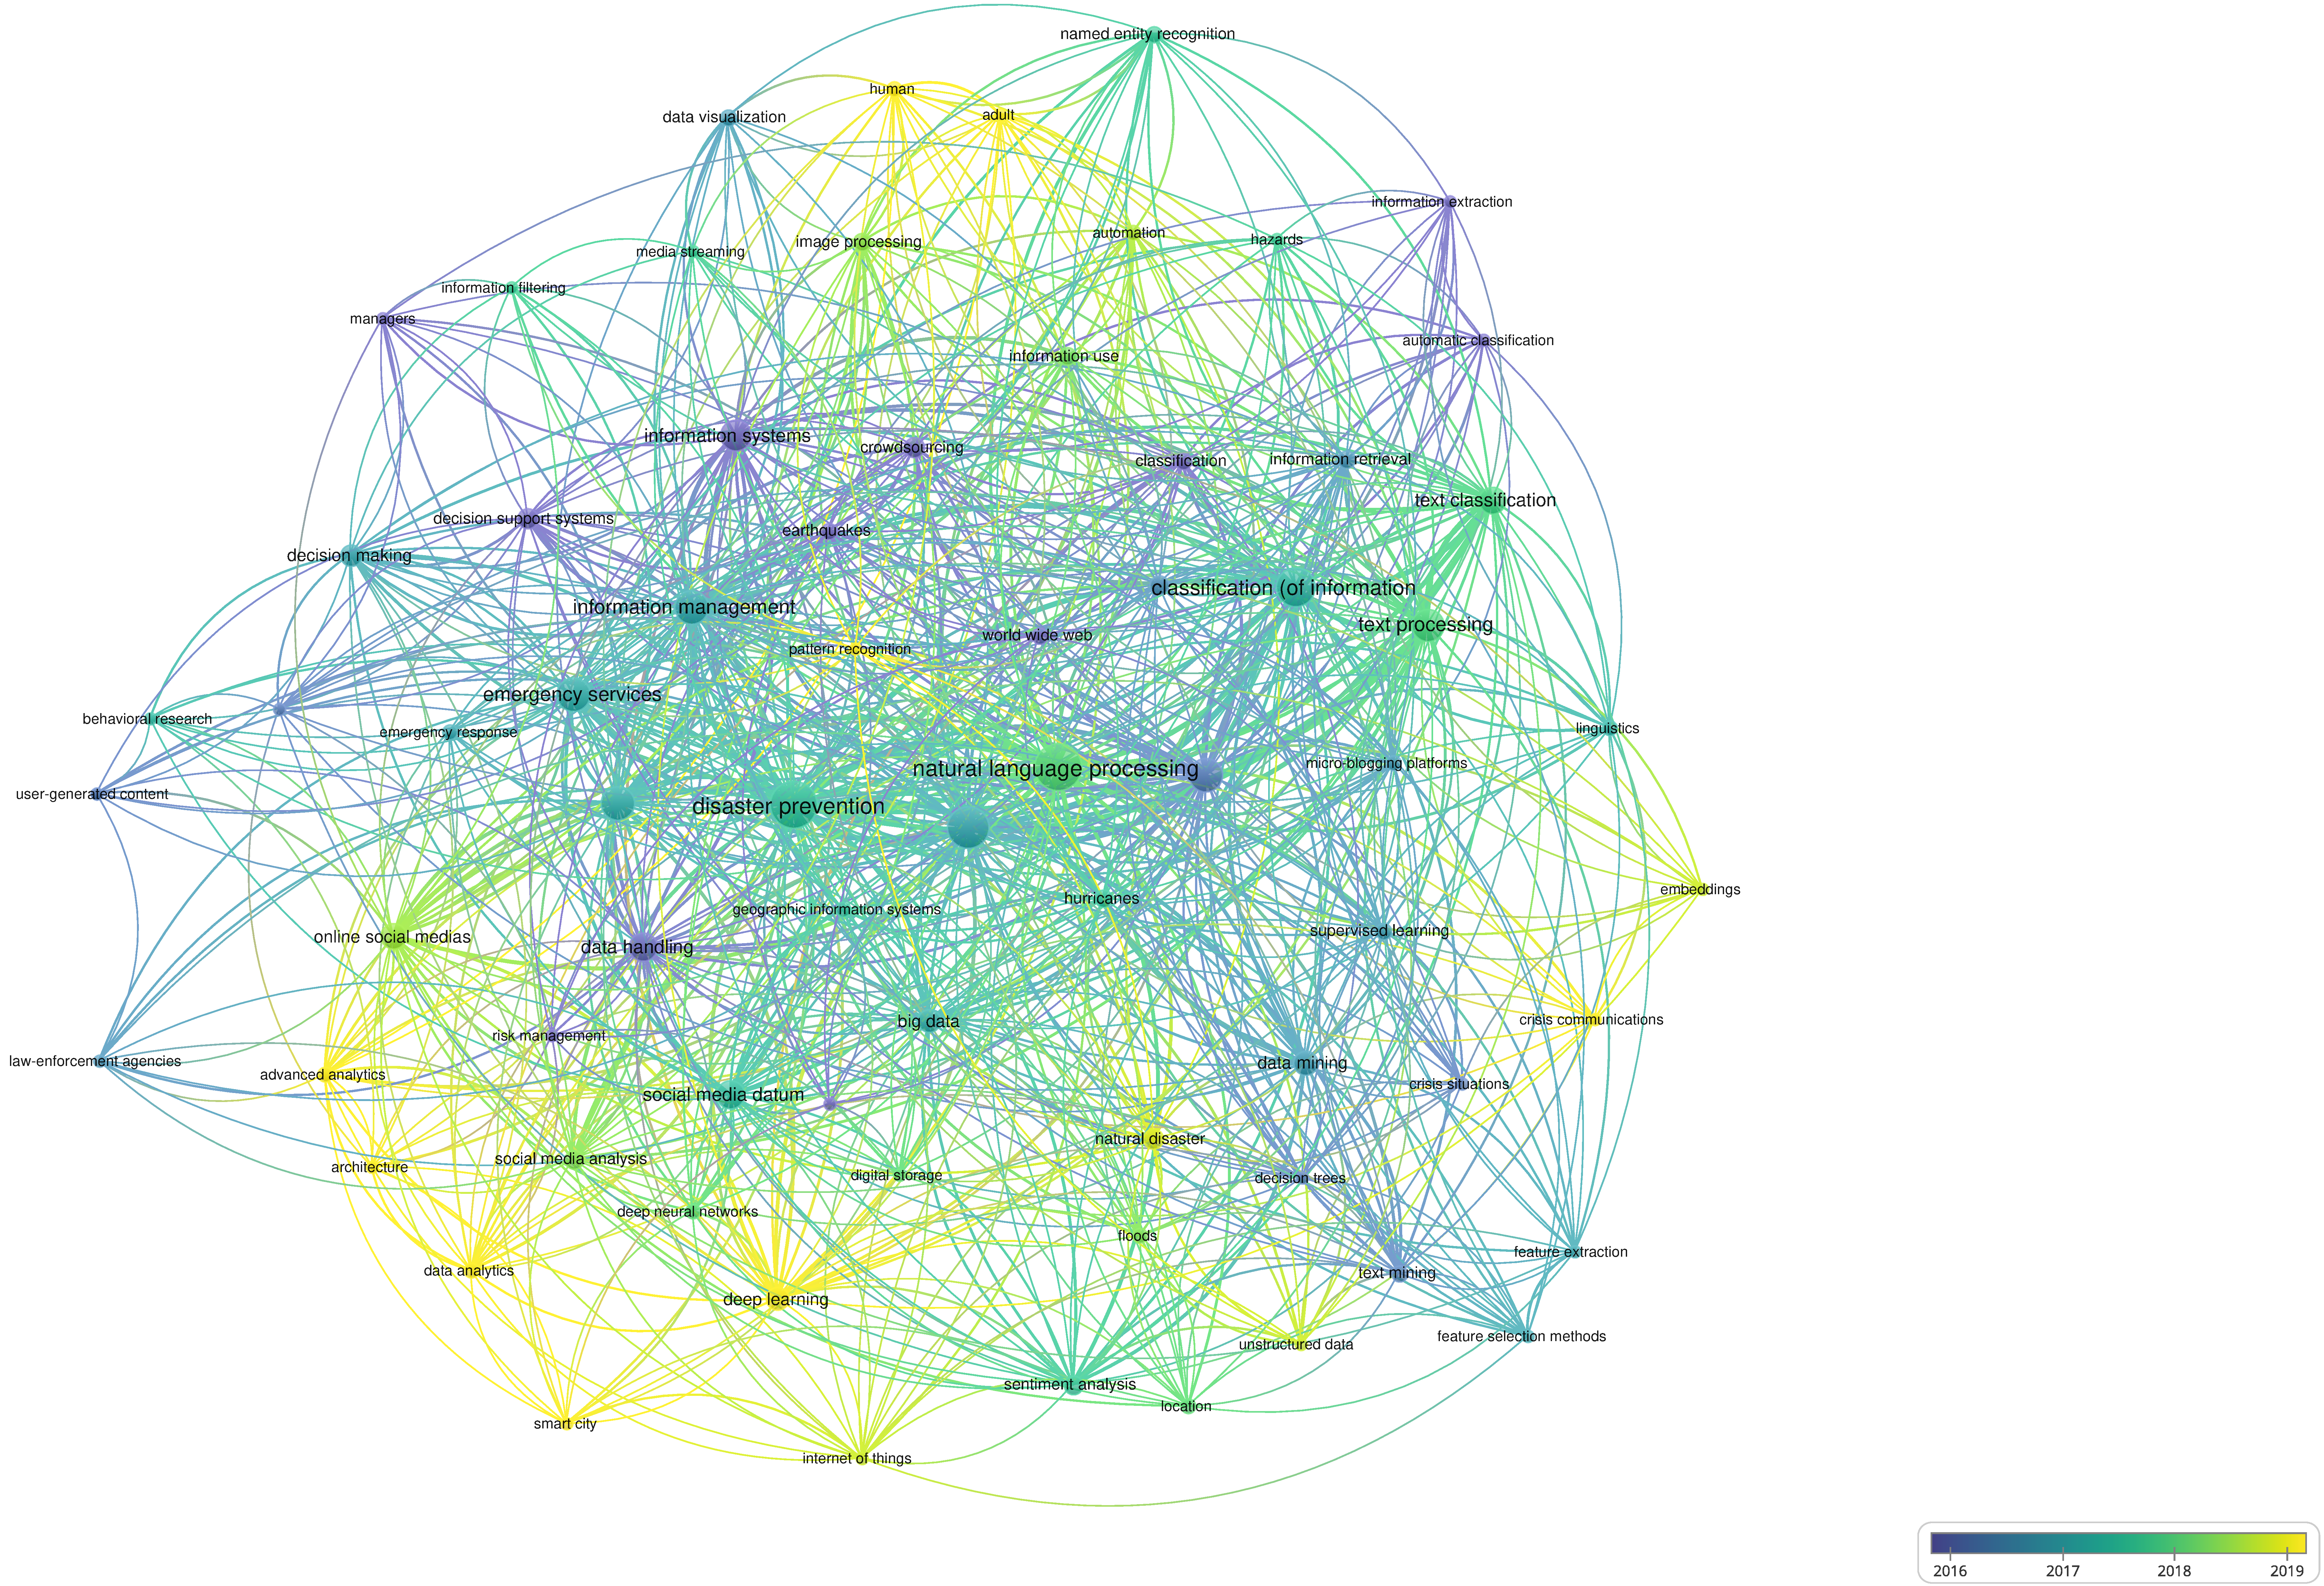
\includegraphics[width=\paperwidth,height=\paperheight,keepaspectratio]{figures/chap-2/crisis-informatic-overlay.pdf}
        \caption{Distribution of keywords with more than 3 occurrences among the articles from the query on crisis informatics. }
        \label{literature:crisis-informatic-overlay}
    \end{figure}
\end{landscape}

The bar diagram (Figure~\ref{literature:crisis-informatic-bar}) provides a better representation of the distribution of the occurrences of the different keywords.
From the most common ones, two areas of interest seem to emerge.
The automatic processing of the data, mostly textual according to the use of "natural language processing" and "text processing" is no more important than the use of this automation.
"Disaster prevention", "situation awareness", "information management" and "emergency services" highlight the importance of the applications of the results.

\begin{figure}[htb]
    \includegraphics[width=\textwidth]{figures/chap-2/crisis-informatic-bar.pdf}
    \caption{Distribution of keywords with more than 3 occurrences among the articles from the query on crisis informatics. }
    \label{literature:crisis-informatic-bar}
\end{figure}

As mentioned in the first chapter, automatically processing the content of social media to extract information is a new and promising scientific venue.
Thus, many attempted to create systems to achieve this goal, proposing features to improve systems' usability.
Overview of the different attempts and their feature, to identify what have been done in this area.
Table~\ref{table:crisis-informatic-main-articles} presents the results of the previous query that mention a processing system that uses social media as a data source and that have been cited at least ten times are shown.
From these main systems, were extracted the main features presented by their authors.

Among the features identified, the trend towards automation observed earlier is still clear.
The first works present systems that use crowdsourcing to identify relevant information from messages posted on social media
(\cite{schulzCrisisInformationManagement2012a, backfriedOpenSourceIntelligence2012a, imranAIDRArtificialIntelligence2014b}).
The following works were interested in automating the previous tasks, presumably to reduce the dependence on human actors and to improve the processing of the important amount of data.
Problems related to the detection of occurence of events and their related information on social media, have been explored using different approaches (\cite{imranAIDRArtificialIntelligence2014b,middletonRealtimeCrisisMapping2014a,avvenutiEARSEarthquakeAlert2014a, gibsonCombiningBigSocial2014a}).
In parallel, experiments were conducted to identify the best ways to organize and disseminate the information obtained (\cite{middletonRealtimeCrisisMapping2014a,huangDisasterMapperCyberGISFramework2015a,avvenutiPullingInformationSocial2016a,grunder-fahrerTopicsTopicalPhases2018a}).
Building on its successes, the field has continued to develop by relying on other available data formats and in particular images (\cite{alamImage4ActOnlineSocial2017a,nguyenAutomaticImageFiltering2017a,agarwalCrisisDIASMultimodalDamage2020a}).
Beyond the data, new questions have emerged, following feedback from the emergency departments involved in the experiments.
The detection of sub-events and of the different concerns of the impacted population are added to the results of previous works (\cite{wuStreamExplorerMultiStageSystem2018a,raginiBigDataAnalytics2018a,grunder-fahrerTopicsTopicalPhases2018a}).
More recently, teams with a broader vision are interested in the integration of such systems within the connected city (\cite{shahDisasterResilientSmart2019a}).
The multiplication of sources and formats naturally leads to the need for unified processing methods for data and fusion of information obtained by the different channels (\cite{alamDescriptiveVisualSummaries2020a}).

\begin{table}[bp]
    \centering
    \renewcommand{\arraystretch}{1.5}
    \caption{Articles retrieved from the previous request which propose social media processing systems or methods with at least 10 citations.}
    \begin{tabular}{m{0.3\textwidth} m{0.2\textwidth} m{0.5\textwidth}}
        Reference                                        & Type of event studied & Features                                                 \\ [0.5ex]
        \toprule
        \cite{schulzCrisisInformationManagement2012a}    & None                  & Crowdsourcing                                            \\
        \cite{backfriedOpenSourceIntelligence2012a}      & None                  & Crowdsourcing, Automatic processing                      \\
        \cite{imranAIDRArtificialIntelligence2014b}      & None                  & Crowdsourcing, Information categories, Message filtering \\
        \cite{middletonRealtimeCrisisMapping2014a}       & None                  & Common Operational Picture, Location inference           \\
        \cite{avvenutiEARSEarthquakeAlert2014a}          & Earthquake            & Event detection                                          \\
        \cite{gibsonCombiningBigSocial2014a}             & None                  & Formal concept analysis, Rule-based method               \\
        \cite{glasgowOurGriefUnspeakable2014a}           & None                  & Death-related content detection                          \\
        \cite{huangDisasterMapperCyberGISFramework2015a} & None                  & Big Data, Common Operational Picture                     \\
        \cite{avvenutiPullingInformationSocial2016a}     & Earthquake, Flooding  & Event detection, Message filtering, Disaster management  \\
        \cite{alamImage4ActOnlineSocial2017a}            & None                  & Image processing, Infrastructure damage                  \\
        \cite{fersiniEarthquakeManagementDecision2017a}  & Earthquake            & Message filtering, Information management                \\
        \cite{nguyenAutomaticImageFiltering2017a}        & None                  & Image processing, De-duplication, Image filtering        \\
        \cite{raginiBigDataAnalytics2018a}               & Flooding              & Sentiment analysis                                       \\
        \cite{shahDisasterResilientSmart2019a}           & Earthquake, Tsunami   & Smart Cities, IoT integration                            \\
        \cite{grunder-fahrerTopicsTopicalPhases2018a}    & None                  & Topic modeling, Disaster management                      \\
        \cite{wuStreamExplorerMultiStageSystem2018a}     & None                  & Subevent detection, Clustering                           \\
        \cite{agarwalCrisisDIASMultimodalDamage2020a}    & None                  & Damage identification, Severity detection                \\
        \cite{alamDescriptiveVisualSummaries2020a}       & Hurricane             & Information fusion                                       \\
        \bottomrule
    \end{tabular}
    \label{table:crisis-informatic-main-articles}
\end{table}

%TODO Conclusion of the section

\section{Decision making in crisis situation: information needed}
This first part of the literature review tackles the first sub problematic: What information that can be obtained from social media is relevant to the decisiom makers in crisis response?
Its looks at answers at the question: \emph{what information is relevant to the decisiom makers in crisis response?}

Information are at the heart of the decision making process (references to the decision making processs + figure to summarize the whole process)
In order to make decisions, the decision maker will look for information on certain elements.
What are these information?

The first part of this literature review will look at different attempts to model the information needed in crisis response, from a decision maker point of view.
This part only consider the models that consider in their scope the stakes of crisis management identified in the first chapter: improve coordination and/or situational awareness.

\subsection{Information identified for crises: crisis situation models}
Crisis management is not a novel issue.
Thus, many tackled the problems in this area.
With the apparition of informatic as a way to delegate tasks, many thought about deligating a part of crisis management to the machine.
However, managing this information require at first to build representations of the crises for the computers.
Consequently, ontologies and information models emerged to represent the informational concepts manipulated during an emergency situation.
This sub-section aims at retrieving from the literature the different key informational concepts, useful for decision makers during crisis response.

The request run on Scopus is as follow:
\begin{itemize}
    \item SUBJAREA(comp)
    \item AND (TITLE-ABS-KEY ({crisis management} or {crisis response} or {disaster management} or contingency or {disaster response}))
    \item AND (TITLE-ABS-KEY (ontology or metamodel))
    \item AND (EXCLUDE (DOCTYPE,"re") OR EXCLUDE (DOCTYPE,"cr"))
\end{itemize}

The request returns papers that:
\begin{itemize}
    \item Are in the computer science domain, as this domain contains both the AI and Information Systems domains.
    \item Are centered around crises|disasters management|response or contingency plans.
    \item That present systems that process data
    \item Papers that present conference tracks and reviews are excluded.
\end{itemize}

The request returns 205 documents, published between 1998 and 2021.
Figure~\ref{literature:situation-models-hist} shows the evolution of the volume of publication between 1998 and 2020.
The field has emerged around 2000 and built momentum during ten years to reach a plateau of fifteen articles on average per years.
The domain developped in order to organize the data, information and knowledge present during crisis events.
To achieve this goal, representions of the different concepts involved during such events were needed.
Two paths to represent these concepts have been taken: ontologies and metamodels.
Ontologies and metamodels are very close concepts.
Both methods aim at creating a controlled vocabulary to define the entities and their relations in a given domain.
The difference between the two methos happens at the grammar used for the vocabulary.
Metamodels usually use a formal and common grammar (a modelisation language such as UML) to ease the distribution and development of these representation.
Metamodels, as the backbone of model driven engineering, tend to be developped with interoperability between different systems in mind.
Thus the use of common tools to represent concepts between the engineers.
Ontologies, on the other hand, use their own grammar for the entities that its define.
As mentioned in the first chapter, crises are a were wide concept and the creation of ontologies or metamodels of crisis situations is a very challenging task.
Thus, many ontologies and metamodels have been created to represent different aspects of crisis management.

\begin{figure}[htb]
    \includegraphics[width=\textwidth]{figures/chap-2/situation-models-hist.pdf}
    \caption{Timelime of the volume of contributions per years for the crisis-situation models domain. The year 2021 is excluded because the year is not complete at the time of writing.}
    \label{literature:situation-models-hist}
\end{figure}

Following the same methodology as in the previous section, Figure~\ref{literature:situation-models-overlay} provides a visual of the evolution over time of the different keywords used in the fetched articles.
The overlay indicates three clusters: a major one and two smaller ones.
One is related to genes and the other one is related to supply chains and infrastructures.
The one related to genes is a cluster of outliers, composed of 7 articles from the medical field.
The second cluster is also composed of few articles centered around ontologies for the petroleum sector.
The main cluster however, is more centered on the topic of this literature review.
As in the previous section, the evolution (represented by the color variation) of the keywords hint at the direction of the domain over time.

\begin{landscape}
    \begin{figure}[htb]
        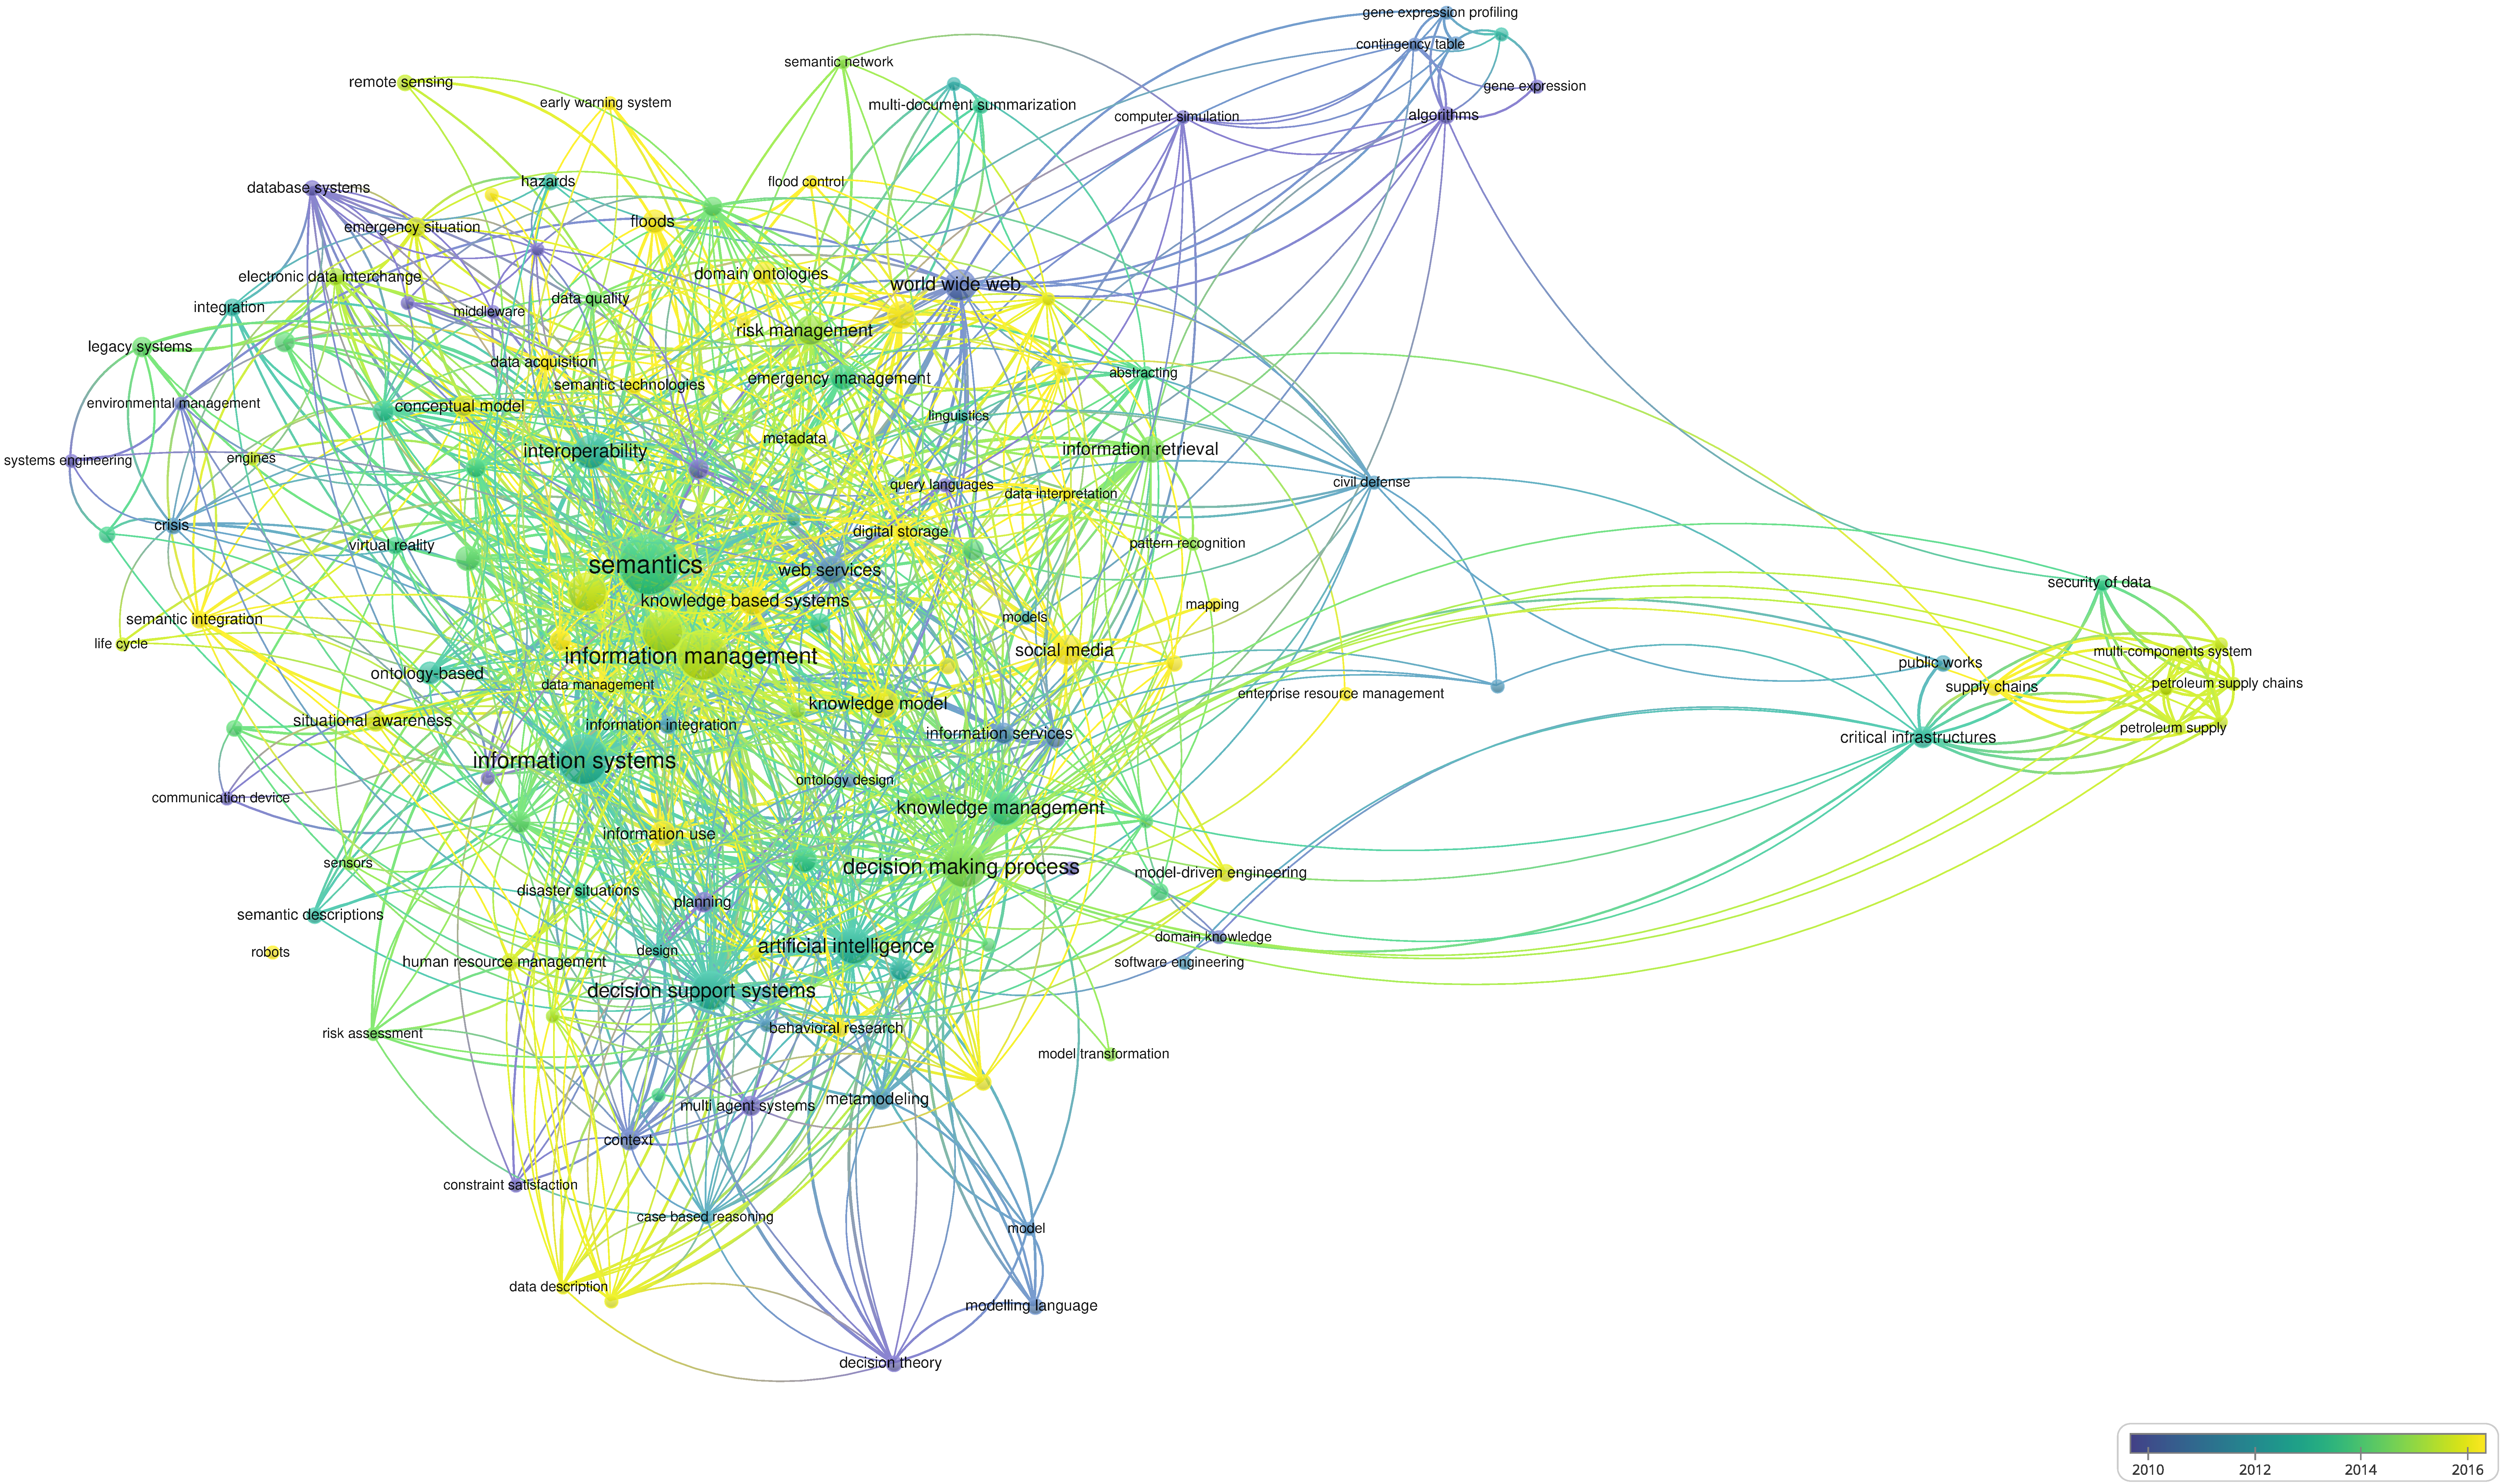
\includegraphics[width=\paperwidth,height=\paperheight,keepaspectratio]{figures/chap-2/situation-models-overlay.pdf}
        \caption{Distribution of keywords with more than 3 occurrences among the articles from the query on crisis-situation models.}
        \label{literature:situation-models-overlay}
    \end{figure}
\end{landscape}

Unlike the query, the overlay spans from 2010 to 2016. This is because the overlay does not include all keywords, but only those that appear in at least 3 different articles.
By cross-checking this information with the previous histogram, one understands the reason for this short period.
For many years the number of publications was relatively low, and apparently without any real consensus among the keywords.
If this is understandable at the beginning of a field, this explanation does not explain the stop of the overlay from 2016.
However, using again the histogram, one notices that the domain loses popularity from 2015 onwards to return to its previous level around 2018.
It is possible to hypothesize that it is this loss of interest that has led to the result observed on the overlay.

Despite this short span covered, it is possible to identify trends in keywords use somehow similar to the ones in crisis informatic.
The older keywords used, such as "SOA", "simulation", "multi agent systems" and "systems engineering" show an interest centered around the core of what were used ontologies and metamodels for: model driven engineering and information management.
Then, the field knew a pic of interest, as the previous histogram show.
This period reflects on Figure~\ref{literature:situation-models-bar}, where one can observe that most of the most importants keywords are located between 2012 and 2014.
As explained previously, the years between 2021 and 2014 were indeed the most prolific.
These years were mostly focused on the idea of crisis management systems, powered by artifical intelligence for decision support.
Artificial intelligence would automatically create the information representations needed by systems.
As these representations would have been written in a common fashion, these systems would have been able to quickly adapt to new representations, providing greater interoperability.
After this period, the interest in the field decrease a few, before coming back with new approaches.
Knowledge based systems and knowledge management started to appear, as well as a reborn of metamodel and ontologies creation, powered by improvements in machine learning.

\begin{figure}[htb]
    \includegraphics[width=\textwidth]{figures/chap-2/situation-models-bar.pdf}
    \caption{Distribution of keywords with more than 4 occurrences among the articles from the query on crisis-situation models.}
    \label{literature:situation-models-bar}
\end{figure}

In association with the previous qualitative review of the field, Table~\ref{table:situation-models-main-articles} presents the decision makers needs identified in the articles from the previous request with at least 25 citations.
Duplicates and unrelated articles (e.g. gene ontologies) are also excluded.
This review of the main articles highlight the diversity of approaches covered by ontologies and metamodels.
Some of these ontologies are event specific (\cite{xuModelingRepresentationEarthquake2014a,qiuIntegratedFloodManagement2017a,jungOntologydrivenSlopeModeling2015a}).
While these models are effective at dealing with the event they are designed for, most of their concept representations do not fit with other kind of events.

Collaboration between the actors is, as presented in the introductory chapter, a matter of interest for crisis management organizations.
Thus (\cite{benabenMetamodelItsOntology2008b}) and (\cite{othmanDevelopmentValidationDisaster2014b}) propose metamodels to represent the collaboration between several actors, independantly of the type of crisis.

Others have also focused on emergency organization and proposed ways to improve their functioning.
\cite{chouOntologyDevelopingWeb2011a} proposed a way to automatically create websites to dissemination information related to an ongoing event.
As reports are an important concerns and participate to information overload, \cite{liOntologyenrichedMultiDocumentSummarization2010a} created an ontology to assist in report summarization.
Disaster management software are inherently complex. Thus, \cite{babitskiSoKNOSUsingSemantic2011a} proposed an ontology to assist in their development and another to assess their functionalities.
As disaster management systems grow, they become intricated and complex. \cite{madniSystemsIntegrationKey2014a} proposed an ontology to facilitate their integration into a functioning system of systems.

All the systems mentioned above require data.
Fortunately, sensors are excellent ways to keep emergency responders informed of certain caracteristics of their environment.
\cite{posladSemanticIoTEarly2015a} and \cite{babitskiOntologybasedIntegrationSensor2009a} proposed ontologies to better integrate sensors data into crisis cells.
Finally, another type of sensor considered are humans, acting as social sensors whose data can be automatically gathered from social media plateforms.
\cite{purohitIdentifyingSeekersSuppliers2014a} proposed an ontology to identify victims requests and volunteers capabilities from tweets.
As being able to geolocate the individual behind a post allows better actionability for emergency services, \cite{ghahremanlouGeotaggingTwitterMessages2014a} built an ontology to help solve this issue.

\begin{table}[bp]
    \centering
    \renewcommand{\arraystretch}{1.5}
    \caption{Articles retrieved from the previous request which propose social media processing systems or methods with at least 25 citations.}
    \begin{tabular}{m{0.25\textwidth} m{0.75\textwidth}}
        Reference                                                & Decision makers needs adressed         \\ [0.5ex]
        \toprule
        \cite{benabenMetamodelItsOntology2008b}                  & Collaboration                          \\
        \cite{babitskiOntologybasedIntegrationSensor2009a}       & Sensor integration                     \\
        \cite{liOntologyenrichedMultiDocumentSummarization2010a} & Reports summarization                  \\
        \cite{babitskiSoKNOSUsingSemantic2011a}                  & Disaster management software usability \\
        \cite{chouOntologyDevelopingWeb2011a}                    & Automatic web sites creation           \\
        \cite{ghahremanlouGeotaggingTwitterMessages2014a}        & Location retrieval                     \\
        \cite{madniSystemsIntegrationKey2014a}                   & System integration                     \\
        \cite{othmanDevelopmentValidationDisaster2014b}          & Collaboration                          \\
        \cite{purohitIdentifyingSeekersSuppliers2014a}           & Identify victims and volunteers        \\
        \cite{xuModelingRepresentationEarthquake2014a}           & Earthquake management                  \\
        \cite{jungOntologydrivenSlopeModeling2015a}              & Landslide prevention                   \\
        \cite{posladSemanticIoTEarly2015a}                       & Sensor intregration                    \\
        \cite{qiuIntegratedFloodManagement2017a}                 & Flood management                       \\
        \bottomrule
    \end{tabular}
    \label{table:situation-models-main-articles}
\end{table}

This part identified the different approaches to model information in crisis response from a decision maker point of view.
Yet, most of these approaches are top-down, and few conducted interviews to directly identify decision makers needs'.
The next section looks at articles in the literature that used a bottom-up approach to identify the aforementioned needs.

\subsection{Information needs of emergency services}
Emergency management teams have special have special information needs.
Sociologists have been interested in these needs and have conducted interviews to identify and understand what information is needed.
This section aims to highlight the main needs identified in the literature.

The executed request is:

\begin{itemize}
    \item TITLE-ABS-KEY({information gathering} or interview?)
    \item AND TITLE-ABS-KEY({emergency responders} or {Emergency services} or {dispatchers})
    \item AND (LIMIT-TO (SUBJAREA,"SOCI") OR LIMIT-TO (SUBJAREA,"COMP") OR LIMIT-TO (SUBJAREA,"DECI"))
    \item AND (EXCLUDE(DOCTYPE,"re") OR EXCLUDE(DOCTYPE,"cr"))
\end{itemize}

It aims at obtaining articles that:

\begin{itemize}
    \item Mention information gathering or interview in their content and mention emergency responders, dispatchers or emergency services.
    \item Are linked to social sciences, computer sciences or decision sciences.
    \item Papers that present conference tracks and reviews are excluded.
\end{itemize}

The request returns 219 documents, published between 1995 and 2021.
The area follows an increasing trend similar to the other two previous areas.
Interest in the study of emergency services has been growing rapidly since the 2000s.
This interest grew relatively steadily until today, where about 20 articles are published per year on the subject (Figure~\ref{literature:business-needs-hist}).

\begin{figure}[htb]
    \centering
    \includegraphics[width=\textwidth]{figures/chap-2/business-needs-hist.pdf}
    \caption{Timelime of the volume of contributions per years for information needs of crisis responders. The year 2021 is excluded because the year is not complete at the time of writing.}
    \label{literature:business-needs-hist}
\end{figure}

The overlay of the keywords generated from the articles retrieved (Figure~\ref{literature:business-needs-overlay}) spans from 2010 to 2018.
It reveals two clusters: one centered on medical issues and another one centered on information systems.
The medical cluster is mainly focused on the well-being of the personnel in charge of the emergency and in particular in their psychological health.
The other cluster is more focused on the information systems of emergency services and in the management of events.
This last one being more in connection with the objective of this manuscript, the next analysis will be focused on it.

\begin{landscape}
    \begin{figure}[htb]
        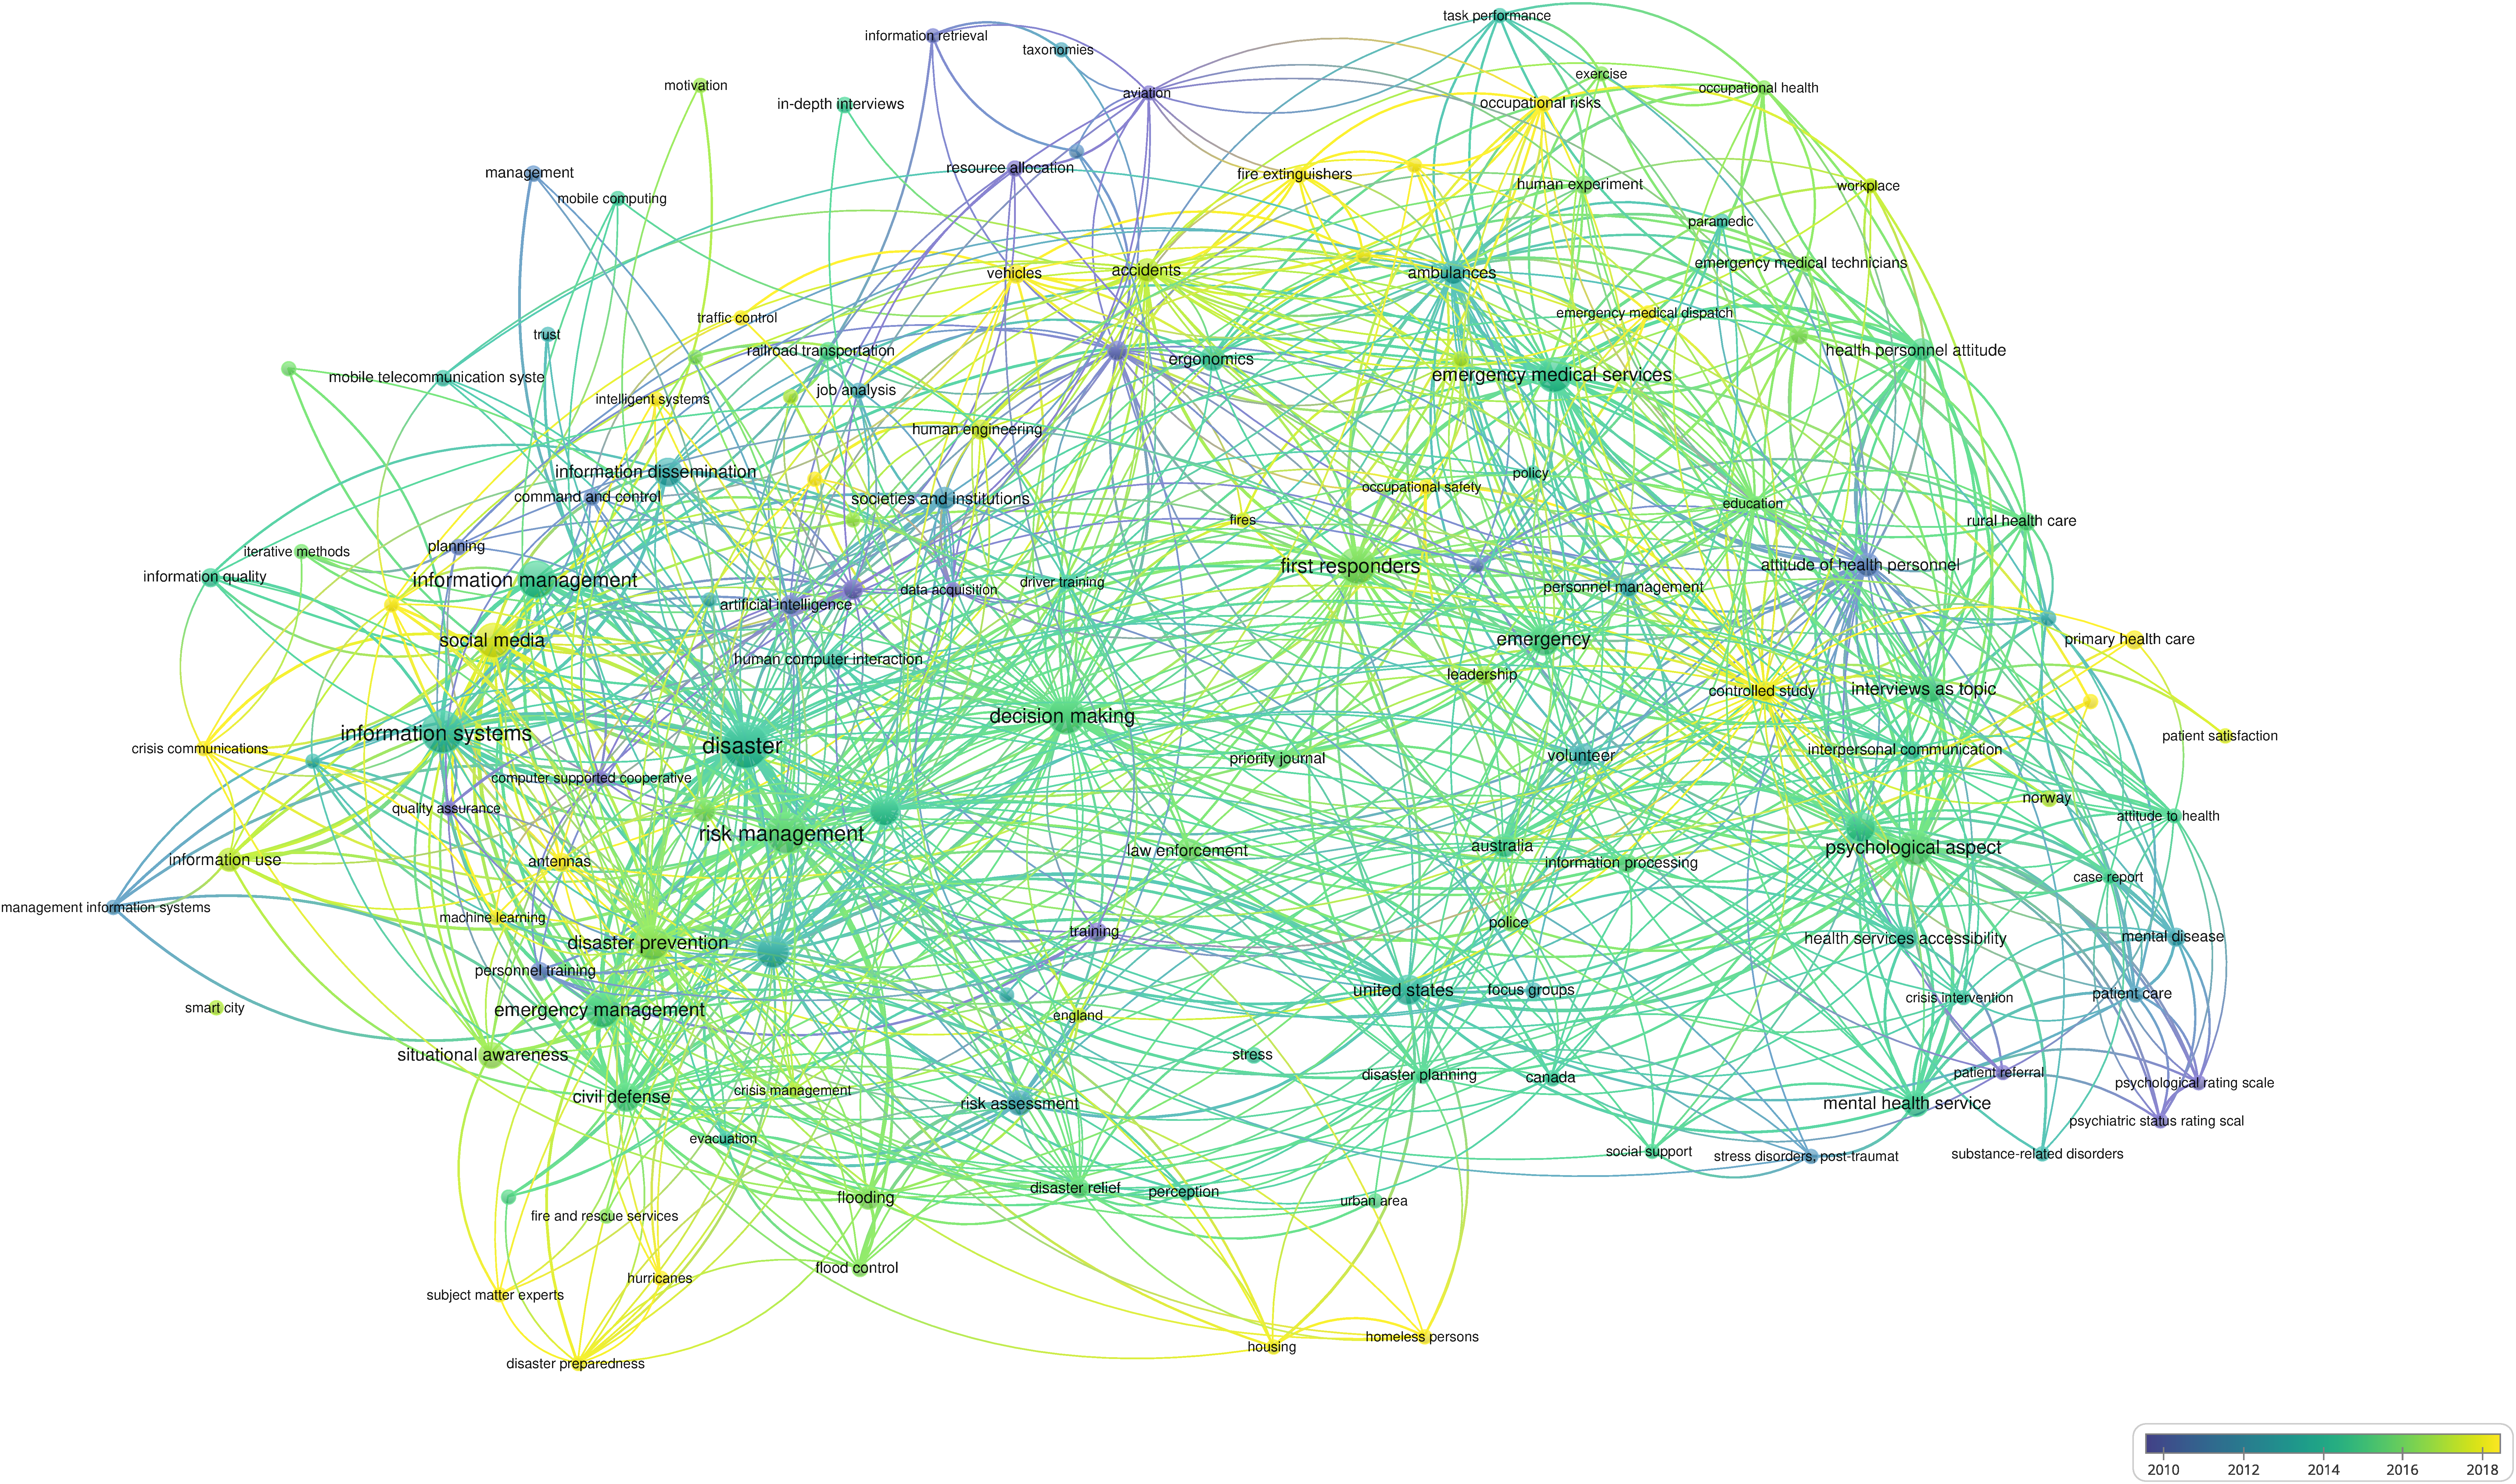
\includegraphics[width=\paperwidth,height=\paperheight,keepaspectratio]{figures/chap-2/business-needs-overlay.pdf}
        \caption{Distribution of keywords with more than 3 occurrences among the articles from the query on information needs of crisis responders.}
        \label{literature:business-needs-overlay}
    \end{figure}
\end{landscape}

The left cluster is composed of the most common keywords used in the fetched articles.
Keywords such as \emph{disaster}, \emph{information systems} and \emph{risk management} (Figure~\ref{literature:business-needs-bar}) are the most prominent ones and seems to be mostly used circa 2014.
Prior to that period (between 2010 and 2014), the field was mostly focusing on planification of resources and training.
But the field took a shift towards data processing to support \emph{decision making} during emergency events.
The collision with the other domains explored in this chapter seems to happen around 2018, were keywords such as \emph{machine learning}, \emph{social media} or \emph{situational awareness}.

\begin{figure}[htb]
    \centering
    \includegraphics[width=\textwidth]{figures/chap-2/business-needs-bar.pdf}
    \caption{Distribution of keywords with more than 3 occurrences among the articles from the query on information needs of crisis responders.}
    \label{literature:business-needs-bar}
\end{figure}

Table~\ref{table:business-needs-main-articles} provides a summary of the responders need identified in the most prominent articles in the field.
Articles were selected if they had at least 25 citations, have been published in 2010 or after, are located in the information systems cluster and are not duplicates.
The articles retrieved provide insights on what are some of the pain points of emergency organizations.

Some studies are event specific, due to a governemental request or a gap in the emergency preparation cover.
\textcite{lindellTsunamiPreparednessOregon2010a} is interested in tsunamis management on the US east coast and \textcite{cabreraaguileraModellingPerformanceVariabilities2016a} tackle oil spill.
Both studies do not address any particular point in the management of this type of event.
Rather, they implement the entire crisis management cycle for these events, which were not considered until their work.
Unfortunately, no specific information need for decision-makers emerges.

On the other hand, others articles are most focused on specific needs of emergency organizations.
Collaboration, information sharing and joint preparation exercices are one of the concerns raised \parencite{berlinWhyCollaborationMinimised2011a,parkerSurfaceWaterFlood2011a}.
The increasing complexity of crisis events ask for a wider range of skills.
As no organization can possess all the required skills at the same time, other actors have to be involved.
Crisis management organization acknowledge that an unexpected collaboration between actors yield poor outcomes during the response.
Thus, exercices and discussions are key during the preparation phase and an adequate means of communication between the actors during the response are needs identified by the studies.

\textcite{yangDesignPrinciplesIntegrated2012a} highlight an interesting and well mentioned need for crisis response: situation awareness.
Situation awareness correspond to the representation of the state of the environment that surround the emergency response organization during an event.
This representation directly guides decision making.
Consequently, building the best and most accurate representation possible directly at the start of the event is critical.
In there are articles, \citeauthor{yangDesignPrinciplesIntegrated2012a} emphasize 4 critical pieces of information for situational awareness:

\begin{enumerate}
    \item Environmental conditions such as the building infrastructure, number of occupants, and the exact location of any hazard;
    \item Information on the response participants such as who is involved in the response, what skills they could offer, and what resources they bring to the scene;
    \item The status of any casualties, the accident location, cause, and severity; and
    \item The available resources including equipment and food.
\end{enumerate}

As per the authors, "timeliness, accuracy, and completeness are the critical dynamic attributes of these four categories of information".
The next chapter (chapter 3) will dive deeper into this concept.

The issue with building an accurate situation awareness is the need for information.
With the disruption of the regular means of communication and information channels, decison makers are shrouded in darkness.
According to \textcite{tapiaTrustworthyTweetDeeper2013a,cobbDesigningDelugeUnderstanding2014a}, some emergency centers acknowledge the benefit of social media as a potential information source.
However, the issue identified is the lack of tools and methods, similar to the ones that built for calls, for social media.

Finally, the last need identified among the extracted items is the communication to the public.
\textcite{aloudatRegulationUbiquitousMobile2011a} insist on the potential yielded by modern communication means such as cell phones and social media to share information with the public during an event.
As people are not always around a radio or a TV, they often miss critical messages during fast moving events (floods, fires...), resulting in casualties.
On the other hand, (almost literally) most of the population carry a cellphone nowadays, and the critical messages could be distributed faster and with a better viewing rate than traditional methods.
Text messages or notifications from social media could be more effective communication channels that emergency response teams should use.

\begin{table}[bp]
    \centering
    \renewcommand{\arraystretch}{1.5}
    \caption{Articles on informational needs of emergency responders retrieved from the previous request with at least 25 citations.}
    \begin{tabular}{m{0.25\textwidth} m{0.75\textwidth}}
        Reference                                                    & Business need identified by the authors.                                                                                                                                                                               \\ [0.5ex]
        \toprule
        \cite{lindellTsunamiPreparednessOregon2010a}                 & Tsunami training                                                                                                                                                                                                       \\
        \cite{aloudatRegulationUbiquitousMobile2011a}                & Communication to the public                                                                                                                                                                                            \\
        \cite{berlinWhyCollaborationMinimised2011a}                  & Collaboration between the different actors                                                                                                                                                                             \\
        \cite{parkerSurfaceWaterFlood2011a}                          & Create conversations between unusual actors during the preparation phase                                                                                                                                               \\
        \cite{yangDesignPrinciplesIntegrated2012a}                   & Increase situation awareness, Identify key informations~\footnote{(hazard environment, information concerning the responder workforce, information on evolving safety issues, and information about safety equipment)} \\
        \cite{tapiaTrustworthyTweetDeeper2013a}                      & Accounting for informal sources of data (such as social media)                                                                                                                                                         \\
        \cite{cobbDesigningDelugeUnderstanding2014a}                 & Big data processing methods adapted to social media data                                                                                                                                                               \\
        \cite{cabreraaguileraModellingPerformanceVariabilities2016a} & Oil spill preparation                                                                                                                                                                                                  \\
        \bottomrule
    \end{tabular}
    \label{table:business-needs-main-articles}
\end{table}

In concl

\subsection{Information needs: place of social media?}
Looking back at the first chapter, the sub problematic linked to this section was: \emph{What information that can be obtained from social media is relevant to the decisiom makers in crisis response?}
The two previous subsections identified several references that explored the information needs of decision makers in crisis management.
Each sub-section respectively explored top-down and bottom-up approaches.
However, social media were not directly considered in the query made on the bibliographic database as social media are not the only concern of these fields.

This sub-section emphasize on the intersection of the previous results and social media.
Crisis situation models:
Among the 205 documents on crisis situation models, 22 articles include the keywords \emph{social media} or \emph{twitter} to the query.
Two articles from the list of articles qualified as prominent are centered on social media:

\begin{itemize}
    \item \textcite{purohitIdentifyingSeekersSuppliers2014a}
    \item \textcite{ghahremanlouGeotaggingTwitterMessages2014a}
\end{itemize}

The same approach applied to the needs of crisis management organizations provides a similar number of articles.
22 articles among the 219 mention \emph{social media} or \emph{twitter}.
Among the articles studied in the previous part, two are dedicated to social media:

\begin{itemize}
    \item \textcite{cobbDesigningDelugeUnderstanding2014a}
    \item \textcite{tapiaTrustworthyTweetDeeper2013a}
\end{itemize}

In both cases, only roughly 10\% of the total body of surveys mention social media.
% From the remaining articles, most of the ontologies or metamodels are studied and represent information flows during an event.
% For instance, \textcite{montarnalAutomatedEmergenceCrisis2017a} create an ontology to merge data coming from social media and sensors.
% \textcite{gaurEmpathiOntologyEmergency2019a} followed up by adding satellites images.
% It appears that the information available during the event and the management of the same event are too different to get associated in the same representation.
% Despite this explanation, very few link the two to create a representation of emergency management mindful of the information available.

This section was answering the question: \emph{what information is relevant to the decisiom makers in crisis response?}
Many studied this question and this section explored two ways taken by two research communities to answer this question.
These two ways correspond to the two subsections.
The first sub-section was dedicated to model engineering and the previous attempts to create representations or abstractions to represent the concepts involved in an emergency.
This approach is fed by the need of automation of certain tasks in crisis management, hence the need of concepts to represent and manage the different aspects.
However, this approach is essentially top-down, and few references actually report feedbacks from field interviews.

This insight feeds the need to gather the information requirements of the primary users during their operations.
Hence, the second sub-section, dedicated to the report of these information requirements gathered through interviews.
Yet, this bottom-up approach is unstructured, and the results would need additional work to get integrated in an automation system.

Overall, the information needs identified are:

\begin{itemize}
    \item Situation Awareness
    \item Collaboration
    \item Communication to the public
    \item Social media accounting
    \item Sensor data integration
    \item Large data volume processing
\end{itemize}

The next section will be dedicated to the existing ways of identifying and mining information from social media, in order to later retrieve the previous information.

\section{NLP tools for information extraction from social media data}
The first chapter presented the NLP domain.
Through its development, many tools have been developed to process textual data.
With the emergence of social media, a new source of textual data appeared.

Part 1 presents the goals of applications of NLP for social media data.

Part 2 presents

This section is broken down into two parts.
The first one asks the question: What kind of information can NLP on social media data extracts?
The second question is: How the previous information can be extracted ?
This sections asks the question: How the content of social media can be processed to deliver information?
It can be decomposed according to the three kinds of AI: rule based, statistic based and deep neural network based.

\subsection{Social media information extracted using NLP}
Social media data is used as a data source in a various of use cases.
The following request provides some insights on the use cases:
\begin{itemize}
    \item (TITLE-ABS-KEY({natural language processing} or {information mining}))
    \item AND (TITLE-ABS-KEY({social media} or Twitter))
    \item AND (TITLE-ABS-KEY(survey))
\end{itemize}
Synonyms have been aggregated, keywords from the query removed and keywords such as "state of the art, large amounts, codes (symbols), research questions, text".
The Figure machine provides an overview of the major keywords return by the request.

Figure~\ref{literature:nlp-hist}

\begin{figure}[bp]
    \centering
    \includegraphics[width=\textwidth]{figures/chap-2/nlp-hist.pdf}
    \caption{Timelime of the volume of contributions per years for the crisis informatic domain. The year 2021 is excluded because the year is not complete at the time of writing.}
    \label{literature:nlp-hist}
\end{figure}

Figure~\ref{literature:nlp-bar}

\begin{figure}[bp]
    \centering
    \includegraphics[width=\textwidth]{figures/chap-2/nlp-bar.pdf}
    \caption{Distribution of keywords with more than 3 occurrences among the articles from the query on crisis informatics. }
    \label{literature:nlp-bar}
\end{figure}

Figure~\ref{literature:nlp-overlay}

\begin{figure}[bp]
    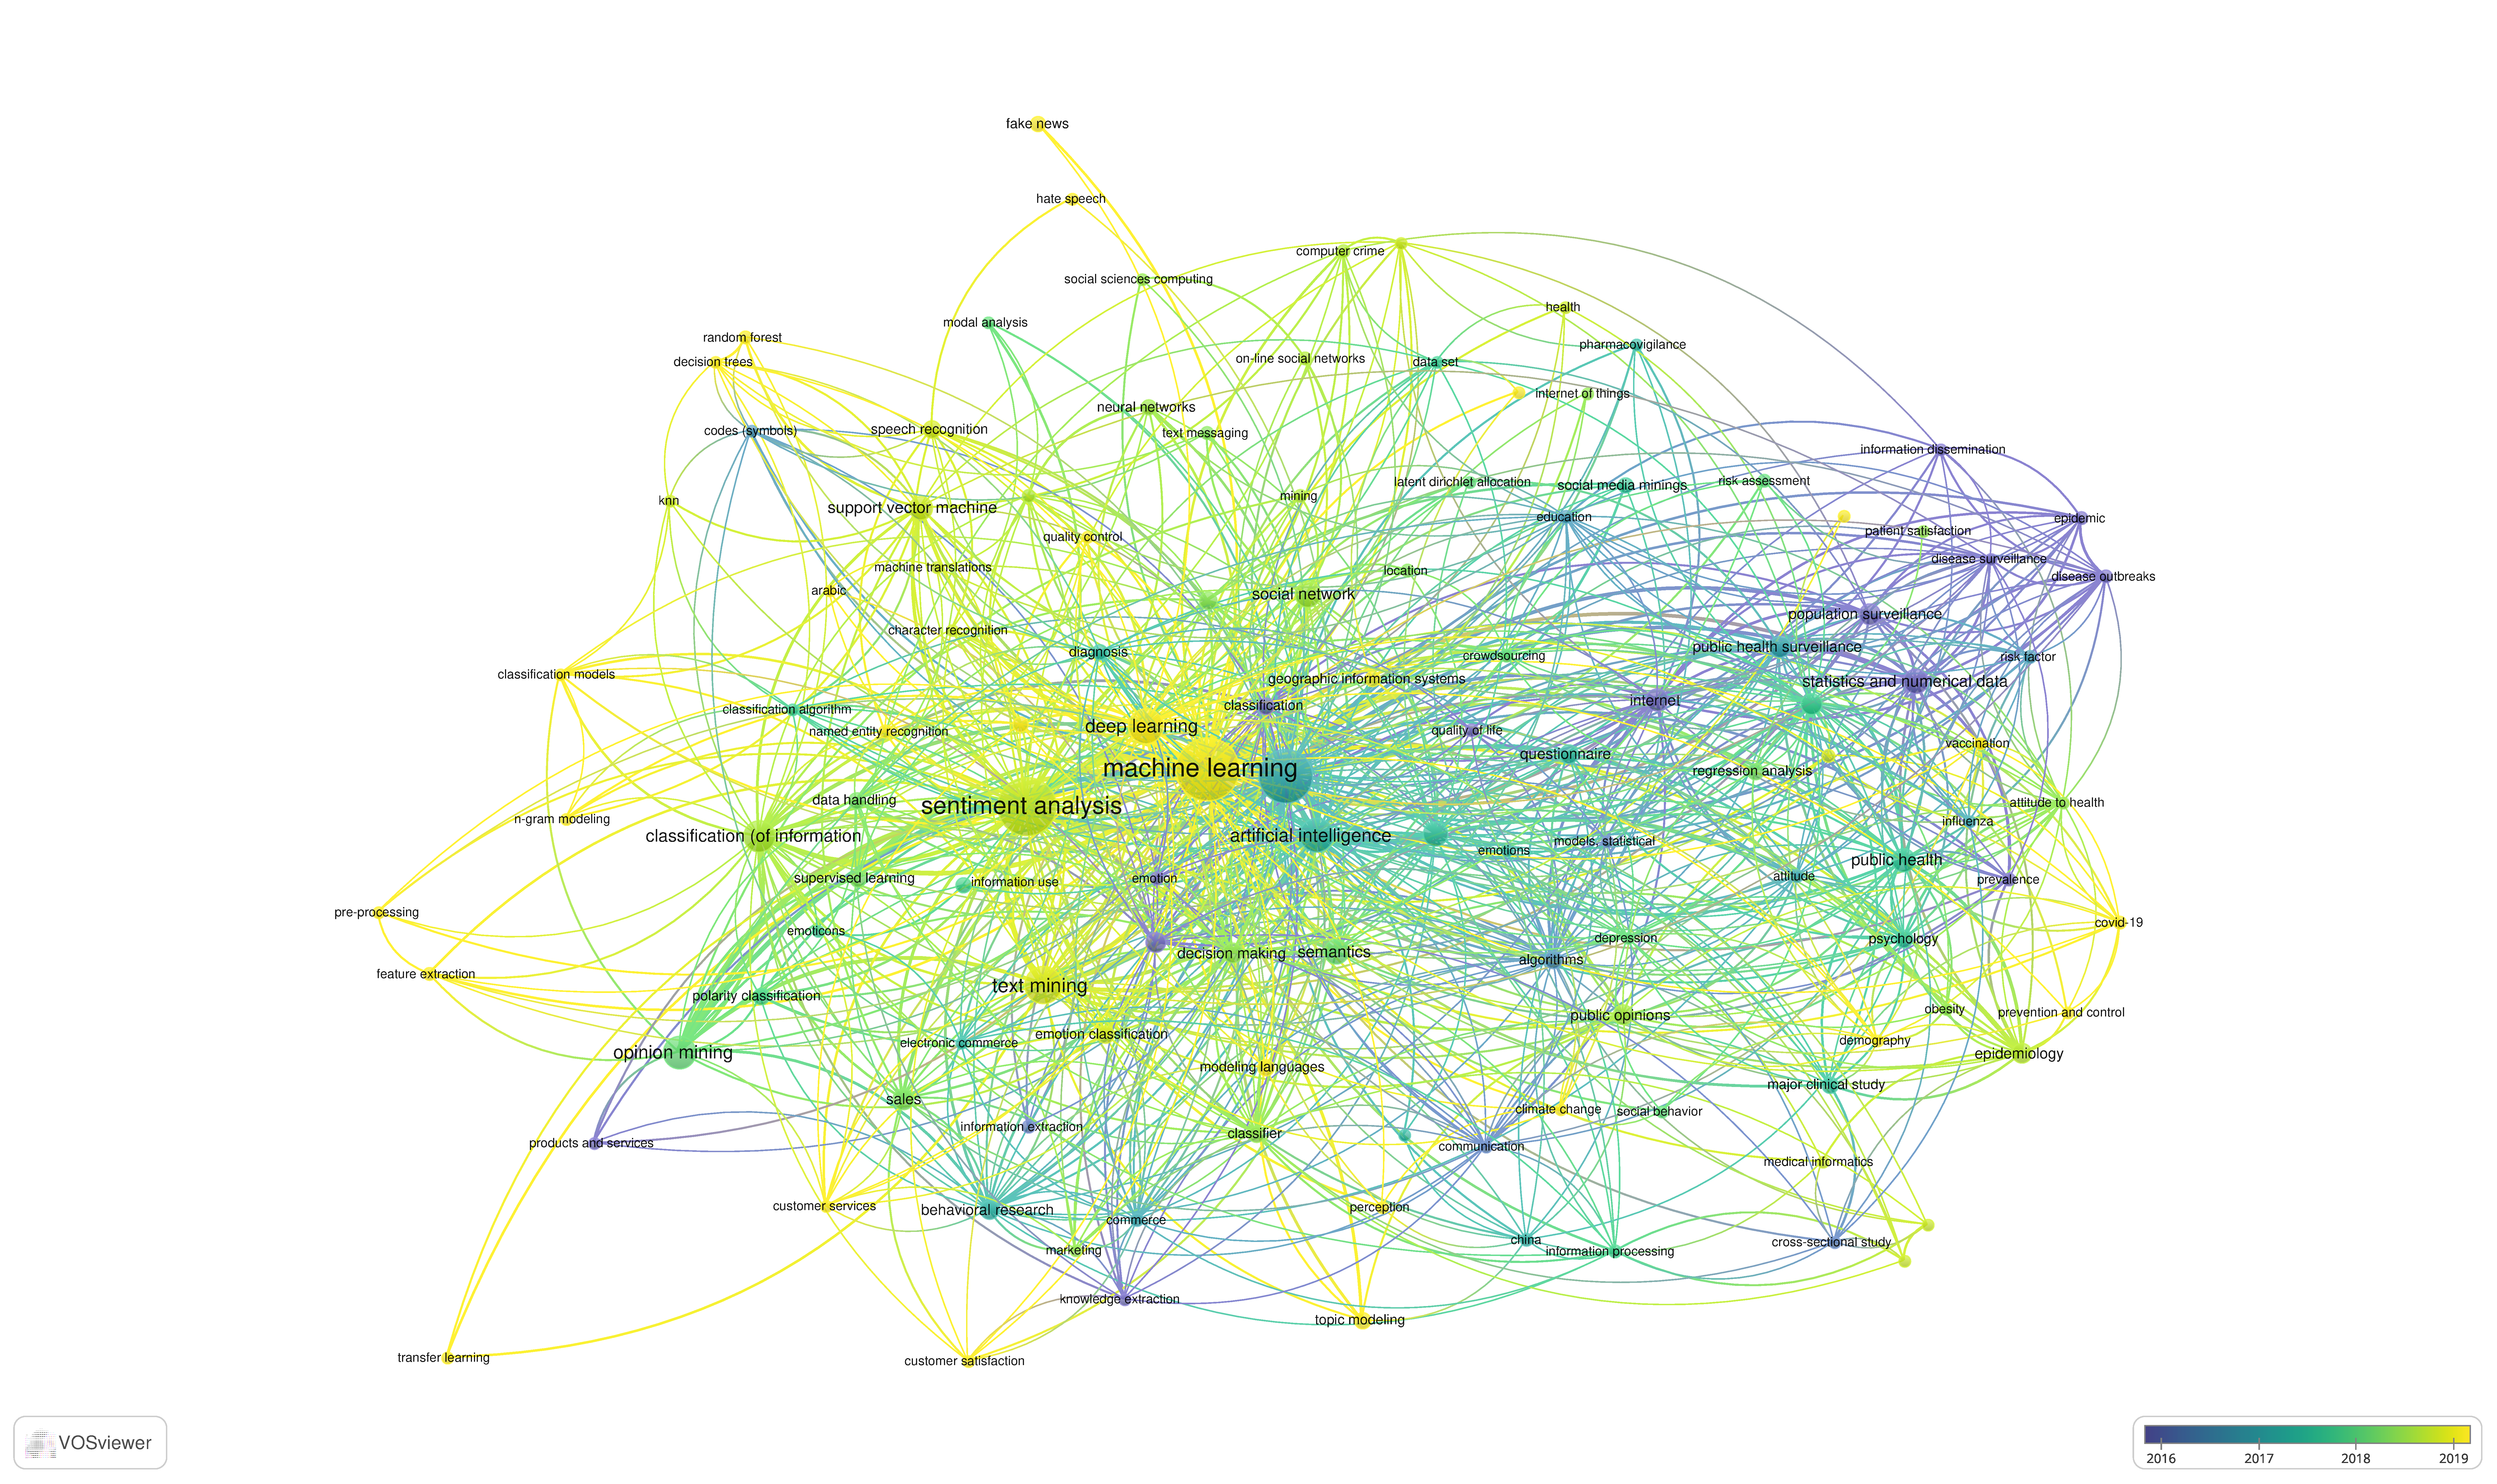
\includegraphics[width=\paperwidth,height=\paperheight,keepaspectratio, angle=90]{figures/chap-2/nlp-overlay.pdf}
    \caption{Distribution of keywords with more than 3 occurrences among the articles from the query on crisis informatics. }
    \label{literature:nlp-overlay}
\end{figure}



From the figure, it is possible to identify at least 2 clusters.
One cluster is oriented towards social and health sciences and applications of NLP on social media data in these domains.
The second one is more oriented towards computer sciences, specific algorithms and other applications domains.

Looking at the keywords that are common to at least 3 articles, we can identify several domains of application appear.
The keywords used by both the publishers and the authors also provide interesting insights.
Analyzing the keywords, three sets emerge:
\begin{itemize}
    \item Application domains: researchers identified areas of applications for NLP associated with social media data.
    \item Problem solving: general challenge of NLP translated to social media data or specific issue related to social media data.
    \item NLP techniques: the algorithms, approaches used to solve the previous challenges and relevant to an application domain.
\end{itemize}
For clarity, similar keywords (e.g. "emotions", "emotions analysis") are merged together in the tables for brevity.
The two following tables correspond to the two first sets (application domains and problem solving).
The next section dive deeper into the most common NLP techniques used.

Table~\ref{table:application-domains}

Many keywords where common to multiple topics. So instance "attitude" refers both to ...
"Quality of life" is used to urban issues, breast cancers, depression detection, opioids side effects.

\begin{center}
    \begin{longtable}{ rr }
        \hline
        Major domain          & Sub domains                     \\ [0.5ex]
        \hline
        Epidemiology          & COVID-19                        \\
                              & disease outbreaks               \\
                              & disease surveillance            \\
                              & vaccination                     \\
                              & epidemic                        \\
                              & epidemiology                    \\
                              & influenza                       \\
        \hline
        Medical Informatic    & depression                      \\
                              & diagnosis                       \\
                              & psychology                      \\
                              & public health surveillances     \\
                              & health survey                   \\
                              & risk factor                     \\
                              & major clinical study            \\
                              & medical informatics             \\
                              & obesity                         \\
                              & opiate addiction                \\
                              & opioid-related disorders        \\
                              & patient satisfaction            \\
                              & pharmacovigilance               \\
                              & pregnancy                       \\
                              & prevalence                      \\
                              & prevention and control          \\
                              & quality control                 \\
                              & risk assessment                 \\
                              & controlled study                \\
        \hline
        Behavioral Research   & social behavior                 \\
                              & models, statistical             \\
                              & social network                  \\
                              & computer crime                  \\
                              & public opinion                  \\
                              & population surveillance         \\
                              & demography                      \\
                              & smart city                      \\
                              & risk assessment                 \\
        \hline
        Social Media Research & facebook                        \\
                              & social media mining             \\
                              & fake news                       \\
                              & modal analysis                  \\
                              & data mining                     \\
                              & information dissemination       \\
                              & opinion mining                  \\
                              & perception                      \\
        \hline
        Business              & commerce                        \\
                              & customer services               \\
                              & sales                           \\
                              & communication                   \\
                              & electronic commerce             \\
                              & marketing                       \\
                              & products and services           \\
        \hline
        Information Science   & knowledge extraction            \\
                              & information systems             \\
                              & classification (of information) \\
                              & gis                             \\
                              & decision making                 \\
                              & information extraction          \\
                              & information processing          \\
        \hline
        NLP challenges        & machine translations            \\
                              & speech recognition              \\
                              & polarity classification         \\
                              & location inference              \\
                              & text mining                     \\
                              & automated detection             \\
                              & named entity recognition        \\
                              & arabic languages                \\
                              & linguistics                     \\
                              & topic modeling                  \\
                              & emotion analysis                \\
                              & sentiment analysis              \\
                              & emoticons                       \\
                              & modeling languages              \\
        \hline
        No specific category  & china                           \\
                              & education                       \\
                              & crowdsourcing                   \\
                              & climate change                  \\
                              & quality of life                 \\
                              & attitude                        \\
                              & internet of things              \\
                              & spatiotemporal analysis         \\
                              & surveys and questionnaires      \\
        \hline
        \caption{Applications domains}
        \label{table:application-domains}
    \end{longtable}
\end{center}

% Crisis informatic is not listed here – there are different definition of application domains
\cite{farzindarNaturalLanguageProcessing2017} identify several applications of NLP for social media data.
\begin{itemize}
    \item Geo-location detection
    \item Entity linking and Disambiguation
    \item Opinion mining and emotion analysis
    \item Event and topic detection
    \item Automatic summarization
    \item Machine translation
\end{itemize}

\subsection{NLP's tools to process previous data}

Along with this list of application, we can add the list of NLP techniques listed alongside:
\begin{table}[bp]
    \centering
    \begin{tabular}{rr}
        Major category          & Sub category                 \\ [0.5ex]
        \toprule
        Data management         & Big Data                     \\
                                & Pre-processing               \\
                                & N-gram Modeling              \\
        Artificial intelligence & Artificial Intelligence      \\
                                & Algorithms                   \\
                                & Classification Algorithms    \\
                                & Regression Analysis          \\
                                & Statistical Model            \\
                                & K-Nearest Neighbors          \\
        Machine learning        & Classifiers                  \\
                                & Supervised Learning          \\
                                & Feature Extraction           \\
                                & Decision Trees               \\
                                & Random Forests               \\
                                & Latent Dirichlet Allocation  \\
                                & Support Vector Machine       \\
        Deep learning           & Neural Networks              \\
                                & Classification Models        \\
                                & Transfer Learning            \\
                                & Convolutional Neural Network \\
                                & Recurrent Neural Networks    \\
        \bottomrule
    \end{tabular}
    \caption{Main NLP algorithms and techniques that appear among the keywords}
    \label{table:nlp-tools}
\end{table}

% Faire une partie qui décrit chaque point et les articles associés.
% Conclusion: le traitement des médias sociaux à très largement profité des avancées successives en intelligence artificelles qui ont été appliqués au NLP.
% Cette tendance s'observe temporellement, avec un léger décalage entre le moment ou l'algorithme/la techique devient mainstream et son adoption.

% \subsection{Processing of whole messages in social media data}
% - Informations à l'échelle du message complet (métadonnées + texte)
% - Informations à l'échelle du message textuel
% - Informations à l'échelle des mots du message.

% \begin{table}[bp]
%     \centering
%     \renewcommand{\arraystretch}{1.5}
%     \begin{tabular}{m{0.3\textwidth} m{0.7\textwidth}}
%         Reference                                             & Features \\ [0.5ex]
%         \toprule
%         \cite{liuSentimentAnalysisOpinion2012a}               &          \\
%         \cite{liuSurveyOpinionMining2012a}                    &          \\
%         \cite{collierUncoveringTextMining2012a}               &          \\
%         \cite{chamlertwatDiscoveringConsumerInsight2012a}     &          \\
%         \cite{bontchevaMakingSenseSocial2014a}                &          \\
%         \cite{vazquezClassificationUsergeneratedContent2014a} &          \\
%         \cite{raviSurveyOpinionMining2015a}                   &          \\
%         \cite{santillanaCombiningSearchSocial2015a}           &          \\
%         \cite{karmenScreeningInternetForum2015a}              &          \\
%         \cite{odlumWhatCanWe2015a}                            &          \\
%         \cite{linUncertaintyAnalysisCrowdsourced2015a}        &          \\
%         \cite{wangSocialMediaSensor2015a}                     &          \\
%         \cite{bahkPubliclyAvailableOnline2016a}               &          \\
%         \cite{paulSocialMediaMining2016a}                     &          \\
%         \cite{hawkinsMeasuringPatientperceivedQuality2016a}   &          \\
%         \cite{jiangAssessmentOnlinePublic2016a}               &          \\
%         \cite{bailCombiningNaturalLanguage2016a}              &          \\
%         \cite{kagasheEnhancingSeasonalInfluenza2017a}         &          \\
%         \cite{martinezPatientUnderstandingRisks2017a}         &          \\
%         \cite{poriaReviewAffectiveComputing2017a}             &          \\
%         \cite{yazdavarSemiSupervisedApproachMonitoring2017a}  &          \\
%         \cite{charyEpidemiologyTweetsEstimating2017a}         &          \\
%         \cite{salloumSurveyTextMining2017a}                   &          \\
%         \cite{sailunazEmotionDetectionText2018a}              &          \\
%         \cite{chaturvediDistinguishingFactsOpinions2018a}     &          \\
%         \cite{haririUncertaintyBigData2019a}                  &          \\
%         \cite{hemmatianSurveyClassificationTechniques2019a}   &          \\
%         \cite{yadavSentimentAnalysisUsing2020a}               &          \\
%         \bottomrule
%     \end{tabular}
%     \caption{Articles on informational needs of emergency responders retrieved from the previous request with at least 25 citations.}
%     \label{table:nlp-main-articles}
% \end{table}

%TODO Conclusion de la section  : qu'est-ce que finalement on peut exploiter comme information à partir des médias sociaux à l'aide du NLP

\section{Conclusions on the literature and identified gaps}
% Table with the business needs and the technical solution. Align both of them.
This section conclude the literature review and its outcome.
It takes the form of a table with two entries.
The first one is the identified informational needs of the decision makers.
The second one is the different technical solutions explored to extract information from social media data.
The contribution of this manuscript hold in the gap between these two domains.

1. Pas ou peu d'analyse du besoin des personnes qui utilisent les médias sociaux en situation de crise. Des classifications à l'arrache, parce qu'elle me plaît, parce que j'ai envie, parce que mon voisin à dit c'est cool.
-> Un modèle de situation de crise pour qui ? Pour quoi ?
2. Des tonnes d'architectures différentes, en fonction de comment le graduate a souhaité l'implémenter. Pas/peu de solution pour implémenter des données.
-> MLOps appliquées à notre problématique + mon architecture HICSS
3. Beaucoup de travaux pour classifier des messages. Peu de travaux sur le traitement à l'échelle du mot.


%%% Local Variables:
%%% mode: latex
%%% TeX-master: "../ma-these"
%%% End:


\chapter{Crisis situation models that serve social media operators}


\section*{Introduction}
% Jonction entre le : "quel modele je peux constuire avec les donnees issues de medias sociaux" et "de quoi on besoin les gens qui utilisent les media sociaux en gestion de crise" %%
Reference to chap. 1 and chap.2 to emphasized on the collaboration.
Collaboration happens during all the phases of the crisis management cycle.
However the focus will be on the response phase.

Coordination of the response requires collaboration.
Collaboration requires information sharing.
Yet, information sharing is problematic as actors need a common vocabulary to talk about things that everybody can understand.
Also, these information need to be served in a common way to all the actors (come back to the COP).
These measures facilitate the decision making of all the actors.
Finally, decisions made by each actors need to be passed to the other actors.

What are the information that people looking at social media need to share with decison makers?
Thus, this chapter focuses on two aspects:
\begin{itemize}
    \item Who look at social media and what are they looking for?
    \item Which information model is it possible to build using social media data?
\end{itemize}

\section{Who process social media during crisis response?}
Crisis management involve multiple actors (see chap. 1).
Thus, not all member of the organization are dealing with social media processing.
This section aims at clarifing the first part of the original problematic: who are the person dedicated to social media content processing during emergency events?

The argumentation in this section is mostly anecdotical, with the meetings with the US 911 and MACIV exercices.
The MACIV project was really insightful in this regard.
Multiple occasions to witness the organization of crisis management, while it wasn't the exact focus of the project (mostly information focused).

For the US: call centers (handling it as the regular calls, with people checking social media for information).
The information is then sent to the dispatchers or to the crisis cell if there is one.
In France: a third party watch social media (VISOV association) and their results are then consolidated in the emergency management centers upon request

Conclusion: Here are the different profils identified that are facing social media during an emergency event.
2 things: they use it to obtain information from social media for 2 purposes:
\begin{itemize}
    \item Help organize the response on the field (information consolidation)
    \item Orient their communication to the public (information dissemination)
\end{itemize}
Also, important to mention that from my perspective, the population of call centers/emergency centers that are interesed in social media is not the majority of them.
So there is room for improvement here.

\section{Information needs identified}
Qu'est-ce que les profils cherchent concrètement lorsqu'ils regardent les médiaux sociaux ?

- Partie terrain (Jess - 6W)
- Partie "+ remote" (Audrey - Robin ...)

\subsection{Situation awareness}
- Situation awareness according to Endsley
- Situationa awareness adapted to NLP for crisis response

\subsection{Actionable information}
- Jess Kropczynksi's interviews. 6W's
- Zahra's survey and interviews
- Others?

=> Voici les informations dont ils ont besoin (definitions SA et AInf ici?)

\section{Intersection with crisis situation models}
- Intersection with the high level crisis situation models presented in the LR and the "feedbacks from the field".
- My article ISCRAM 2021 (for the need to ackownelge the users' needs in the design of social media processing systems) and HICSS 2021 (for the classification of information that we are looking at).

Retour sur les models d'information pour le CM.
1. Filtrer les modeles qui n'incluent les utilisateurs precedement identifies dans leurs scopes
2. Identifier les classes utilises par ses modeles qui representent l'information dont les utilisateurs ont besoin

=> Classes that are relevant for the end users/classes we will search for.

\section{Conclusion}
- We figured what information we were looking for. Now, how do we extract those information? How do we implement the associated classes of the metamodel?
- Update the table in the LR with the identified needs

=> Voila le model des informations qu'on peut esperer pour la crise pour les personnes en des medias sociaux

Next chapter deals with the ways to extract the information identified in this chapter.

\section{Who process social media during crisis response?}
\begin{itemize}
    \item 911 calls takers, social media experts in the US (meetings with the operators of the call centers)
    \item Social media operators in France (MACIV exercices)
\end{itemize}

\section{Needs identified}
\subsection{Situation awareness}
\begin{itemize}
    \item Situation awareness according to Endsley
    \item Situationa awareness adapted to NLP for crisis response
\end{itemize}

\subsection{Actionable information}
\begin{itemize}
    \item Jess Kropczynksi's interviews. 6W's
    \item Zahra's survey and interviews
    \item Others?
\end{itemize}

\section{Intersection with crisis situation models}
Intersection with the high level crisis situation models presented in the LR and the "feedbacks from the field".
My article ISCRAM 2021 (for the need to ackownelge the users' needs in the design of social media processing systems) and HICSS 2021 (for the classification of information that we are looking at).

=> Classes that are relevant for the end users/classes we will search for.

\subsection{Conclusion}
We figured what information we were looking for. Now, how do we extract those information? How do we implement the associated classes of the metamodel?
Update the table in the LR with the identified needs


%%% Local Variables:
%%% mode: latex
%%% TeX-master: "../ma-these.tex"
%%% End:


\chapter {Identification of relevant entities in social media data for crisis response: a semi-supervised approach}

\section*{Introduction}
The first chapter presented the need to gather and organize information at the time of crisis
response.
At the very onset of the event, information is lacking, and therefore,
impedes the coordination and proper dispatching of needed actors and resources.
The literature review highlighted that; meanwhile, crisis management organizations have
voiced their need for tools to process the high volume of data produced by social media
and share the information obtained with other actors of the response.
The previous chapter, Chapter 3, assessed the information that decision-makers expect.
This statement is the motivation behind the second research question: \textit{How can the actionable information available on social be automatically retrieved during crisis response?}
Similarly, the positioning of this chapter with respect to the body of this dissertation is illustrated Figure~\ref{processing:big-picture-manuscrit}

\begin{figure}[htb]
    \centering
    \includegraphics[width=\textwidth]{figures/chap-4/position-chapter.pdf}
    \caption{Location of this chapter in relation to the body of this manuscript.}
    \label{processing:big-picture-manuscrit}
\end{figure}

This chapter presents a new approach to processing social media data to support automatically
the operators in charge of information recovery during disaster response.
This approach aims to gather the information required by decision-makers in the context
of disaster response, i.e., information that fits within the information model presented
at the end of the previous chapter (Figure~\ref{information:information-models}).

This approach is based on machine learning and seeks to identify the information expected
by decision-makers within the messages posted on social media.
Unlike most of the other approaches that process the social media information in this context, the processing is not performed at the scale of the message itself.
Instead, the message is processed at the scale of the different terms that compose the message.
The method relies on previous work realized on this topic to take the processing of the data a step further.
Figure\ref{processing:social-media-processing} illustrates the positioning of our contribution in the light of previous work.
The objective is to facilitate the processing, and thus to save time, on data processing.

\begin{figure}[htb]
    \centering
    \includegraphics[width=\textwidth]{figures/chap-4/social-media-processing.pdf}
    \caption{Positioning of our contribution with respect to other social media processing tools.}
    \label{processing:social-media-processing}
\end{figure}

The chapter describes in a first section the context of the problem and the constraints
that motivated the design choices for the model.
The second section describes the model and explains the methodology used behind the development.
The last section is devoted to evaluating the model's performance and to the
discussion of the latter in the context of crisis management.

\section{Problem diagnosis}
The previous chapter highlighted the needs encountered by crisis management actors at the
response time.
Specifically, they call for better ways to retrieve their situational awareness and strengthen it, to improve their decision-making.
Among the proposed solutions, we find the idea of sharing actionable information through
a cartographic representation: the Common Operational Picture.
The Common Operational Picture is fed by the information available to each actor, which is then transmitted to
all actors through a common vocabulary or concepts shared by all actors.

However, as also identified in the previous chapter, information retrieval is not performed
by the decision-makers themselves.
Dedicated operators are charged with information retrieval on different information channels
(reports, calls made to the call centers, news, social media, etc.).
The call takers have thus developed frameworks that allow them to obtain information
aligned with the needs of the decision-makers.
Social media, however, due to the high volume of data and the noise/information ratio,
raise new challenges.
The literature review in Chapter 2 highlighted the trend toward automation in crisis informatics.
This trend is intended to reduce the monitoring burden that operators must bear to achieve their results.
In addition, crisis response is usually not an environment that leaves room for insufficiently
effective resources.

The objective is, therefore, to bring together two aspects: (i) processing of social media
that corresponds to the information needs of the decision-makers and
(ii) support in the handling of the volume of data that social media operators are facing.

\subsection{Core problematic}
Social media make available a significant volume of data in the form of text, photos, or videos.
Processing social media content is tedious and harder when compared directly with phone calls.
This is due to the fact that most of the data are unrelated to the current event operators are interested in.
Therefore, they are looking for tools that could help them in their task.

The crisis informatic domain takes on the challenge to provide useful tools that would help in processing social media data.
To reduce the load of the operators, many approaches have been taken.
The first approach consists in increasing the processing capacity through the help of volunteers.
Crowdsourcing tools allow the former to help in the classification of the messages that can then be forwarded to decision-makers \parencite{imranAIDRArtificialIntelligence2014}.
A second approach is to lower the incoming flow of data that the operators are facing.
Some explored ways to reduce the noise part of the flow by filtering messages according to their relevance (linked or not to the ongoing event) \parencite{carageaClassifyingTextMessages2011,imranAIDRArtificialIntelligence2014}.
Others attempted to shrink the incoming flow as a whole by summarizing the information from the incoming data \parencite{rudraSummarizingSituationalTweets2016}.

Emergency responders encounter several problems when they have to process social media.
(i) there is a high volume of data, and (ii) they have to screen each individual message
to extract information, regardless of its interest.

Thus, the solution proposed has to cover two aspects:
\begin{itemize}
    \item It has to reduce the time spent in the processing of incoming messages by reducing the number of unrelated messages and the time spent screening the text to identify relevant information in the flow.
    \item It has to deliver value to the decision-makers by providing the information required by the different actors. The information retrieved should consequently match the concepts used in the Common Operational Picture.
\end{itemize}

The approach presented in this chapter aims to address both aspects.
The contribution builds on previous work that largely addressed the first aspect in
order to address the second part of the problem, which remains essentially unexplored.
The solution proposed in this chapter, and developed in the next parts, highlights the useful entities for decision-makers in the incoming messages.
Therefore, the goal is to highlight in the messages the information that corresponds to
the concepts presented at the end of Chapter 2.

\subsection{Machine learning in disaster response context}
As highlighted in the second chapter, many advances have been realized using machine learning approaches.
These advances greatly benefited natural language processing and provided tools to tackle
new challenges.
However, after time spent with crisis management professionals, one may wonder if
state-of-the-art machine learning models are really suited to the context of crisis response.
There are three inherent aspects of machine learning that one must consider:

\begin{itemize}
    \item The "black box" aspect
    \item The data aspect
    \item The economic aspect
\end{itemize}

Machine learning is, therefore, a toolbox where each tool provides a different way of capturing patterns inherent in data and binding them to the information desired.
An underlying assumption of machine learning is that the patterns present in the data will be repeated in the future.
However, as presented in the first chapter, disasters are by nature unpredictable and are generally similar to a leap into the unknown.
In this context, there is a high degree of uncertainty about the performance of a model trained on data obtained from past disasters.
In the case of a fully unexpected crisis, a system that relies on machine learning can be rendered useless (the returned results are outliers).
The worst-case would be that the system provides erroneous results and that these results are still taken into account by the decision-makers, unaware of the errors.
These aspects are highlighted and discussed by \textcite{endsleyDesigningSituationAwareness2016} and taken up in Chapter 5.
To avoid this scenario, the author recommends including the operators in the functioning of the algorithm by allowing them to influence the results of the algorithm in the most intuitive way possible.

Machine learning approaches consume data to deliver results.
These data can be either labeled or unlabeled.
There exist different algorithms in the machine learning toolbox according to either the
data are labeled or not and correspond to a "learning mode."
The learning is said supervised when the algorithm learn under the supervision of label
example.
It is self-supervised when the algorithm uses raw, unlabeled data to extract knowledge.
An algorithm is said semi-supervised when it uses both labeled and unlabeled data to learn.
All cases require data that need to be gathered.
Labeled data requires the additional data labeling effort.
Self-supervised learning is a specific mode of learning, as it is used to generate language
models, i.e., large vectors that represent the semantic commonly associated with the syllables
found in a language.
The interest and challenges of language models are further developed later in this chapter.
In crisis informatics, most of the approaches use a supervised approach.
The community then gathered datasets of data gathered during several events \parencite{olteanuCrisisLexLexiconCollecting2014,olteanuWhatExpectWhen2015}.
However, these datasets are mostly labeled at the scale of the message itself.
Any work on a different scale, therefore logically requires additional labeling work.
This echoes the generalization problem mentioned earlier, as it is complicated to guarantee
that all the data collected will be representative of the events.
Moreover, any task that would seek to solve a problem occurring at a different scale,
such as labeling the entities present within a sentence, for example, requires a relabeling
of the data.

State of the art machine learning models may require dedicated hardware, especially the
larger models released
Very general machine learning models require adequate hardware and, therefore, a significant investment.
Consequently, running such a model is costly.
The early adopters met during the Early adopter's summit at Charleston in 2020 raised concerns
about the cost of Next-Generation 911.
State of the art machine learning models can require a significant amount of computing
resources.
This is an important consideration when developing a solution to support emergency management centers.
Machine learning is probably the most appropriate tool to solve the identified problem,
but it is important to remember that this tool is not a free lunch.

To summarize, the aim is to facilitate the processing of social media data by highlighting
the information that decision-makers need, i.e., information that is in the information
the model presented at the end of Chapter 2.
Machine learning approaches are indicated to answer this type of challenge.
However, due to the context of disaster response, one has to keep in mind that the solution
i) cannot be a black box to the end-user, ii) has to be generalist enough to be useful in
various situations, and iii) can be run in an emergency center.
A common solution nowadays to the two former constraints is to fine-tune a pre-trained
language model.
This approach associates a good ratio of performance/data labeled and are requiring reasonable
hardware to run.
However, this approach always requires a significant amount of labeled data, representative
of the data that the model will process in the future.
This approach has already been used to classify the relevance of messages posted on social media \parencite{kozlowskiThreelevelClassificationFrench2020}.
However, it is not exactly suited to the context previously described as it does not:

\begin{itemize}
    \item The model act as a black box, as the end-user cannot interact with its results.
    \item There is no labeled data suited for the task
    \item The results provided in case of unseen events are hard to predict.
\end{itemize}

The next sections present a solution that addresses the initial research question while taking
into account the previous limitations.
The first section focuses on the training phase and the second section presents the use
of the method and its performance on an evaluation set.

\section{Scientific foundations of the approach}
The previous problem is similar to a named entity recognition problem.
It seeks to i) locate and ii) label the named entities (brand, person, organization, location etc.) contained in a sentence.
However, instead of looking for named entities, our approach aims to identify predefined
entities, which in our case are the different concepts of the information model.
The proposal is to train a machine learning model in a semi-supervised way able to recognize the entities that belong to the different classes.
The approach relies on two properties of the most recent language models.
First, they allow to "translate" textual data into vectors.
In our case, each word, labeled or not, is associated with a vector.
Secondly, the word vector is obtained from a vector space, whose distance between the different
vectors represents the semantic similarity between the words.
This vector space thus contains clusters of vectors composed of semantically similar entities.
These vectors are obtained by processing the data of the vector space with a clustering algorithm.
It is from this step that the labeled data intervene in the method.
The terms labeled by the operators are included with the other terms.
Therefore, they appear in some of the clusters identified previously.
The labeled terms are used to associate the non-labeled content of the clusters with the labels.
The labels are then propagated from the labeled terms present in a cluster to the non-labeled terms.
In this way, the non-labeled terms semantically close to the labeled terms are associated with the different concepts we are trying to identify.
The different steps of the algorithm are outlined in Figure~\ref{processing:big-picture}.
The method is composed of four main steps after data normalization.
These are:

\begin{enumerate}
    \item Generation of the word vectors associated with each token.
    \item Dimension reduction of the vector space obtained previously to facilitate the following clustering.
    \item Identification of semantic clusters present in the vector space using a clustering algorithm.
    \item Label propagation within the different semantic clusters.
\end{enumerate}

The next sections detail and present the choices that led to the different elements represented.

\begin{figure}[htb]
    \centering
    \includegraphics[width=\textwidth]{figures/chap-4/big-picture.pdf}
    \caption{Overview of the approach developped in this chapter.}
    \label{processing:big-picture}
\end{figure}

The semi-supervised approach implies that the training is made using two distinct datasets.
One dataset contains labeled data, and the other contains unlabeled data.
The former, in our approach, contains text messages obtained from previous disaster events.
These messages are sliced to obtain a list composed of the entities that make up the message.
The term "entity" is used here to reflect the fact that, on social media, the message can be composed of other elements than words, like URLs for example.
This process of breaking down sentences is called text tokenization.
Unlabeled sentences are thus broken down into lists of corresponding tokens.
Once all messages are split, a vocabulary is created.
This vocabulary is composed of all the unique entities that are used in the original text messages.
The labeled dataset is composed of words/tokens that are paired with one of the labels of the information.
The two sets of tokens are then merged to create a set of unique tokens, where some are labeled.
The next section presents how language models convert these tokens to vectors that embed the semantic of each token.

\subsection{Language models and semantic representation of textual data}
Texts can be seen as data with two components: a syntactic one and a semantic one.
The syntax composes the form of the text, the graph of the words, and how they combine to create the sentences.
The semantic compose the meaning of the text, the ideas that the text has to convey through a statement.
Computers have many means to process the syntactic part of textual data but lack tools to process the meaning of character strings.
The Natural Langage Processing domain developed different approaches and tools to represent the semantic part of data.
Language models are one of these tools.
They are statistic models that represent the probability distribution over sequences of symbols used to create sentences.
These symbols can be words, letters, or phonemes.
The probability distribution is built assuming that languages have a distributional structure \parencite{harrisDistributionalStructure1954}.
This assumption states that the meaning of a word in a given sentence is provided by the words surrounding it.
The same reasoning is applied at the different scales of symbols mentioned earlier.
Most recent languages models rely on neural networks to construct the probability distribution.
The neural network is trained to predict the probability distribution of words in the different sentences used as training examples.
Instead of producing the probabilities distribution, the distributed representation encoded
in the networks' "hidden" layers are used to represent each word.
Each word is then mapped onto an \(n\)-dimensional vector of reals called a \textit{word embedding}.
Here, \(n\) is the size of the last hidden layer, just before the output layer.
The representations obtained have the distinct characteristic that they model
semantic relations between words as linear combinations.

This approach was popularized with the Word2Vec model proposed by \textcite{mikolovDistributedRepresentationsWords2013}.
Improvements to this method were conducted with models such as GloVe and FastText \parencite{bojanowskiEnrichingWordVectors2016,penningtonGloveGlobalVectors2014}.
Consecutively, attention-based models, able to embed the semantic in longer sentences, appeared.
This new generation of self-trained models is led by architectures such as ELMo, BERT, or GPT \parencite{devlinBERTPretrainingDeep2018,petersDeepContextualizedWord2018}.
Following a similar trend as with Word2Vec, improvements were conducted on this model to increase its performance.
The main differences with this new generation of models are their size (up to hundreds of billions) and their training process.
As explained in the RoBERTa article \parencite{liuRoBERTaRobustlyOptimized2019}, their size makes the training process challenging as they require significantly more training data with a wider variety.
Languages models have also been trained using data specific to a problem, using previously mentioned architectures.
The crisis informatic domain attempted to create crisis-specific BERT models \parencite{liuCrisisBERTRobustTransformer2021}.
However, these models are usually limited by the small amount of data available, in comparison to the volume of data generally used to train this type of model, and this despite the best
collection efforts of the community.
Also, these models are not necessarily made available to the research community, like in the previous reference case, which impedes progress as they are very costly to train.
This approach produces more compact representations, compared to previous methods, whose dimension grows proportionally to the number of unique words contained in the training dataset.
Embedding layers create an arbitrary-sized vector of each word that incorporates semantic relationships.

The proposed method relies on the word embedding of a language model.
The word embeddings are used to produce vectors associated with each token of the set previously created.
These vectors then create a vector space, where the distance between two vectors is equivalent to the semantic similarity between the two vectors.
This property creates a vector space where some vectors, representing semantically close tokens, are spatially close too (see step 1 in Figure~\ref{processing:big-picture}).
The next step is then to identify these "semantic clusters" in the vector space.
This will then allow linking the unlabeled tokens of a cluster to the labeled tokens that are part of the same cluster.
This is achieved by using a label propagation approach within the clusters.
However, while the resulting vector spaces are called "low-dimensional," their dimensions are still too important for clustering algorithms to identify relevant clusters.
Consequently, their dimension is first reduced.
The next section presents the motivation and the algorithm used to perform the dimension reduction.

\subsection{Dimension reduction: UMAP}
The main objective of reducing the dimensionality of a vector space is to avoid facing the
so-called "curse of dimensionality" \parencite{bellmanDynamicProgramming1966}.
This "curse" refers to counterintuitive phenomena that appear in high-dimensional spaces.
For instance, as the dimensionality increases, the volume space increases exponentially.
Thus, data become too sparse, and the notion of distance becomes obsolete.
Dimension reduction is then often used to provide visualizations of high-dimensional spaces.
It consists in transforming data from their original space, to a space of lower dimension.
As this projection necessarily results in information loss, the goal is to find the transformation
that will keep most of the meaningful information.
There are two means (that are often combined) of achieving the projection:
(1) the extraction of the meaningful components and
(2) the projection of the data to a lower-dimensional space.
In practice, most of the algorithms developed to use both approaches.
They first identify or extract meaningful components or representations of the data and then project these to a lower-dimensional space in a way that will preserve most of the original structure of the data.
Among all the available methods and algorithms, the Principal Components Analysis (PCA) is very prominent \parencite{hotellingAnalysisComplexStatistical1933}.
This linear method creates a mapping between the original high-dimensional space and the low-dimensional destination space to ensure minimal loss of information.
The output of the algorithm consists of the vectors used for the linear mapping.
This result is explainable, hence explaining the wide adoption of this method partially.
However, this method shows limitations as the number of dimensions increase.
Indeed, the assumption of the linear distribution of the data becomes less and less correct as of the number of dimensions increases.
As a result, non-linear alternatives have been developed.
Most of these approaches rely on kernels or intermediate representations.
Recently, new approaches based on optimization methods gained significant traction thanks to their ability to provide visualizations that capture the original vector space's global and/or local properties.
For instance, t-distributed Stochastic Neighbor Embedding (t-SNE) uses a low-dimensional
map using probability distributions of data points \parencite{maatenVisualizingDataUsing2008}.
However, t-SNE is only currently capable of reducing to a two or three-dimensional space.
Uniform Manifold Approximation and Projection for Dimension Reduction (UMAP) uses a fuzzy
topological structure to represent the data structure \parencite{mcinnesUMAPUniformManifold2020}.

UMAP can be simplified as a two-step process.
The first one consists of building a weighted topological graph representing the latent structure formed by the vectors in the space of the initial dimension.
The particularity of this graph is that edge weights are not fixed values, but probabilities
that represent the distance instead.
The second step is to transpose the fuzzy weighted graph into the lower-dimensional space.
For this, UMAP builds a new graph in the arrival space in the same way as in the first step.
Creating the best graph in the target space corresponds to an optimization problem where the objective is to find the low dimensional representation with the closest fuzzy topological structure.
Given the setup of the problem, where edges of both graphs are represented using probability distributions, the goal is to minimize the cross-entropy between both probability distributions.
The cross entropy formula takes in two probabilities distributions \(p(x)\) and \(q(x)\),
defined over the discrete variable \(x\), with \( p \in \left\{y,1-y\right\}\) and \( q \in \left\{\hat{y},1-\hat{y}\right\}\)
where \(y\) is the set of input probabilities and \(\hat{y}\) the set of output probabilities.
The formula is given by
\[H(p,q)=-\sum_{\forall x}^{} p\left(x\right) log\left(q\left(x\right) \right)\ = -y log\left(\hat{y}\right) - \left(1-y\right) log\left(1 - \hat{y}\right)\]

Cross entropy allows scoring the difference between the original graph
constructed from the high dimensional data and the constructed arrival graph.
\(p(x)\) is referred to as the true distribution and is represented by the edges obtained from
the original graph.
\(q(x)\) is the distribution of the edges of the arrival graph.
The probabilities of the edges of the arrival graphs are optimized using a Stochastic
Gradient Descent process, which uses the cross-entropy as loss function.

Four main parameters then drive the algorithm:

\begin{itemize}
    \item Number of neighbors: intervenes in the construction of the weighted topological graph and balances the role of the local versus the global structure of the data in the end result.
    \item Minimum distance: represents the minimum distance the algorithm can use between several points (assists in forming dense clusters if needed).
    \item Number of components: the dimensionality of the reduced dimension space in which the data will be embedded.
    \item Distance metric: the distance metric used by the algorithm.
\end{itemize}

The dimension reduction is associated with a compromise left to the user of the algorithm.
Indeed, reducing the dimension of the vectors too much can lead to a significant loss of information.
This compromise also depends on how the reduced dimension space is used.
In our case, it is the grouping of the data into clusters supposed to represent sets of words with similar semantics.
The following section presents, in the same way as for UMAP, HDBSCAN, the algorithm chosen for clustering.

\subsection{Clustering: HDBSCAN}
Clustering consists of grouping sets of data that share similar properties.
This similarity is then represented as the distance between data points.
The representation of data in the form of vectors determines the similarity between data more obvious.
This similarity, or distance, can then be computed as the vector product (or L2 distance) or the cosine between these two vectors.
Many algorithms create clusters of data using different distances.
These algorithms are grouped according to the approach they use to create the clusters.
They can be grouped as below:

\begin{itemize}
    \item the hierarchy (decision tree)
    \item the center of gravity (K-Means)
    \item the distribution of the data (Gaussian mixtures)
    \item the density of the data (DBSCAN/OPTICS)
\end{itemize}

Each approach has its strengths and weaknesses.
Depending on the problem and the objective we want to reach, we will choose one approach.
For example, algorithms based on the centers of gravity often require the number of clusters to be identified.
This assumption is restrictive, primarily when the number of clusters searched is not known a priori.
Thus, other approaches have been developed for the discovery of clusters without a priori knowledge of the number of clusters.
These approaches focus more on the density or distribution of the data to declare the presence of clusters.
Another advantage of this approach is identifying data points that do not belong to any cluster.
In the context of this chapter, clustering is used to identify clusters of tokens that
are close semantically in the vector space created during the previous steps.
The algorithm chosen to perform the clustering on the vector space is Hierarchical DBSCAN (HDBSCAN).
This algorithm is a variant of the DBSCAN algorithm.
The choice of HDBSCAN is made because it is a fast and not greedy clustering algorithm that allows predicting clusters for new points.

HDBSCAN extends DBSCAN with a hierarchical clustering approach where the flat clustering is extracted based on the stability of the clusters.

HDBSCAN works through 5 consecutive steps.
First, it transforms the vector space according to the density of data points.
The core is based on single linkage clustering, which is very sensitive to noise.
The impact of noise is reduced by making sure that noise data points are more distant than those belonging to a cluster.
This is achieved by using the \textit{mutual reachablity distance} between different points
that is given by
\[d_mreach-k (a,b) = \max \left\{core_k (a),core_k (b),d(a,b)\right\}\]
where \(core_k(a)\) is the distance between a point \(a\) and its farthest neighbor among
its \(k\) neighbors.

The mutual reachability distance between the data points is used to generate a graph that connects all the vertices together and with the minimum possible total edge weight.
This graph can be obtained by computing the minimum spanning tree of the graph.
Each data point represents a vertex, and the mutual reachability distance weighs the relationships between the different points.

The minimum spanning tree is used to compute the hierarchy between the clusters.
The edges of the tree are sorted by distance and iterate through each vertex to merge them to a cluster.
These three steps compose the DBSCAN algorithm.
However, the resulting clusters can only be obtained at that stage by setting a threshold at which clusters are defined.
This threshold is a parameter set by the user in DBSCAN that has to define where to "cut" the hierarchy.
This parameter is hard to set in the current situation, as the mutual reachability distance is linked to the density of the cluster.
A better approach is to cut the hierarchy tree at various places to reflect the density difference between the clusters.

The hierarchy tree is then condensed.
Instead of aggregating the data points to form clusters, the problem is turned upside down: we start with a single set that is "losing points" at each split.
To define is points are "lost", the user set a \textit{minimum cluster size}.
If a cluster has fewer points at a split than the minimum cluster size set, then the part with fewer points is dropped off the group, and the part with more points than the minimum is aggregated with the original cluster.
Conversely, if both parts have more points than the minimum cluster size at a split, then two independent clusters are created.
Using this approach, the cluster tree is much smaller than previously.
Using this condensed representation, it is now easier to extract clusters as fewer nodes and splits are in the hierarchy tree.

Just as UMAP, HDBSCAN has a lot of parameters to tune the different parts of the algorithm.
As mentioned earlier, the minimum cluster size is the main and mandatory parameter of the method.
Another parameter of interest is the number of minimum samples.
This parameter intervenes in the creation of the first hierarchy tree and influences the conservativeness of the clustering.
Large values of this parameter lead to more points labeled as noise.
It is tied with the minimum cluster size parameter and takes its value as default.
Other parameters specific to our use case are described in the experimental sections.

HDBSCAN allows identifying clusters formed by semantically close words.
The advantage of this algorithm is that it is very efficient in terms of computation and allows to distinguish efficiently points that are part of a cluster or belong to noise.
Among all the clusters thus formed, some contain some of the words initially labeled by the operator.
The next step is to propagate the labels within these clusters in an ordered way to discover new terms associated with the concepts of the information model.

\subsection{Label propagation algorithm}
The clustering algorithm has identified clusters within the data, which represent semantic clusters whose words have a joint semantic base.
However, there is no way to know to which type of information,i.e., to which label, the different clusters refer.
For this purpose, the words labeled by the operator are used.
As some of these words are located within clusters, they will be used as tags within the cluster, and their associated labels will be propagated to the rest of the cluster.
In this way, it is possible to capture many words that refer to the same concept from a few labeled terms.
Hence, a label propagation approach is used.
This method composes the core of the semi-supervision aspect of our approach.

Label propagation is a method originally designed for graphs \parencite{zhuLearningLabeledUnlabeled2002}.
For a given graph, the idea is to provide a label to some nodes of the graph and to propagate the labels of these nodes until the graph is fully labeled.
The label propagation used here, while following the same logic, is different.
The original method is actually overly aggressive in labeling the data in our setup, where the data are very similar.
To remedy this problem, some improvements have been made.

Propagation takes place within clusters that have at least one label.
Thus, there are two cases:
\begin{enumerate}
    \item There is only one label in the cluster: in this case, the label is simply propagated to all the other tokens in the cluster
    \item Several labels coexist within the cluster.
\end{enumerate}

In the former case, it needs to be controlled.
Indeed, a label should not be propagated on tokens belonging to other labels.
In the same way that we split our starting space into semantic clusters, these same semantic clusters can be split again to identify sub-clusters (referred to as "domains") of different labels.
Once the domains within a semantic cluster are identified, the label propagation is performed similarly to the case where the cluster contains a single label.
This step returns to the case where the cluster is composed of a single label.
This approach mirrors the operation of a K-Means algorithm, which slices a data space into k zones to identify clusters.
The most important parameter of this algorithm is \(k\), the number of clusters present in the data space.
However, the number of domains in a given semantic cluster is unknown at that point.
Therefore, HDBSCAN is reapplied to identify the number of domains in the semantic cluster.
The value of the parameter \(k\) used for the K-Means depends on the number of clusters identified.
Again, there are two cases here: i) there are more labels than domains identified, or ii) there are more (or the same number of) domains identified than labels present in the cluster.
In the former case, the number of domains is passed to the number as \(k\).
The K-Means will then split the space into k partitions which will become our domains.
For each domain that contains a labeled token, the label is propagated to all tokens that are part of this domain.
In the case where the number of labels is equal to or less than the number of identified domains, k takes as value the number of labeled tokens in the semantic cluster.
Each of the labeled tokens is passed as an origin to the K-Means, which then creates the domains around these tokens.
In this sense, each labeled token becomes the epicenter of the propagation of its label within its assigned domain.

In overview, the propagation algorithm is relatively straightforward (see Algorithm~\ref{alg:LP}).
The inputs to Algorithm~\ref{alg:LP} is the set of clusters from the vector spaces that contain at least a labeled word.

\begin{algorithm}[htb]
    \DontPrintSemicolon
    \KwData{A set of $Clusters$ that possess at least a labeled word.}
    \KwResult{The set of original $Clusters$ with their inner labels propagated.}
    \Begin{
        \For{$Cluster \in Clusters$}{
            $NbLabels \longleftarrow GetNbLabels(Cluster)$\;
            \eIf{$NbLabels > 1$}{
                $NbDomains \longleftarrow GetNbDomains(Cluster)$\;
                \eIf{$NbLabels > NbDomains$}{
                    $Domains \longleftarrow KMeans(NbLabels)$\;
                }{
                    $Domains \longleftarrow KMeans(NbDomains)$\;
                }
                \For{$Domain \in Domains$}{
                    $Label \longleftarrow GetLabel(Domain)$\;
                    $PropagateLabel(Domain, Label)$\;
                }
            }{
                $Label \longleftarrow GetLabel(Cluster)$\;
                $PropagateLabel(Cluster, Label)$\;
            }
        }
    }
    \caption{LabelPropagation\label{alg:LP}}
\end{algorithm}

The propagation of the labels within the clusters completes the training phase of the proposed method.
The obtained vector space is now composed of different areas of the space that are labeled.
Overall, the most computational passes are dimension reduction and the first clustering.
Regarding computation time, the label propagation is relatively inexpensive, as the propagation algorithm runs only on the semantic clusters containing labeled tokens.
The next and final section explains how new incoming data are labeled using the vector space created.

\subsection{Inference algorithm}
The trained model is used at response time to highlight relevant entities in messages coming from social media.
Incoming tokens that are already present in the vector space are directly given the associated label.
However, the case of new tokens needs to be handled.

Algorithm~\ref{alg:inference} details the different steps followed.
At first, the incoming message is tokenized, reusing the exact same tokenizer used during the training phase.
Then, the word vector of the token is generated using the language model, and its dimension is reduced using the UMAP model previously trained to map the high dimensional space to the lower-dimensional space.
Similarly, the same HDBSCAN instance is reused to predict a cluster to the incoming token by looking at where the new point would belong in the condensed tree.
Once the cluster has been identified, it remains to assign the corresponding label to the new token.
If the incoming token does not belong to a cluster, it takes its nearest neighbor's label.
If the new token is assigned to a cluster, the situation depends on the number of labels in the cluster.
If there is only one label, the token receives the label of the cluster.
Conversely, if the cluster has several labels, the new token is assigned the label of the nearest word labeled.
When all the tokens of the message are labeled, the message is sent back to the operator with the labels corresponding to each of the tokens of the sentence.

\begin{algorithm}[htb]
    \DontPrintSemicolon
    \KwData{Incoming $Message$.}
    \KwResult{The $Tokens$ of the initial $Message$ labeled.}
    \Begin{
        $Tokens \longleftarrow Tokenize(Message)$\;
        \For{$Token \in Tokens$}{
            $TokenVector \longleftarrow GenerateVector(Token)$\;
            $TokenVectorLow \longleftarrow DimensionReduction(TokenVector)$\;
            $TokenClusterID \longleftarrow PredictCluster(TokenVectorLow)$\;
            \eIf{$TokenClusterID = -1$}{
                $TokenLabel \longleftarrow NearestNeighborLabel(Token)$\;
            }{
                $NbLabelsCluster \longleftarrow NbLabelsCluster(TokenClusterID)$\;
                \eIf{$NbLabelsCluster > 1$}{
                    $TokenLabel \longleftarrow NearestNeighborLabel(Token, TokenClusterID)$\;
                }{
                    $ClusterLabel \longleftarrow GetClusterLabel(TokenClusterID)$\;
                    $TokenLabel \longleftarrow ClusterLabel$\;
                }
            }
        }
    }
    \caption{Inference\label{alg:inference}}
\end{algorithm}

Incoming unknown tokens are then added to the previous ones.
These tokens will also be used when updating the model.
The fast training of the model allows regular updates.
The method greatly benefits from caching, making many of the computations reusable for predictions.
Also, as the number of tokens grows, the number of semantic clusters does not grow linearly.
For example, once the "medical" cluster is discovered, new tokens would just be added to it without necessarily creating a new cluster.

This section presented our method for labeling tokens in social media posts.
It consists of five consecutive steps:
\begin{enumerate}
    \item Normalization of the initial data and extraction of the tokens that compose the vocabulary.
    \item Generation of the word vectors associated with each token.
    \item Dimension reduction of the vector space obtained previously to facilitate the following clustering.
    \item ClusteringIdentification of semantic clusters present in the vector space using a clustering algorithm.
    \item Label propagation within the different semantic clusters.
\end{enumerate}
The proposed approach has the advantage that it uses little labeled data and allows the
operator to adjust the predictions of the algorithm in quasi-real-time.
The following section details the performance of our approach in both qualitative and quantitative terms.

\section{Experimental results}
The proposed approach is evaluated using data coming from datasets used as benchmarks
by the crisis informatics community.
This section presents the testing environment created and the results obtained.
As a reminder, the problem of interest is to label the relevant entities for a crisis operator in a stream of messages from social media.
Therefore, for the evaluation of our method, the efficiency is measured over the labeling of similar content.
The social media chosen here is Twitter.
Twitter allows both easy and wide access to messages posted by users during important events such as natural disasters.
Thus, many datasets related to disasters have been constituted via content posted on this platform.

\subsection{Context of the evaluation}
The experimental setup is designed to create evaluation conditions similar to the initial problem that we are trying to address.
In our case, the goal is to identify relevant entities for decision-making during the response to a crisis event.
The objective is to assist social media operators in their search for information by highlighting the information they need in the messages related to the event.
The support provided consists of filtering the data related/unrelated to the current crisis, then highlighting the information that decision-makers need in the response.
The first part of the filter identifies the relevant tweets—i.e., the tweets refer to the ongoing event.
This part has already seen many contributions, as shown in the literature review.

This experimental part aims at (i) implementing our approach to demonstrate its interest and (ii) evaluating the performances with the chosen algorithmic approach.
Thus, the goal is to identify relevant entities for decision-making in a corpus of tweets already identified as related to the crisis.
The relevant entities chosen for the experiment correspond to the information identified in Chapter 3, which presented some of the information expected by decision-makers during disaster response.
The entities presented were:

\begin{itemize}
    \item Event
    \item Environment
    \item Actors involved
    \item Responders needs
    \item Resource available
    \item Location
    \item Hazard
    \item Equipment
    \item Actors
\end{itemize}

However, this information model is designed to encompass and is not intended exclusively for data or information on social media.
Thus, some of the entities mentioned are hardly present on Social Media \parencite{kropczynskiIdentifyingActionableInformation2018}.
Therefore, the following labels are excluded, for now:

\begin{itemize}
    \item Responders needs
    \item Actors involved
    \item Resource available
\end{itemize}

Identifying Responders' needs requires business knowledge from the decision-maker.
The Resources available can be obtained by subtracting the resources currently in use for the response from the resources allocated to the emergency organization.
Being able to identify if actors mentioned in a text message are involved or not in the response is not doable through the current form of our methodology.
It is, however, a challenging task that requires efforts beyond the scope of this dissertation.
Conversely, our approach is not able to identify entities that relate to location.
The issue of identifying specific and precise locations within a given message has fortunately already been largely explored since many works have been specifically focused on this issue \parencite{pezanowskiSensePlace3GeovisualFramework2018,maceachrenSenseplace2GeotwitterAnalytics2011}.

Thus, the resulting labels used are composed of:

\begin{itemize}
    \item Event — an event that occurs (a car accident, a fire, an earthquake, a person trapped/injured)
    \item Environment — the geographical context where the event takes place (description, how many people are present, the dangers present)
    \item Hazard — a danger that threatens the actors present on an event (a weakened building, a strong water current, a fallen cable)
    \item Actors — Individuals present at the scene of the event. They can be crisis responders, civilians, or victims (victims, firefighters, police officers, doctors).
    \item Equipment — Equipment used in response to the event and which can be used to protect oneself from danger. (a fire truck, safety barriers, a rescue boat, etc.)
\end{itemize}

These six classes correspond to the labels used in the annotation of data for the experimentation.

\subsection{Experimental setup}
\subsubsection{Datasets}
The evaluation of the algorithms calls for various datasets.
On the one hand, the training phase of the model requires the constitution of an unlabeled set of data that will be used to constitute the vocabulary and a labeled set of words of interest.
On the other hand, the evaluation of the model calls for a dataset of labeled tweets at the word level that is as close as possible to real-world application.
The next two subsections present the datasets used, the reason behind these choices, and how they are preprocessed in our case.
%TODO Mettre un mot sur TREC et les versions de BERT etc.

\paragraph{Training data}
The initialization (or training) of the model presented in the previous section relies on two separate sets of data.
The first set, unlabeled, is composed of a vocabulary of terms that will potentially be used to identify entities in incoming text messages.
The second set, labeled, is a set of words of interest for the consumer of the inferences.

The vocabulary is obtained from the CrisisLexT26 \parencite{olteanuWhatExpectWhen2015}.
First, all English tweets are aggregated.
Then the vocabulary was extracted from all previous tweets, i.e., each word used in the dataset was retrieved.
Words that have less than five occurrences are then discarded as they are probably outliers.
The tokenization (segmentation of a sentence into tokens) consists of the following steps:

\begin{itemize}
    \item Usernames are replaced by "@USER"
    \item Links are replaced by "HTTPURL"
    \item Emojis are turned into text using the emoji library\footnote{https://pypi.org/project/emoji/}
    \item Shorten the length of repeated characters
    \item Remove spaces when numbers are involved
    \item Normalization of reduced forms and contractions
    \item Remove punctuation
\end{itemize}

As the tokenization is impacting the performances \parencite[p. 21]{farzindarNaturalLanguageProcessing2017}.
The choice is then made to specify the tokenizer to the format of the data encountered (here tweets).
The second dataset, the words of interest associated with the concepts, is taken from \textcite{olteanuCrisisLexLexiconCollecting2014}.
In this article, the authors suggest a set of keywords to use when querying the Twitter API.
The terms used to constitute the labeled set in the experimentation are derived from this list.
The processing that was done consists of extracting the unique words from this list and removing the adjectives.
The list was then completed by synonyms (especially for buildings) to reach a set of 76 words associated with a concept of the information model.
The constitution of this list, which remains relatively generic, required less than fifteen minutes of labeling work.

\paragraph{Evaluation data}
Evaluating the algorithm's performance requires data that are representative of those that will be provided to the algorithm in reality.
The evaluation, therefore, calls for data that are linked to a crisis, with a certain proportion of noise.
The dataset that will be used for this evaluation is \textcite{zahraAutomaticIdentificationEyewitness2020}.
This dataset is composed of tweets collected during different events (floods, fires, typhoons, earthquakes)
and has been labeled to identify reports from direct witnesses of the event.
However, this dataset is labeled at the message level and not at the word level as we would like in our case.
An annotation phase was therefore conducted to label the words present in the messages.

The annotation was performed using LabelStudio \parencite{tkachenkoLabelStudioData2020}.
It consisted of the annotation of 400 tweets, with 100 tweets taken randomly from each of the listed events.
The disasters studied were: a wildfire, a hurricane, a flood, and an earthquake.
For each event, the proportion of tweets attributed to direct witnesses of the event is 80\%, and 20\% of tweets are considered as not related to the event.
This distribution of data corresponds to the performance presented by state-of-the-art models developed to classify disaster-related tweets \parencite{xukunImprovingDisasterrelatedTweet2020}.
As presented earlier, such a classifier will be used to feed the model with disaster-related messages instead of the raw flow of data.
The data are then labeled using the labels presented in the previous section.
The labeling of the complete dataset took about 4 hours, compared to the 15 minutes to associate the 76 entities to the different concepts.
%TODO Put evaluation dataset on a repo
The data, along with annotation instructions, are publicly available~\footnote{Add link to the data here}.
At the end of the labeling process, 600 words were labeled within the corpus.
The distribution is provided in Table~\ref{table:labels-distribution}.

\begin{table}[bp]
    \centering
    \caption{Distribution of labels among the five classes studied in the test dataset.}
    \begin{tabular}{rl}
        Category    & \# of labels associated \\
        \toprule
        Event       & 434                     \\
        Hazard      & 89                      \\
        Environment & 69                      \\
        Equipements & 5                       \\
        Actors      & 3                       \\
        \bottomrule
    \end{tabular}
    \label{table:labels-distribution}
\end{table}

The distribution of labels within the dataset corresponds to the remark made earlier about
the information available in social media.
Two-thirds of the labels refer to an event, and the remaining labels are mostly found among
two classes — Hazard and Environment.

\subsubsection{Algorithms parameters and language model used}
The language model used to create the vector representations of words is the BERT
model~\footnote{https://tfhub.dev/tensorflow/bert\_en\_uncased\_L-12\_H-768\_A-12/3}.
The UMAP algorithm, used to perform dimension reduction, was configured using the following parameters:

\begin{itemize}
    \item Number of Neighbors: 15
    \item Minimum Distance: 0.0
    \item Repulsion Strength: 1.0
    \item Number of Components: 50
    \item Distance Metric: `cosine`
    \item Number of Epochs: 1000
    \item Learning rate: 0.1
\end{itemize}

This setting aims to force UMAP to focus on the local structure of the data and create clusters that are as split as possible to facilitate HDBSCAN work.
Thus, the \textit{Number of Neighbors} is set to a low value.
Similarly, the \textit{Minimum Distance} is set to 0.0 to pack the data points very tightly.
Inversely, setting the \textit{Repulsion Strength} to 1.0 forces the algorithm to split the clusters it may find.
The dimension is reduced to 50.
This value is a comprise, as a high value will impede HDBSCAN, but a too low value will sacrifice too much information.
Cosine is used to compute the distance between the different vectors, as data are not necessarily normalized.
The \textit{Number of Epochs} and \textit{Learning rate} are linked to the Stochastic Gradient Descent and respectively define the duration of the training and length of each step.

The HDBSCAN algorithm has been parameterized as follows:

\begin{itemize}
    \item Minimum Cluster Size: 15
    \item Minimum Samples: 8
    \item Cluster Selection Method: `leaf`
    \item Cluster Selection Epsilon: 0.0
    \item Distance metric used: `euclidean`
\end{itemize}

Again, the main parameter here is the \textit{Minimum Cluster Size}.
Thus, clusters with fewer than 15 points will be considered as noise.
\textit{Minimum Samples} is linked to the Minimum Cluster Size and is by default set to its value.
It can be seen as the "conservativeness" of the clustering.
Setting a lower value will allow points at the "border" of a cluster to be integrated.
The \textit{Cluster Selection Method} is set to `leaf` instead of the default `excess of mass.`
as it provides better results in the case of a high number of clusters that share a similar amount of data points.
Finally, the distance used here is `euclidean,` as data are normalized for this step.

These parameters are set to maximize the outcome for any type of event.
There is little interest in "fine-tuning" the model in our context, as every situation, hence incoming messages, will be different.
A set of parameters could do exceptionally well on a given dataset but not replicate the performances on another one.
The motivation between these choices is to find a good compromise that should work in the largest number of disaster configurations.

\subsection{Evaluation of the results}
The developed model is studied through a set of metrics that allow evaluating its performances.
Two aspects must be evaluated:

\begin{itemize}
    \item The efficiency of the Named Entities Recognition
    \item The efficiency of the semi-supervised learning
\end{itemize}

The following sub-sections present how they are evaluated in the context of this research.
It is important to note that the evaluation is done as close as possible to the standards of the NLP community.
However, these evaluations ignore the dynamic dimension to which the evaluated algorithms may be subjected.
In the present context, this amounts at best to evaluate the performance of our method at the beginning of the crisis, with generic terms entered by the user.

\subsubsection{NER performances evaluation}
Named Entities Recognition (NER) is a classification problem, and consequently, can be evaluated
using the usual metrics for this type of task: Precision, Recall, and F1-Score.
Precision refers to the fraction of elements correctly labeled among the elements labeled.
The Recall represents the fraction of relevant elements that were retrieved.
Figure~\ref{processing:precision-recall} illustrates both concepts.

\begin{figure}[htb]
    \centering
    \includegraphics[height=0.5\textheight]{figures/chap-4/precision-recall.pdf}
    \caption{Relation between Precision and Recall.}
    \label{processing:precision-recall}
\end{figure}

The F1-Score corresponds to the harmonic mean of the Precision and Recall.
\[2\cdot \frac{precision\cdot recall}{precision + recall}\]

However, NER evaluation also involves the prediction of the location of the entity in the sentence.
Consequently, there are many ways to obtain results partially correct.
Hence, conferences such as CoNLL defined a variant of the F1-Score better suited for this task \parencite{tjongkimsangIntroductionCoNLL2003Shared2003}.
It redefines the three previous metrics as follows:

\begin{itemize}
    \item Precision is the percentage of predicted entity name tokens that line up exactly with the tokens in the evaluation data.
          If the whole entity is not retrieved by the method, its Precision is zero.
    \item Recall the percentage of entities that appear at exactly the same location in the predictions.
    \item F1 score remains the harmonic mean of the Precision and Recall.
\end{itemize}

\subsubsection{Semi-supervision evaluation}
Semi-supervised learning suffers from a lack of standard evaluation metrics.
Therefore, we propose a set of metrics to evaluate that aspect.
The core of semi-supervised learning is to leverage a small amount of labeled data among a larger volume of unlabeled ones to perform the task.
The first metric to measure the effect of label propagation is the number of entities that have received a label through the label propagation.
This metric allows for the evaluation of the "range" of the label propagation within the unlabeled dataset.
The second metric of interest to evaluate the efficiency of the label propagation on the given problem is to measure how many entities labeled through the propagation have contributed to the final performances.
% Propagation Efficiency = entities labeled through propagation

\subsection{Results}
% ! Évaluer avec différentes seeds.
This section presents the results of the evaluation of the method presented, using the
parameters mentioned and the datasets presented.
First, the performances of the NER are reported, then the performances of the semi-supervision
and finally, the last part is dedicated to the investigation on the performances of the
dimension reduction in the setup.

% ! Faire un avant/après
The Figure~\ref{processing:fire-example} provides a visual of the end result of the method,
where the semantic cluster related to fire is displayed.


\begin{figure}[htb]
    \centering
    \includegraphics[width=\textwidth]{figures/chap-4/fire-example.pdf}
    \caption{2D projection of the semantic cluster related to \textit{fire} after label propagation. The projection is obtained using UMAP.}
    \label{processing:fire-example}
\end{figure}

% \usepackage[demo]{graphicx}
% \usepackage{subfig}
% \begin{document}
% \begin{figure}%
%     \centering
%     \subfloat[\centering label 1]{{\includegraphics[width=5cm]{img1} }}%
%     \qquad
%     \subfloat[\centering label 2]{{\includegraphics[width=5cm]{img2} }}%
%     \caption{2 Figures side by side}%
%     \label{fig:example}%
% \end{figure}

% ? Comme l'approche s'appuei essentiellement sur des KW, elle renvoit forcément un haut recall.
% ? Ce n'est pas tellement génant dans notre cas, étant donné qu'il s'agit d'un système de support
% ? et non d'automatisation de la prise de décision.
% ? Si quelques entités sont taggés de la mauvaise manière, cela aura peu d'importance d'un
% ? point de vue de l'opérateur.

\subsubsection{NER performances}
% ! Compare with https://github.com/napsternxg/TwitterNER

The performances of our method over all types of events are reported in Table~\ref{table:overall-results}

\begin{table}[bp]
    \centering
    \caption{Results of our method over the four types the events.}
    \begin{tabular}{rcccc}
        Category     & Precision & Recall & F1\-Score & Support \\
        \toprule
        Environment  & 0.220     & 0.652  & 0.328     & 69      \\
        Event        & 0.643     & 0.647  & 0.645     & 434     \\
        Actors       & 0.040     & 0.333  & 0.071     & 3       \\
        Hazard       & 0.263     & 0.764  & 0.391     & 89      \\
        Equipements  & 0.176     & 0.600  & 0.273     & 5       \\
                     &           &        &           &         \\
        weighted avg & 0.531     & 0.663  & 0.565     & 600     \\
        \bottomrule
    \end{tabular}
    \label{table:overall-results}
\end{table}

The performances for each type of disaster are reported as well.
The method obtains its best results on the Event class (see Table~\ref{table:earthquake-results}, Table~\ref{table:fire-results},Table~\ref{table:hurricane-results}) except for the flooding event (Table~\ref{table:flood-results}).
The method performed poorly on the flood event because the labeled terms were not matching the ones used during the event.
However, the same terms applied to the hurricane dataset provided much better performances if one compares both weighted average F1-Score.
The Environment class is partially retrieved over all datasets.
The three remaining classes — Actors, Hazard and Equipements — are harder to evaluate, as there are very little data to explore.
The only significant one is the Hazard class in the fire event, where there are 74 occurrences.
In this case, the model labeled a significant part of the entities correctly.

\begin{table}[bp]
    \centering
    \caption{Result of our method on the data set from the earthquake event.}
    \begin{tabular}{rcccc}
        Category     & Precision & Recall & F1\-Score & Support \\
        \toprule
        Environment  & 0.132     & 0.417  & 0.200     & 12      \\
        Event        & 0.920     & 0.939  & 0.929     & 98      \\
        Actors       & 0.000     & 0.000  & 0.000     & 1       \\
        Hazard       & 0.000     & 0.000  & 0.000     & 5       \\
        Equipements  & 0.000     & 0.000  & 0.000     & 0       \\
                     &           &        &           &         \\
        weighted avg & 0.791     & 0.836  & 0.806     & 116     \\
        \bottomrule
    \end{tabular}
    \label{table:earthquake-results}
\end{table}

\begin{table}[bp]
    \centering
    \caption{Result of our method on the data set from the fire event.}
    \begin{tabular}{rcccc}
        Category     & Precision & Recall & F1\-Score & Support \\
        \toprule
        Environment  & 0.333     & 0.857  & 0.480     & 14      \\
        Event        & 0.651     & 0.719  & 0.683     & 57      \\
        Actors       & 0.071     & 1.000  & 0.133     & 1       \\
        Hazard       & 0.698     & 0.905  & 0.788     & 74      \\
        Equipements  & 0.000     & 0.000  & 0.000     & 0       \\
                     &           &        &           &         \\
        weighted avg & 0.640     & 0.829  & 0.713     & 146     \\
        \bottomrule
    \end{tabular}
    \label{table:fire-results}
\end{table}

\begin{table}[bp]
    \centering
    \caption{Result of our method on the data set from the flood event.}
    \begin{tabular}{rcccc}
        Category     & Precision & Recall & F1\-Score & Support \\
        \toprule
        Environment  & 0.183     & 0.591  & 0.280     & 22      \\
        Event        & 0.291     & 0.228  & 0.256     & 101     \\
        Actors       & 0.000     & 0.000  & 0.000     & 1       \\
        Hazard       & 0.000     & 0.000  & 0.000     & 8       \\
        Equipements  & 0.111     & 1.000  & 0.200     & 1       \\
                     &           &        &           &         \\
        weighted avg & 0.252     & 0.278  & 0.242     & 133     \\
        \bottomrule
    \end{tabular}
    \label{table:flood-results}
\end{table}

\begin{table}[bp]
    \centering
    \caption{Result of our method on the data set from the hurricane event.}
    \begin{tabular}{rcccc}
        Category     & Precision & Recall & F1\-Score & Support \\
        \toprule
        Environment  & 0.250     & 0.714  & 0.370     & 21      \\
        Event        & 0.641     & 0.702  & 0.670     & 178     \\
        Actors       & 0.000     & 0.000  & 0.000     & 0       \\
        Hazard       & 0.015     & 0.500  & 0.029     & 2       \\
        Equipements  & 0.400     & 0.500  & 0.444     & 4       \\
                     &           &        &           &         \\
        weighted avg & 0.590     & 0.698  & 0.629     & 205     \\
        \bottomrule
    \end{tabular}
    \label{table:hurricane-results}
\end{table}

As mentioned in the definition of the metrics used, the results are only a static view of the method.
However, the method does not aim to remain static and is intended to evolve with the situational awareness of the users.
So, while these results provide interesting hints on the model's performance, it does not depict the performances of the model in suitable conditions.

\subsubsection{Semi-supervised learning}

\subsubsection{Influence of the dimension reduction}
An additional experiment has been conducted to test the influence of the dimension reduction to evaluate how this step influences the performances.
All the parameters are kept the same, except that the dimension is never performed anywhere during training or inference.
The results are displayed Table~\ref{table:overall-results-nodim}.
The performances slightly increased, from 0.565 to 0.571 weighted average F1-score.
This version performs better on the Environment category (0.409 from 0.328 weighted average F1-score) and the Event category (0.721 from 0.645 weighted average F1-score).
Notably, there is a trade between the Precision and the Recall in this case.
For the Environment category, Precision went from 0.643 to 0.792 while Recall diminished from 0.652 to 0.275.
A similar trend is observed for the Event category, where the Precision went from 0.263 to 0.862.
The loss of Recall is, however, less severe (from 0.647 to 0.620).
Maybe most importantly, this change in the model made it unable to identify Hazards (0.0 weighted average F1-score) while its counterpart was able to label some of the tokens.

\begin{table}[bp]
    \centering
    \caption{Results of our method over the four types the events.}
    \begin{tabular}{rcccc}
        Category     & Precision & Recall & F1\-Score & Support \\
        \toprule
        Environment  & 0.792     & 0.275  & 0.409     & 69      \\
        Event        & 0.862     & 0.620  & 0.721     & 434     \\
        Actors       & 0.000     & 0.000  & 0.000     & 3       \\
        Hazard       & 0.000     & 0.000  & 0.000     & 89      \\
        Equipements  & 0.500     & 0.200  & 0.286     & 5       \\
                     &           &        &           &         \\
        weighted avg & 0.719     & 0.482  & 0.571     & 600     \\
        \bottomrule
    \end{tabular}
    \label{table:overall-results-nodim}
\end{table}

These results call for more investigations on this aspect, but it hints that different models may perform differently based on the dimensions fed to the clustering algorithm.

\section*{Conclusion}
This chapter presented a novel approach to process social media, based on machine learning, that aims to be used in disaster response situations to provide the information expected by decision-makers.
The first part discussed the context of disaster response and how it influences the processing of social media data.
In particular, the use of machine learning in this context was discussed, highlighting both the advantages and disadvantages of such an approach.

The second part of this chapter presents the model itself, details the functioning of its different parts and the motivation behind the choices made.
The resulting algorithm is composed of 4+1 steps:

\begin{enumerate}
    \item (Data normalization and tokenization).
    \item Generation of the word vectors associated with each token.
    \item Dimension reduction of the vector space obtained previously to facilitate the following clustering.
    \item Identification of semantic clusters present in the vector space using a clustering algorithm.
    \item Label propagation within the different semantic clusters.
\end{enumerate}

As of today, there is little evidence that traditional machine learning approaches are suited for such context.
Consequently, the model is designed to allow quick adaptation of the results to fit as much as possible to the ongoing event.
In a sense, the model aims to fit the context, not the data provided initially.
The overall composition of the model is then designed with practicability in mind over raw performances.

The last section of the chapter explored the performances above.
The attempt was to explore the different aspects of the approach and quantify their impact on performances.
Improvements can be thought for several aspects of the model.
Right now, the approach is very limited to the fact that it considers the tokens independently.
However, this issue can be solved by considering the surrounding tokens through a window sliding over the sentence.
Another aspect linked to label propagation is that semantic clusters of interest that do not contain a labeled word are currently ignored.
This aspect represents an exciting avenue for future work.
I want to emphasize that the evaluation of machine learning models, or other related systems, using the standard practices of the NLP domain, can hardly evaluate the true performances of these systems in the context of disaster response.
Evaluation on a given, the fixed dataset does not represent the unexpected and evolving nature of the problem they try to address.
\textcite{halseSimulatingRealtimeTwitter2019} proposed a tool to simulate a stream of tweets from a dataset based on message sending information.
If this tool was originally designed for training social media operators, an adapted version could be used to test machine learning algorithms dynamically.
This area remains open to contributions that will undoubtedly yield important outcomes for crisis management organizations.
Finally, the algorithm presented here has only solved a sub-part of the initial problem.
The objective of automatically retrieving information from social media cannot by itself answer the initial challenge.
Improving disaster indeed asks for better decision-making of the different actors involved.
Similarly, improved decision-making requires better access to quality information.
However, if decision-makers informational needs might help improve the quality of the information delivered, the accessibility falls out of scope.
As described in the previous chapter, information retrieval is rarely performed by the decision-makers themselves but more often by dedicated operators.
Hence the final research question: \textit{How should be organized social media processing systems in disaster management situations?}
The next chapter explores the challenges and possibilities in the design of an information system for disaster response.

%%% Local Variables:
%%% mode: latex
%%% TeX-master: "../ma-these"
%%% End:


\chapter*{System of processing systems: implementing crisis situation models using social media data}

% /?\ Chapitre dangereux : Ne pas se perdre dans des trucs que je ne sais pas faire (Interface IHM)

\section{Partie technique}
% Partie SI qui accueille l'agorithme précédent
%  /!\ Coeur de la partie : un SI pour la gestion de la gestion de crise AVEC DU ML
% Cela amene des problematiques de confiance dans le systeme est dans la gestion des donnees.
% Les donnees ne sont pas objectives : elles sont subjectives ; elles existent dans un contexte -> Comment on represente ça dans le SI ?
% Article HICSS avec detail des differentes parties et pourquoi elles sont importantes/quels sont les problemes
% Partie qui présente les informations que l'on peut retourner aux utilisateurs et comment elle doivent etre retourner
% Article HICSS avec présentation du pipeline
Section qui repond à la question : Comment met on en oeuvre concretement la solution apportee precedemment ?
Notre solution est un systeme d'aide à la decision sense fonctionner durant des evenements de crise.
Les systemes d'aide a la decision viennent avec des contraintes supplementaires par rapport du fait de leurs systemes de recommendations.
Il faut maintenir un niveau acceptable de qualite pour les recommendations.

En plus de cela, il est important de prendre en compte les contraintes liees a la gestion de crise, à savoir :
\begin{itemize}
    \item Fortes contraintes sur les ressources (humaines particulierement)
    \item La solution finale doit etre cheap
\end{itemize}

Liste de ressources pour alimenter cette partie :
\begin{itemize}
    \item Introducing MLOps
    \item Machine learning Engineering
\end{itemize}


\section{Partie design}
% Ouverture vers les techno de la communication 
% Faire une ouverture en présentant les possibilités, pas en donnant la solution
% Rappeler les demons de Endsley et que c'est important qu'un systeme soit developper POUR son utilisateur

Partie finale de la these.
Elle repond a la question : Comment est-ce qu'on fait pour delivrer les resultats de la these au preneur de decision ?
Pour ce faire, on propose de s'interesser à l'UI et l'UX du SI, et notamment la COP qui sera proposee au decision maker.
Plus precisement, comment est-ce que les suggestions faites par le systemes permettent de prévenir les daemons de la SA mentiones par Endlsey.
Liste des ressources utiles pour alimenter cette partie :
\begin{itemize}
    \item https://pair.withgoogle.com/guidebook/chapters
    \item https://pair.withgoogle.com/guidebook/patterns/how-do-i-get-started
    \item Les SA daemons de Endlsey
\end{itemize}


%%% Local Variables:
%%% mode: latex
%%% TeX-master: "../ma-these"
%%% End:


\chapter*{Conclusion}

\section{Discussion}


\section{Conclusion}
Il est evident qu'etre capable de capturer la dimension sociale permet de mieux apprehender certains problemes.
La gestion de crise est evidement tres fortement inluencee par cette capacite de comprendre la population et son rensentit au cours de l'evenement.
Cependant, l'usage des medias sociaux, s'il est possible comme venons de le montrer, reste relativement limité, des raisons différentes de raisons techniques.

Tout d'abord, les plateformes limitent les données qu'il est possible d'extraire.
Cette décision fait notamment suite au scandale de Cambridge Analytica et l'usage qu'il a été fait des données des utilisateurs de Facebook dans le cadre la compagne d'elections presidentielles Americaines de 2017.
Conscientes du pouvoir que confere la comprehension des informations que procurent la connaissance d'un reseau social, ces medias ont preferes fermer leurs acces.
Cette limitation est politique, et il revient aux états, en partenariat avec les plateformes, de decider de l'acces raisonnable aux donnees des utilisateurs, dans differents contextes.

À l'issu de ce manuscript, le lecteur a pu se rendre compte de la complexité de la problématique initiale.
Ce problème, multi dimensionnel, s'étend au-delà du domaine de science des systèmes d'information.
À ce stade, il apparait évident que seule une approche multi disciplinaire et multi acteurs peut
fournir une réponse satisfaisante au problème de l'intégration des informations issues des
médias sociaux dans le processus de prise de décision durant la réponse à la crise.
La coopération entre tant d'acteurs est à la fois cruciale pour la réussite de ce projet,
mais également sans plus grand frein.
Il est difficile d'établir des conversations entre les différentes communautés, à moins
que chaque partie accepte ne fasse preuve de curiosité et acceuille le point de vue de
l'autre communauté de recherche.
La bureaucratie et les processus mise en place autour des, ou par, les practitioners
ralentie également considérablement le progrès.
Les acteurs les moins intéressés, même s'ils réalisent à l'issu les avantages de la démarche,
peuvent trainer initialement des pieds, ce qui entraine perte de temps, d'énergie et frustrations.
Ainsi, il est important de capitaliser sur les practioners qui sont intéressés fortement
(earlys adopters), de les accompagner et de maintenir une relation de confiance avec eux.


% TODO Matrice SWOT de la résolution de ce problème.
Les freins:
\begin{itemize}
    \item Problème de confiance des opérationnel envers les médias sociaux. -> Ce frein sera levé en ayant des succès opérationnels.
          L'accompagnement des earlys adopters est critique pour cette phase.
    \item Peu d'intéropérabilité entre les différents systèmes
    \item Système souvent complexe etc.
\end{itemize}

Les opportunités identifiés

Les menaces:
\begin{itemize}
    \item Perte d'intérêt des chercheurs qui courrent après le new shiny thing -> tout le travail sera donc inutile, car perte de motivation des practitioners, qui est indispensable.
    \item
\end{itemize}

% TODO Mettre en avant les opportunités offertes par cette architectures
% TODO Ajouter le futur work, ce qu'il est possible faire

\subsection{Architecture composite de traitements}
Composition de traitements à l'échelle macro et micro.
=> Traitements à l'échelle méta de l'événement
=> Metadonnées

\subsubsection{Macro traitement}

\subsubsection{Micro traitement}

\begin{itemize}
    \item Utilisation du pool de données pour inférer davantage d'informations
\end{itemize}


%%% Local Variables:
%%% mode: latex
%%% TeX-master: "../ma-these"
%%% End:


\appendix

\chapter{Appendix A}

\begin{landscape}
    \begin{figure}
        \includegraphics[width=\paperwidth,height=\paperheight,keepaspectratio]{figures/big-picture.pdf}
        \caption{Formal representation of the Information model presented Chapter 3 using the UML 2.0 langage.}
        \label{information:information-models-uml}
    \end{figure}
\end{landscape}

%%% Local Variables:
%%% mode: latex
%%% TeX-master: "../ma-these.tex"
%%% End:


% \chapter{Une seconde annexe}

Ici, le contenu de la seconde annexe...

%%% Local Variables:
%%% mode: latex
%%% TeX-master: "../ma-these"
%%% End:


%----------------------------------------
\backmatter

\listoffigures

\listoftables

% \listofsymbols % la nomenclature

% Les acronyms
% {
%   \renewcommand*\glspostdescription{\matmdotfill}
%   \printacronyms[style=list,nogroupskip]
% }

% la bibliographie
\printbibliography[heading=chapter]

\tableofcontents

% le résumé (en 4e de couverture)
\cleardoublepage
\pagestyle{empty}
\null
\newpage
\abstract[0.6]%
{french}{Résumé}%
{Conception d'un système de traitement des médias sociaux en réponse de crise : extraction, gestion et distribution des informations pertinentes pour les décideurs.}%
{
  Nos sociétés ont toujours été ponctuées de situations de crises, mais la complexité croissante de ces
  événements exige une amélioration constante des méthodologies et des outils employés lors de la réponse.
  L'établissement d'une conscience de la situation commune à tous les acteurs impliqués est l'une de ces améliorations
  potentielles.
  Cependant, cette axe d'amélioration souffre de difficultés liées au manque de ressources à allouer à cette tâche.
  L'automatisation d'une partie des tâches pour supporter le personnel en charge de cet aspect, est donc une opportunité de recherche.
  Cette opportunité est également favorisée par le développement des médias sociaux en tant que sources de données massives.
  Simultanément, le domaine de l'intelligence artificielle a été radicalement modifié par
  le développement de nouveaux outils et de nouvelles méthodes, permettant la recherche
  d'informations complexes au sein de données textuelles.
  À la croisée de ces trois opportunités conjugués, cette thèse explore la question suivante :
  Comment concevoir un système d'information capable de gérer et de fournir automatiquement
  des informations pertinentes extraites des données des médias sociaux ?

  Une approche en trois temps est proposée. Premièrement, il s'agit de comprendre
  quelles sont les informations pertinentes lors de la phase de réponse à une crise pour les preneurs de décision.
  Deuxièmement, une fois les informations pertinentes identifiées, un nouveau module d'intelligence
  artificielle dédié extrait les éléments pertinents à partir des données disponibles sur les médias sociaux.
  Ces informations sont alors intégrées dans un modèle de situation de crise, permettant
  de les organiser automatiquement avec le reste du contexte.
  La troisième et dernière partie discute de l'organisation des données et
  des informations au sein d'un système d'aide à la décision pour la gestion de crise.
  Cette discussion s'intèresse particulièrement à la question de la bonne gestion et de
  la distribution de ces informations auprès des décideurs.
  Cette recherche a été menée dans un contexte international : le projet français ANR
  MACIV, une collaboration entre IMT Mines Albi et Penn State University et en relation
  étroite avec des praticiens français et américains.

  \keywords{Mots-clés :}{Gestion de crise, Apprentissage Machine, Traitement Automatique du Langage, Connaissance de la Situation, Système d'information}
}
{american}{Abstract}%
{Design of a social media processing system for crisis response: extraction, management and delivery of relevant information for decision makers}%
{
  Our societies have always been punctuated by crises, but the increasing complexity of these events requires a constant improvement of the methodologies and tools used in the response.
  Establishing a common situational awareness among all actors involved is one of these potential improvements.
  However, challenges arise due to the lack of available resources to allocate to this task during crisis response.
  The automation of certain tasks to support teams' dedicated actionable information collection, therefore, represents a research opportunity.
  This opportunity is also enabled by the expansion of social media as big data sources.
  At the same time, the field of artificial intelligence has been radically changed by the development of new tools and methods, allowing the retrieval of complex information within textual data.
  At the crossroads of these three opportunities, this dissertation explores the following question:
  How to design an information system capable of managing and automatically providing relevant information extracted from social media data?

  A threefold approach is proposed.
  The first part aims at understanding what information is relevant in the crisis response phase for decision-makers
  Second, once the relevant information is identified, a new, dedicated artificial intelligence
  module extracts the relevant elements from the data available on social media.
  This information is then integrated into a crisis model, allowing to automatically
  pair it with associated information available in the context.
  The third and last part discusses the organization of data and information within a decision support system for crisis management.
  This discussion is particularly interested in designing a system that can achieve proper management and distribution of information to decision-makers.
  This research was conducted in an interdisciplinary context: the French ANR MACIV project, a collaboration
  between IMT Mines Albi and Penn State University and in close relationship with French and American practitioners.

  \keywords{Keywords:}{Crisis Management, Machine Learning, Natural Language Processing, Situation Awareness, Information System}
}

%%% Local Variables:
%%% mode: latex
%%% TeX-master: "../ma-these"
%%% End:


\end{document}

%%% Local Variables:
%%% mode: latex
%%% TeX-master: t
%%% End:
